\documentclass[12pt,a4paper]{report}
\usepackage[utf8]{inputenc}
\usepackage[T1]{fontenc}
\usepackage[french]{babel}
\usepackage{geometry}
\usepackage{graphicx}
\usepackage{float}
\usepackage{setspace}
\usepackage{tikz}
\usepackage{amsmath,amssymb,amsthm}
\newcommand{\R}{\mathbb{R}}
\newcommand{\Zp}{\mathbb{Z}_{\geq 0}}
\newtheorem{remarque}{Remarque}
\usepackage{enumitem}
\usepackage{booktabs}
\usetikzlibrary{shadings}  
\usepackage{listings}
\usepackage{xcolor}
\usepackage{hyperref}
\usepackage{cite}

\geometry{left=2.5cm,right=2.5cm,top=2.5cm,bottom=2.5cm}
\onehalfspacing

\hypersetup{
    colorlinks=true,
    linkcolor=blue,
    citecolor=blue,
    urlcolor=blue
}

\addto\captionsfrench{
    \renewcommand{\listfigurename}{Liste des figures}
    \renewcommand{\listtablename}{Liste des tableaux}
}

\begin{document}

\begin{titlepage}




    \begin{center}

        
\includegraphics[width=2.7cm]{rim.png}
        \hspace{7cm}
        
\includegraphics[width=2.7cm]{univ.png} \\[0.2cm]

        \textbf{\large République Islamique de Mauritanie} \\
        \textbf{Université de Nouakchott} \\
        \textbf{Faculté des Sciences et Techniques} \\
        \textbf{Département de Mathématiques} \\[0.5cm]

        \noindent\rule{\textwidth}{0.2pt} \\[0.5cm]

        {\small
        \textbf{DIPLÔME DE LICENCE EN MATHÉMATIQUES } \\
        \textbf{FILIÈRE : MI} \\[1cm]
        }

        \textbf{\large Thème :} \\[0.5cm]


                    \centering
                    \textbf{\Large Optimisation des tournées de livraison à fenêtres de temps dans le cadre d’un système de gestion du transport : conception, réalisation et évaluation}
                    \\[2cm]

        \textbf{Réalisé par :} \\
        Abderrahmane Abdellahi Beyah   C25411\\[1cm]

        \textbf{Encadré par :} \\
        Dr. Ahmed Sejad \\[2cm]

        \textbf{Année Universitaire 2025--2026}

    \end{center}

\end{titlepage}

\chapter*{}
\thispagestyle{empty}
\vspace*{\fill}
\begin{center}
\textit{\large À mes chers parents,}\\[0.5cm]
\textit{qui m'ont toujours soutenu et encouragé}\\
\textit{tout au long de mon parcours académique.}\\[1cm]
\textit{À ma famille,}\\[0.5cm]
\textit{pour leur patience et leur confiance indéfectible.}
\end{center}
\vspace*{\fill}
\clearpage


\chapter*{Remerciements}
\thispagestyle{empty}

Mes remerciements les plus sincères s'adressent à mon encadrant, \textbf{Dr. Ahmed Sejad}, pour la confiance qu'il m'a accordée en acceptant de diriger ce projet. Ses conseils avisés et sa disponibilité ont été déterminants dans l'aboutissement de ce travail. Ses orientations m'ont permis de structurer ma démarche et d'approfondir ma réflexion, tant sur le plan théorique que pratique.

Je tiens à remercier les membres du jury pour l'honneur qu'ils me font en acceptant d'examiner et d'évaluer ce travail. Leurs remarques et suggestions contribueront à enrichir cette étude.

Ma reconnaissance va également à l'ensemble des enseignants du \textbf{Département de Mathématiques} de la Faculté des Sciences et Techniques de l'Université de Nouakchott. Les connaissances acquises en mathématiques, en informatique et en recherche opérationnelle au cours de ces trois années de licence constituent le socle sur lequel repose ce projet.

Je remercie chaleureusement mes parents pour les sacrifices qu'ils ont consentis afin de me permettre de poursuivre mes études. Leur soutien inconditionnel, leurs encouragements dans les moments difficiles et leur confiance en moi ont été ma principale source de motivation. Ce travail est avant tout le fruit de leur investissement.

Je remercie ma famille, mes frères et s\oe urs, pour leur présence constante et leur patience tout au long de ce parcours.

Mes remerciements s'adressent aussi à mes amis et camarades de promotion pour les échanges, l'entraide et les moments partagés durant ces années universitaires.

Enfin, je remercie toute personne ayant contribué, de près ou de loin, à la réalisation de ce travail.

\clearpage

\chapter*{Résumé}
\addcontentsline{toc}{chapter}{Résumé}

La logistique du dernier kilomètre représente une part importante des coûts logistiques \cite{gevaers2011cost}. Ce projet de fin d'études présente la conception et la réalisation d'un Système de Gestion du Transport (TMS) intégrant un moteur d'optimisation mathématique pour résoudre le problème de tournées de véhicules avec fenêtres de temps (VRPTW) dans le contexte mauritanien.

Le VRPTW est un problème NP-difficile dont l'espace de solutions croît de manière factorielle ($O(n!)$). Pour 50 clients, il existe plus de $3 \times 10^{64}$ arrangements possibles, rendant toute approche manuelle impraticable.

Le système implémente un solveur basé sur la métaheuristique \textit{Guided Local Search} via Google OR-Tools (temps de calcul : 30s-4.5min selon la taille). L'application web permet la gestion des commandes avec contrôle d'accès par rôle (expéditeur, dispatcheur, chauffeur, administrateur). L'architecture sépare l'API (backend FastAPI) du calcul d'optimisation (worker Celery asynchrone) avec base PostgreSQL et frontend React.

L'implémentation utilise OSRM auto-hébergé pour le calcul matriciel (requête unique, latence < 1ms, sans coût API). Le solveur prend en compte les contraintes de capacité (poids/volume), fenêtres de temps, types de véhicules, et multi-trajets. Les données cartographiques proviennent d'OpenStreetMap Mauritanie.

Les tests de performance montrent : temps de calcul de ~30s pour petites instances (< 20 commandes), 1-3 min pour instances moyennes (20-50 commandes), et 2.5-4.5 min pour grandes instances (50-100+ commandes), augmentation mémoire durant l'optimisation < 20 MB (métrique mesurée : delta RSS du processus Celery, données : 31 exécutions enregistrées), taux de service > 85\% lorsque la flotte et les chauffeurs disponibles couvrent la demande, et API capable de supporter 50-670 requêtes/seconde selon la complexité des endpoints (benchmark avec Apache Bench, 100 à 1000 requêtes par endpoint). Le système est déployé en production sur serveur VPS avec pipeline CI/CD automatisé via GitHub Actions.

\textbf{Mots-clés :} VRPTW, Optimisation combinatoire, Recherche opérationnelle, Guided Local Search, OR-Tools, Système de gestion du transport, Architecture distribuée, FastAPI, React, Docker.

\vspace{1cm}


\tableofcontents
\clearpage

\phantomsection
\addcontentsline{toc}{chapter}{Liste des figures}
\listoffigures
\clearpage

\phantomsection
\addcontentsline{toc}{chapter}{Liste des tableaux}
\listoftables
\clearpage

\chapter*{Liste des abréviations}
\addcontentsline{toc}{chapter}{Liste des abréviations}

\begingroup
\small
\setstretch{1.05}
\begin{center}
\begin{tabular}{@{}p{3.2cm}p{10.8cm}@{}}
\toprule
\textbf{Abréviation} & \textbf{Signification} \\
\midrule
ACID & Atomicité, cohérence, isolation et durabilité \\
API & Interface de programmation applicative \\
CI/CD & Intégration continue et déploiement continu \\
CPU & Processeur central \\
CRUD & Créer, lire, mettre à jour et supprimer \\
DBSCAN & Algorithme de clustering basé sur la densité \\
GLS & Recherche locale guidée (\textit{Guided Local Search}) \\
GPS & Système de positionnement global \\
HTTP & Protocole de transfert hypertexte \\
IP & Protocole Internet \\
JSON & Format d'échange de données JavaScript Object Notation \\
JWT & Jeton web JSON \\
KPI & Indicateur clé de performance \\
MILP & Programme linéaire en nombres entiers mixte \\
MLD & Multi-Level Dijkstra \\
MT-VRPTW & Problème de tournées de véhicules multi-trajets avec fenêtres de temps \\
ORM & Mapping objet-relationnel \\
OSM & OpenStreetMap \\
OSRM & Open Source Routing Machine \\
OTD & Livraison à l'heure (\textit{On-Time Delivery}) \\
RAM & Mémoire vive \\
RBAC & Contrôle d'accès basé sur les rôles \\
REST & Style d'architecture pour les API web \\
RSS & Mémoire résidente d'un processus \\
SGBD & Système de gestion de base de données \\
SPA & Application web monopage \\
SQL & Langage de requête structuré \\
SSH & Protocole d'accès distant sécurisé \\
TMS & Système de gestion du transport \\
UML & Langage de modélisation unifié \\
URL & Adresse d'une ressource web \\
VPS & Serveur privé virtuel \\
VRP & Problème de tournées de véhicules \\
VRPTW & Problème de tournées de véhicules avec fenêtres de temps \\
\bottomrule
\end{tabular}
\end{center}
\endgroup
\clearpage

\chapter*{Introduction Générale}
\addcontentsline{toc}{chapter}{Introduction Générale}

\section*{Contexte général}

La logistique du dernier kilomètre — l'étape finale d'acheminement depuis un centre de distribution jusqu'au client — représente une part importante des coûts logistiques. Cette proportion élevée s'explique par la difficulté de l'opération : grande dispersion géographique des clients, fenêtres de temps strictes, véhicules de capacités et de types différents (poids, volume, température), et la nécessité d'optimiser plusieurs objectifs en même temps (distance, nombre de véhicules, taux de service).

\section*{Problématique}

La planification optimale des tournées de livraison constitue un défi mathématique et informatique majeur. D'un point de vue mathématique, cela correspond au \textit{Vehicle Routing Problem with Time Windows} (VRPTW), un problème d'optimisation combinatoire NP-difficile dont l'espace de solutions croît de manière factorielle ($O(n!)$). Pour 50 clients, il existe plus de $3 \times 10^{64}$ arrangements possibles, ce qui rend la recherche de la solution parfaite par force brute impossible.

Les approches manuelles, encore largement utilisées par les entreprises de transport mauritaniennes, atteignent vite leurs limites face à ce volume de calculs. Il en résulte des solutions sous-optimales qui génèrent des surcoûts opérationnels (distances excessives, véhicules sous-utilisés) et des retards de livraison.

\section*{Objectifs du projet}

Ce projet de fin d'études vise à concevoir et développer un \textbf{Système de Gestion du Transport (TMS)} intégrant un moteur d'optimisation mathématique pour résoudre le VRPTW dans le contexte mauritanien. Les objectifs se déclinent en trois axes complémentaires :

\paragraph{Axe algorithmique et mathématique :} Modéliser formellement le problème VRPTW avec ses contraintes (multi-trajets, fenêtres de temps, types de véhicules, capacités multiples) et implémenter une méthode de résolution par métaheuristique.

\paragraph{Axe technique :} Développer une application web complète avec une architecture distribuée (backend FastAPI, worker Celery pour l'optimisation asynchrone, frontend React), et l'intégrer avec des services de cartographie (Google Geocoding API pour la géolocalisation, avec repli Nominatim, et OSRM auto-hébergé pour le routage).

\paragraph{Axe fonctionnel :} Répondre aux besoins concrets de l'entreprise de transport en proposant des interfaces adaptées à chaque utilisateur (expéditeur, dispatcheur, chauffeur, administrateur), avec un suivi en temps réel et des tableaux de bord.

\section*{Domaines d'application}

La réalisation de ce projet s'appuie sur plusieurs domaines de l'informatique et des mathématiques :

\begin{itemize}[leftmargin=2.2em]
    \item \textbf{Recherche opérationnelle :} Modélisation mathématique du VRPTW et implémentation d'un solveur basé sur Google OR-Tools.
    \item \textbf{Génie logiciel :} Architecture distribuée avec exécution asynchrone (Celery), contrôle d'accès par rôle (RBAC), et conteneurisation (Docker).
    \item \textbf{Ingénierie réseau :} Évaluation comparative de deux approches (Google Routes API avec chunking vs OSRM avec requête unique), conduisant au choix d'OSRM pour réduire fortement la latence réseau et éviter les limitations d'API.
    \item \textbf{Déploiement système :} Mise en production sur serveur VPS (Hetzner) avec base de données PostgreSQL et serveur de routage OSRM auto-hébergé.
\end{itemize}

\section*{Méthodologie}

Le développement du système a suivi une approche itérative : spécification, développement (backend + frontend), tests locaux, déploiement en production via GitHub Actions. Le code source est versionné avec Git.

\section*{Organisation du rapport}

Ce rapport est structuré en trois chapitres principaux :

\begin{itemize}[leftmargin=2.2em]
    \item \textbf{Chapitre 1 — Analyse des besoins et étude préalable :} Présente la problématique de la livraison, la solution proposée, et identifie les besoins fonctionnels et non fonctionnels du système.
    \item \textbf{Chapitre 2 — Conception globale et modélisation :} Détaille la conception logicielle (diagrammes UML) et la modélisation mathématique du problème (équations du VRPTW).
    \item \textbf{Chapitre 3 — Réalisation et évaluation :} Décrit les technologies utilisées (FastAPI, React, OR-Tools), l'implémentation du solveur, l'interface utilisateur, et évalue les performances du système (temps de calcul, consommation CPU/RAM).
\end{itemize}

Une conclusion générale synthétise les résultats obtenus et propose des perspectives d'évolution.
\chapter{Analyse des besoins et Étude préalable}

\section{Introduction}

Ce chapitre ancre le projet dans son contexte opérationnel spécifique : une entreprise de transport mauritanienne confrontée aux défis quotidiens de planification de tournées. Après une analyse détaillée de la problématique terrain (section 1.2), nous établissons les besoins fonctionnels et non fonctionnels du système (sections 1.3 et 1.4), qui serviront de cahier des charges pour la conception présentée au chapitre suivant.

\section{Présentation de la problématique}

\subsection{La complexité de la livraison du dernier kilomètre}

La livraison du dernier kilomètre désigne l'étape finale du processus logistique : acheminer les marchandises depuis un centre de distribution jusqu'au client final. Cette étape représente une part importante des coûts logistiques et influence fortement la satisfaction client (respect des délais, qualité de la livraison).

Les défis sont multiples :

\paragraph{Dispersion géographique.} Dans les zones urbaines mauritaniennes comme Nouakchott, les clients sont dispersés avec des densités variables. Le centre-ville commercial présente une forte concentration de commandes, tandis que les zones résidentielles périphériques nécessitent de longs déplacements pour peu de clients.

\paragraph{Contraintes temporelles strictes.} Les fenêtres de temps sont précises et réduisent considérablement l'espace de solutions réalisables. Un restaurant doit être livré avant l'heure du service, une pharmacie souhaite recevoir ses médicaments en début de matinée.

\paragraph{Hétérogénéité des demandes.} Les commandes varient fortement en poids (quelques kilogrammes à plusieurs centaines), volume, et nature (produits généraux, réfrigérés, surgelés). Cette hétérogénéité impose une flotte de véhicules diversifiée.

\paragraph{Optimisation multi-critères.} L'entreprise doit simultanément minimiser des objectifs conflictuels : distance parcourue, nombre de véhicules utilisés, respect des fenêtres de temps, maximisation du taux de remplissage.

\subsection{Limites des approches manuelles}

La planification manuelle des tournées par les dispatcheurs présente plusieurs limites critiques :

\paragraph{Incapacité à explorer l'espace de solutions.} L'espace de recherche croît de manière factorielle $O(n!)$. Pour $n = 50$ clients, le nombre d'arrangements dépasse $3 \times 10^{64}$, rendant toute approche par force brute mathématiquement impossible. Aucun humain ne peut examiner qu'une infime fraction de cet espace, ce qui conduit quasi-systématiquement à des solutions sous-optimales.

\paragraph{Biais cognitifs.} Les dispatcheurs appliquent des règles heuristiques simples (regrouper par quartier) qui, bien que raisonnables, ignorent les interactions complexes entre contraintes. Une tournée géographiquement compacte peut violer les fenêtres de temps si les clients du même quartier ont des horaires incompatibles.

\paragraph{Absence de reproductibilité.} Deux dispatcheurs produisent des plans différents pour le même ensemble de commandes. Les performances fluctuent selon la charge cognitive (fatigue, interruptions).

\paragraph{Difficulté à intégrer de nouvelles contraintes.} L'ajout d'une contrainte supplémentaire (interdire certaines combinaisons commande-véhicule) complique exponentiellement la tâche manuelle.

\subsection{Contexte opérationnel mauritanien}

Notre projet s'inscrit dans le contexte d'une entreprise de transport mauritanienne opérant dans deux villes principales :

\begin{itemize}[leftmargin=2.2em]
    \item \textbf{Nouakchott :} Capitale avec un réseau routier partiellement structuré, forte concentration de commerces et demande de livraison élevée.

    \item \textbf{Nouadhibou :} Ville portuaire au nord avec contraintes d'accès spécifiques (zones portuaires, industries de pêche).

\end{itemize}

\paragraph{Caractéristiques de la flotte.} Le scénario de test considère une entreprise disposant des véhicules répartis en trois catégories :

\begin{itemize}[leftmargin=2.2em]
    \item \textbf{Véhicules standards} : Camionnettes de capacité 800-1000 kg et 8-10 m³, pour marchandises générales.

    \item \textbf{Véhicules réfrigérés} : Systèmes de réfrigération maintenant 0-5°C, pour produits périssables.

    \item \textbf{Véhicules à congélation} : Températures négatives (-18°C), pour produits surgelés.
\end{itemize}

\paragraph{Profil des commandes.} Le scénario représentatif considère 40 à 100 commandes quotidiennes . Clients principaux :

\begin{itemize}[leftmargin=2.2em]
    \item \textbf{Pharmacies} : Livraisons matinales (08h00-10h00), fenêtres strictes, souvent produits réfrigérés.

    \item \textbf{Restaurants et hôtels} : Livraisons avant service, fenêtres de temps généralement respectées avec tolérance limitée.

    \item \textbf{Supermarchés et commerces} : Horaires flexibles (09h00-17h00), gros volumes.

    \item \textbf{Particuliers et bureaux} : Fenêtres larges, petits volumes.
\end{itemize}

\subsection{Formulation du problème : VRPTW multi-contraint}

Le problème se formalise comme une extension du \textit{Vehicle Routing Problem with Time Windows} (VRPTW) classique, avec contraintes supplémentaires :

\begin{itemize}[leftmargin=2.2em]
    \item \textbf{Capacités multiples :} Chaque véhicule a deux capacités à respecter simultanément (poids et volume).

    \item \textbf{Fenêtres de temps strictes :} Chaque commande impose une fenêtre de temps stricte (aucune livraison hors fenêtre). Le modèle de données et le solveur prévoient également des fenêtres souples avec pénalité (champ \texttt{time\_window\_type} : HARD/SOFT), mais l'API ne l'expose pas encore ; en production, toutes les commandes utilisent donc le mode strict (HARD) par défaut.

    \item \textbf{Types de véhicules :} Certaines commandes requièrent un type spécifique (produits surgelés $\rightarrow$ véhicule congelateur).

    \item \textbf{Multi-trajets :} Un véhicule peut effectuer plusieurs tournées dans la journée en retournant au dépôt pour se recharger.

    \item \textbf{Multi-dépôts :} Le système doit gérer plusieurs entrepôts dans différentes villes (chaque optimisation traite un dépôt à la fois).
\end{itemize}

Le VRPTW est un problème NP-difficile nécessitant une approche algorithmique avancée pour trouver des solutions de bonne qualité en temps raisonnable (environ 2.5-4.5 min pour 50-100+ commandes dans les tests réalisés).


\section{Présentation de la solution proposée}

\subsection{Vision générale}

Nous proposons un \textbf{Système de Gestion du Transport (TMS)} intégrant un moteur d'optimisation mathématique. La solution comporte :

\paragraph{Optimisation mathématique.} Un solveur utilisant la métaheuristique \textit{Guided Local Search} (GLS) via OR-Tools, motivée par la NP-difficulté du VRPTW. Le solveur obtient un taux de service > 85\% en 30s-4.5min lorsque la flotte et les chauffeurs disponibles sont suffisants ; les scénarios volontairement contraints mesurent plutôt la robustesse face au manque de ressources.

\paragraph{Application web.} Gestion du cycle de vie des commandes (création, optimisation, affectation, suivi, livraison) avec contrôle d'accès par rôle (expéditeur, dispatcheur, chauffeur, administrateur) et interfaces spécifiques à chaque acteur.

\paragraph{Infrastructure technique.} Architecture séparant l'API REST (réponse immédiate) du calcul d'optimisation (worker asynchrone), base de données PostgreSQL, service de routage OSRM (données OpenStreetMap Mauritanie), frontend React, et déploiement VPS avec pipeline GitHub Actions.

\subsection{Architecture globale}

Le système adopte une architecture en trois couches :

\paragraph{Couche Présentation.} Application web monopage offrant des interfaces différenciées par rôle :

\begin{itemize}[leftmargin=2.2em]
    \item \textbf{Expéditeur :} Créer et suivre ses commandes.

    \item \textbf{Dispatcheur :} Lancer les optimisations, gérer les tournées et anomalies.

    \item \textbf{Chauffeur :} Consulter sa tournée et confirmer les livraisons.

    \item \textbf{Administrateur :} Gérer utilisateurs, flotte, entrepôts et KPI.
\end{itemize}

\paragraph{Couche Métier.} Serveur HTTP exposant une API REST documentée, gérant :

\begin{itemize}[leftmargin=2.2em]
    \item \textbf{Authentification et autorisation :} Tokens cryptographiques, contrôle d'accès par rôle.

    \item \textbf{Opérations CRUD :} Gestion des entités métier.

    \item \textbf{Orchestration de l'optimisation :} Création de tâches, délégation au worker, suivi de progression.

    \item \textbf{Logique métier :} Validation des contraintes, gestion des statuts.
\end{itemize}

\paragraph{Couche Optimisation.} Processus d'arrière-plan exécutant les tâches d'optimisation de manière asynchrone :

\begin{itemize}[leftmargin=2.2em]
    \item Récupération des données depuis la base de données.

    \item Construction de la matrice de distances et temps réels via un service de routage.

    \item Construction du modèle de routage avec toutes les contraintes.

    \item Résolution avec métaheuristique et limites de temps dynamiques (30/60/120s selon la taille).

    \item Persistance des résultats (création des tournées, affectation des commandes).
\end{itemize}

\paragraph{Services externes.} Le système s'appuie sur des services de routage et de géolocalisation pour calculer les distances réelles sur le réseau routier mauritanien et convertir les adresses en coordonnées GPS.

\textbf{Optimisation réseau critique.} La matrice complète de distances et temps est récupérée en une seule requête HTTP groupée. Sans cette optimisation, le système serait inutilisable en production.

\subsection{Flux fonctionnel principal}

Le flux complet se déroule en sept étapes :

\begin{enumerate}[leftmargin=2.2em]
    \item \textbf{Création de commandes :} Les expéditeurs créent des commandes via l'interface web (adresse, poids, volume, date, fenêtres horaires, type de véhicule). Le système géolocalise automatiquement l'adresse et valide les contraintes.

    \item \textbf{Lancement de l'optimisation :} Le dispatcheur sélectionne un entrepôt et une date, puis lance l'optimisation. Le système propose toutes les commandes en attente pour cette date et tous les véhicules disponibles.

    \item \textbf{Calcul asynchrone :} Le backend crée une tâche d'optimisation et la délègue au worker. Le frontend affiche une barre de progression et interroge périodiquement le statut (toutes les 3 secondes). L'utilisateur peut naviguer ailleurs pendant le calcul.

    \item \textbf{Construction de la matrice :} Le worker appelle le service de routage pour obtenir la matrice complète de distances et temps réels.

    \item \textbf{Résolution :} Le worker construit le modèle de routage avec dimensions de capacité et de temps, puis lance la métaheuristique avec limites dynamiques (30/60/120s selon la taille du problème).

    \item \textbf{Création des tournées :} À la fin, le worker crée les enregistrements de tournées dans la base de données, affecte automatiquement un chauffeur à chaque tournée, et met à jour le statut des commandes (affectée ou non affectée).

    \item \textbf{Exécution et suivi :} Les chauffeurs consultent leur tournée, démarrent la tournée, confirment chaque livraison (enregistrement de l'heure réelle), et terminent la tournée. Le dispatcheur suit la progression en temps réel sur une carte interactive.
\end{enumerate}

\textbf{Avantages observés :}

\begin{itemize}[leftmargin=2.2em]
    \item Optimisation automatique des distances parcourues.
    \item Maximisation du taux de service des commandes.
    \item Temps de planification drastiquement réduit (ordre de minutes au lieu d'heures).
    \item Meilleure utilisation de la capacité des véhicules.
\end{itemize}


\section{Identification des besoins fonctionnels}

Les besoins fonctionnels décrivent \textbf{ce que le système doit faire}. Le tableau suivant synthétise l'ensemble des besoins identifiés, organisés par module fonctionnel.

\subsection{Synthèse des besoins fonctionnels}

\paragraph{Module Gestion des Commandes}

\begin{table}[H]
\centering
\footnotesize
\begin{tabular}{|c|p{7.5cm}|p{4cm}|}
\hline
\textbf{ID} & \textbf{Description résumée} & \textbf{Acteurs} \\
\hline
BF-1 & Créer une commande avec adresse, poids, volume, date, fenêtres horaires, type de véhicule. Géolocalisation automatique. & Expéditeur, Administrateur \\
\hline
BF-2 & Consulter la liste des commandes avec filtrage par statut, date, entrepôt. Afficher ID, expéditeur, adresse, poids, volume, date, fenêtres, statut, véhicule et chauffeur affectés. & Expéditeur (propres), Dispatcheur (toutes), Administrateur (toutes), Chauffeur (affectées) \\
\hline
BF-3 & Modifier une commande. Règles : EN\_ATTENTE modifiable librement ; AFFECTEE modifiable mais remise en EN\_ATTENTE et retirée de la tournée (avec avertissement) ; EN\_COURS/LIVREE/ANNULEE non modifiable ; NON\_AFFECTEE modifiable pour correction. & Expéditeur (propres EN\_ATTENTE), Administrateur (toutes) \\
\hline
BF-4 & Annuler une commande (statut ANNULEE). Si affectée, retirer de la tournée. Contrainte : commande LIVREE non annulable. & Expéditeur (propres non livrées), Administrateur (toutes) \\
\hline
\end{tabular}
\caption{Besoins fonctionnels du module Gestion des commandes}
\label{tab:bf-commandes}
\end{table}

\paragraph{Module Optimisation des Tournées}

\begin{table}[H]
\centering
\footnotesize
\begin{tabular}{|c|p{7.5cm}|p{4cm}|}
\hline
\textbf{ID} & \textbf{Description résumée} & \textbf{Acteurs} \\
\hline
BF-5 & Lancer le calcul d'optimisation pour générer les tournées. Paramètres : entrepôt, date, commandes (défaut : EN\_ATTENTE pour la date), véhicules (défaut : DISPONIBLE de l'entrepôt). Processus asynchrone (30s-4.5min selon taille), création de tournées et affectation des commandes (AFFECTEE ou NON\_AFFECTEE). & Dispatcheur, Administrateur \\
\hline
BF-6 & Suivre en temps réel la progression de l'optimisation (pourcentage 0-100\%, statut EN\_ATTENTE/EN\_COURS/TERMINEE/ERREUR). Interrogation périodique toutes les 3 secondes. & Dispatcheur, Administrateur \\
\hline
BF-7 & Consulter les résultats d'optimisation : métriques globales (distance totale, nombre de véhicules utilisés, commandes affectées/non servies, temps d'exécution), liste détaillée des tournées avec séquence des livraisons, visualisation cartographique interactive, liste des commandes non servies avec raisons. & Dispatcheur, Administrateur \\
\hline
BF-8 & Consulter l'historique des optimisations (tri par date décroissante) avec date d'exécution, algorithme, statut, métriques. Utilité : analyser l'évolution des performances, comparer configurations. & Dispatcheur, Administrateur \\
\hline
\end{tabular}
\caption{Besoins fonctionnels du module Optimisation des tournées}
\label{tab:bf-optimisation}
\end{table}

\paragraph{Module Exécution des Tournées}

\begin{table}[H]
\centering
\footnotesize
\begin{tabular}{|c|p{7.5cm}|p{4cm}|}
\hline
\textbf{ID} & \textbf{Description résumée} & \textbf{Acteurs} \\
\hline
BF-9 & Visualiser sa tournée du jour avec véhicule affecté, liste ordonnée des arrêts (adresse, poids, volume, heure prévue, fenêtre), carte interactive (dépôt, points de livraison, itinéraire), statut de la tournée (PLANIFIEE/EN\_COURS/TERMINEE). & Chauffeur \\
\hline
BF-10 & Démarrer une tournée : enregistrer l'heure de départ, changer les statuts (tournée $\rightarrow$ EN\_COURS, chauffeur/véhicule $\rightarrow$ EN\_MISSION, commandes $\rightarrow$ EN\_COURS). Contrainte : date de la tournée = date du jour. & Chauffeur \\
\hline
BF-11 & Confirmer une livraison à chaque arrêt : enregistrer l'heure réelle, changer les statuts (arrêt $\rightarrow$ LIVREE, commande $\rightarrow$ LIVREE), mettre à jour la progression de la tournée (\% = arrêts livrés / arrêts non annulés × 100). & Chauffeur \\
\hline
BF-12 & Signaler une anomalie (retard, colis endommagé, absence client, autre) associée à un arrêt ou à la tournée globale. Type d'anomalie et description textuelle. Notification au dispatcheur. & Chauffeur \\
\hline
BF-13 & Terminer une tournée lorsque tous les arrêts non annulés sont livrés : changer les statuts (tournée $\rightarrow$ TERMINEE, chauffeur/véhicule $\rightarrow$ DISPONIBLE), enregistrer l'heure de retour au dépôt. Contrainte : bouton visible uniquement si progression = 100\%. & Chauffeur \\
\hline
\end{tabular}
\caption{Besoins fonctionnels du module Exécution des tournées}
\label{tab:bf-execution}
\end{table}

\paragraph{Module Administration}

\begin{table}[H]
\centering
\footnotesize
\begin{tabular}{|c|p{7.5cm}|p{4cm}|}
\hline
\textbf{ID} & \textbf{Description résumée} & \textbf{Acteurs} \\
\hline
BF-14 & Gérer les utilisateurs : créer, modifier, activer/désactiver. Informations : nom, email, téléphone, rôle (EXPEDITEUR/DISPATCHEUR/CHAUFFEUR/ADMINISTRATEUR), mot de passe haché, entrepôt de rattachement. & Administrateur \\
\hline
BF-15 & Gérer la flotte : créer, modifier, supprimer des véhicules. Informations : immatriculation unique, capacité poids/volume, type (NORMAL/REFRIGERE/CONGELATEUR), statut (DISPONIBLE/EN\_MISSION/HORS\_SERVICE), entrepôt de rattachement. Contrainte : véhicule non supprimable si référencé par une tournée. & Administrateur \\
\hline
BF-16 & Gérer les entrepôts : créer, modifier, activer/désactiver. Informations : nom, ville, adresse, coordonnées GPS, horaires d'ouverture/fermeture. Utilité : gérer plusieurs dépôts (Nouakchott, Nouadhibou). & Administrateur \\
\hline
BF-17 & Consulter les indicateurs de performance (KPI) : taux de livraison à l'heure (OTD), coût par kilomètre (distance / commandes livrées), taux d'utilisation de la flotte, nombre de commandes non servies, évolution temporelle (graphiques 30 derniers jours). & Dispatcheur, Administrateur \\
\hline
\end{tabular}
\caption{Besoins fonctionnels du module Administration}
\label{tab:bf-administration}
\end{table}


\section{Identification des besoins non fonctionnels}

Les besoins non fonctionnels définissent \textbf{comment le système doit fonctionner} en termes de qualités globales. Nous les organisons en quatre grandes catégories.

\subsection{Performances}

\begin{itemize}[leftmargin=2.2em]
    \item \textbf{Temps de réponse API :} Les opérations de lecture (consultation de commandes, tournées, véhicules) doivent avoir un temps de réponse $<$ 500 ms dans 95\% des cas, garantissant une expérience utilisateur fluide. Moyens : indexation appropriée des colonnes fréquemment filtrées, requêtes optimisées.

    \item \textbf{Temps de calcul de l'optimisation :} Exécution en 30s-4.5min selon la taille du problème. Moyens : métaheuristique GLS, limites de temps configurables (30/60/120s selon la taille).

    \item \textbf{Optimisation des requêtes réseau :} La construction de la matrice de distances doit utiliser des appels HTTP groupés pour éviter la saturation réseau. Moyens : batching des requêtes API (détaillé en section 3.2).

    \item \textbf{Réactivité de l'interface :} L'interface ne doit jamais se bloquer pendant les opérations longues. Moyens : optimisation asynchrone, affichage immédiat de barre de progression, chargement paresseux avec pagination (limite 100 éléments/page).
\end{itemize}

\subsection{Fiabilité et disponibilité}

\begin{itemize}[leftmargin=2.2em]
    \item \textbf{Disponibilité du service :} 99\% du temps (tolérance ~7h d'indisponibilité/mois). L'entreprise opère 6 jours/semaine ; une indisponibilité prolongée bloquerait la planification. Moyens : conteneurs configurés pour redémarrage automatique, monitoring avec logs centralisés, sauvegardes quotidiennes.

    \item \textbf{Tolérance aux pannes :} Si l'appel groupé au service de routage échoue (requête bulk /table timeout), le système bascule automatiquement sur une boucle N×N de requêtes individuelles au même service. Ce fallback dégrade les performances (latence × N²) mais permet de compléter l'optimisation si les requêtes individuelles aboutissent.

    \item \textbf{Gestion des erreurs d'optimisation :} Si une tâche échoue (contraintes impossibles, timeout, erreur interne), le système doit marquer la tâche en ERREUR, stocker un message explicite, et afficher des suggestions de correction ("Aucune solution trouvée. Vérifiez les fenêtres de temps ou ajoutez des véhicules.").
\end{itemize}

\subsection{Sécurité}

\begin{itemize}[leftmargin=2.2em]
    \item \textbf{Authentification sécurisée :} Seuls les utilisateurs authentifiés peuvent accéder aux fonctionnalités. Moyens : hachage des mots de passe avec algorithme résistant aux attaques par force brute, authentification via tokens cryptographiques avec expiration (24h), transmission via headers HTTP sécurisés, validation automatique à chaque requête.

    \item \textbf{Contrôle d'accès par rôle (RBAC) :} Chaque utilisateur n'a accès qu'aux fonctionnalités autorisées. Exemples : EXPEDITEUR consulte uniquement ses commandes (filtrage côté serveur) ; seuls DISPATCHEUR et ADMINISTRATEUR lancent des optimisations ; seuls CHAUFFEUR démarrent/terminent des tournées ; seuls ADMINISTRATEUR gèrent les utilisateurs et la flotte. Moyens : vérification du rôle côté serveur, réponse HTTP 403 Forbidden si non autorisé.

    \item \textbf{Protection des données sensibles :} Les bases de données ne doivent \textbf{pas être accessibles publiquement} depuis Internet. Moyens : aucun mapping de ports publics, communication interne uniquement via réseau privé, seuls les points d'entrée applicatifs exposés.
\end{itemize}

\subsection{Utilisabilité et maintenabilité}

\begin{itemize}[leftmargin=2.2em]
    \item \textbf{Interfaces adaptées par rôle :} Chaque acteur dispose d'une interface adaptée à ses besoins sans être submergé. Interface CHAUFFEUR centrée sur la tournée du jour avec carte interactive ; interface EXPEDITEUR centrée sur création et suivi de commandes ; interface DISPATCHEUR avec vue globale, optimisations, et KPI.

    \item \textbf{Visualisation cartographique :} Les tournées doivent être visualisables sur une carte interactive avec itinéraire tracé et marqueurs pour chaque point de livraison. Marqueurs color-codés par statut.

    \item \textbf{Modularité du code :} Le code doit être structuré en modules clairement séparés pour faciliter la maintenance et l'évolution. Séparation en couches (modèles de données, schémas de validation, routeurs API, services métier, solveurs), composants réutilisables, documentation complète.

    \item \textbf{Architecture Celery :} Le système utilise Celery pour découpler l'API du calcul. Redis sert de broker pour distribuer les tâches aux workers disponibles.

    \item \textbf{Séparation des environnements :} Configurations de développement et de production séparées pour éviter les erreurs de déploiement. Fichiers de configuration distincts, stacks Docker distincts, variables d'environnement injectées au build.

    \item \textbf{Conteneurisation et portabilité :} Le système doit s'exécuter sur différentes plateformes (macOS arm64, Linux x86\_64) sans modification. Toutes les dépendances conteneurisées, images multi-architectures.

    \item \textbf{Déploiement reproductible :} Le déploiement sur un nouveau serveur doit être simple et reproductible. Moyens : scripts de déploiement automatisés, pipeline d'intégration/déploiement continu, documentation complète, import automatique de la base de données au premier lancement.
\end{itemize}

\section{Conclusion}

Ce chapitre a analysé la problématique de la livraison du dernier kilomètre dans le contexte mauritanien, en mettant en évidence la complexité du VRPTW multi-contraint et les limites des approches manuelles. L'espace de recherche croissant de manière factorielle ($O(n!)$ pour $n$ clients) rend toute exploration manuelle inefficace et conduit à des solutions systématiquement sous-optimales.

Nous avons présenté la solution proposée : un système permettant de créer des commandes, de lancer l'optimisation des tournées via un solveur OR-Tools, et de suivre l'exécution des livraisons. L'architecture sépare l'API web (réponse immédiate) du calcul d'optimisation (exécuté en arrière-plan par un worker Celery).

L'identification des besoins fonctionnels (17 besoins organisés en 4 modules) et non fonctionnels fournit un cahier des charges. Les contraintes de performance identifiées incluent : la réduction du nombre d'appels réseau pour la construction de la matrice de distances (requête unique OSRM au lieu de N² appels individuels), et des limites de temps de calcul dynamiques selon la taille du problème (30/60/120s pour petites/moyennes/grandes instances).

Le chapitre suivant détaillera la conception globale du système sous deux angles complémentaires : conception logicielle (diagrammes UML) et conception mathématique (modèle VRPTW formel avec paramètres, variables, fonction objectif, et contraintes).

\chapter{Conception Globale et Modélisation}

\section{Introduction}

Le chapitre précédent a établi le cahier des charges du système à partir d'une analyse approfondie des besoins métier. Ce deuxième chapitre présente la conception globale de la solution selon deux perspectives complémentaires et indissociables.

La \textbf{conception logicielle} (section 2.1) formalise l'architecture du système via des diagrammes UML (Unified Modeling Language). Les diagrammes de cas d'utilisation identifient les interactions entre acteurs et système ; le diagramme de classes structure le modèle de données ; et les diagrammes de séquence illustrent les flux critiques (création de commande, lancement d'optimisation, confirmation de livraison). Cette modélisation oriente les choix technologiques et garantit la cohérence entre interfaces, services métier, et couche de persistance.

La \textbf{conception mathématique} (section 2.2) formalise le problème d'optimisation comme un programme linéaire en nombres entiers (MILP). Le modèle VRPTW définit les paramètres (commandes, véhicules, distances, temps), les variables de décision (affectations client-véhicule, ordre de visite), la fonction objectif (minimiser distance totale et nombre de véhicules), et les contraintes (capacités multiples, fenêtres de temps souples/dures, types de véhicules, multi-trajets).

Ce formalisme mathématique permet de choisir une méthode de résolution adaptée (métaheuristique OR-Tools avec Recherche Locale Guidée).

Ces deux conceptions convergent vers une seule implémentation : le code traduit les contraintes mathématiques en appels au solveur OR-Tools, et les classes logicielles (Commande, Vehicule, Tournee) correspondent aux principales entités du modèle mathématique.

\section{Conception Logicielle (UML)}

\subsection{Diagramme de cas d'utilisation}

Le diagramme de cas d'utilisation (figure \ref{fig:use-case}) identifie les quatre acteurs principaux et leurs interactions avec le système :

\textbf{Expéditeur :} Création et suivi de commandes (géolocalisation automatique, annulation si EN\_ATTENTE).

\textbf{Dispatcheur :} Orchestration des opérations (lancement d'optimisations asynchrones, consultation de l'historique, gestion des tournées et anomalies, KPI).

\textbf{Chauffeur :} Exécution des tournées (démarrage, confirmation de livraisons avec horodatage, signalement d'anomalies, navigation GPS).

\textbf{Administrateur :} Gestion du système (utilisateurs avec RBAC, flotte avec capacités/types, entrepôts multi-sites) + accès Dispatcheur.

\textbf{Relations clés :} « Lancer une optimisation » inclut « Construire matrice de distances » et « Résoudre VRPTW ». « Confirmer livraison » étend « Mettre à jour progression ».
\begin{figure}[p]
   \centering
   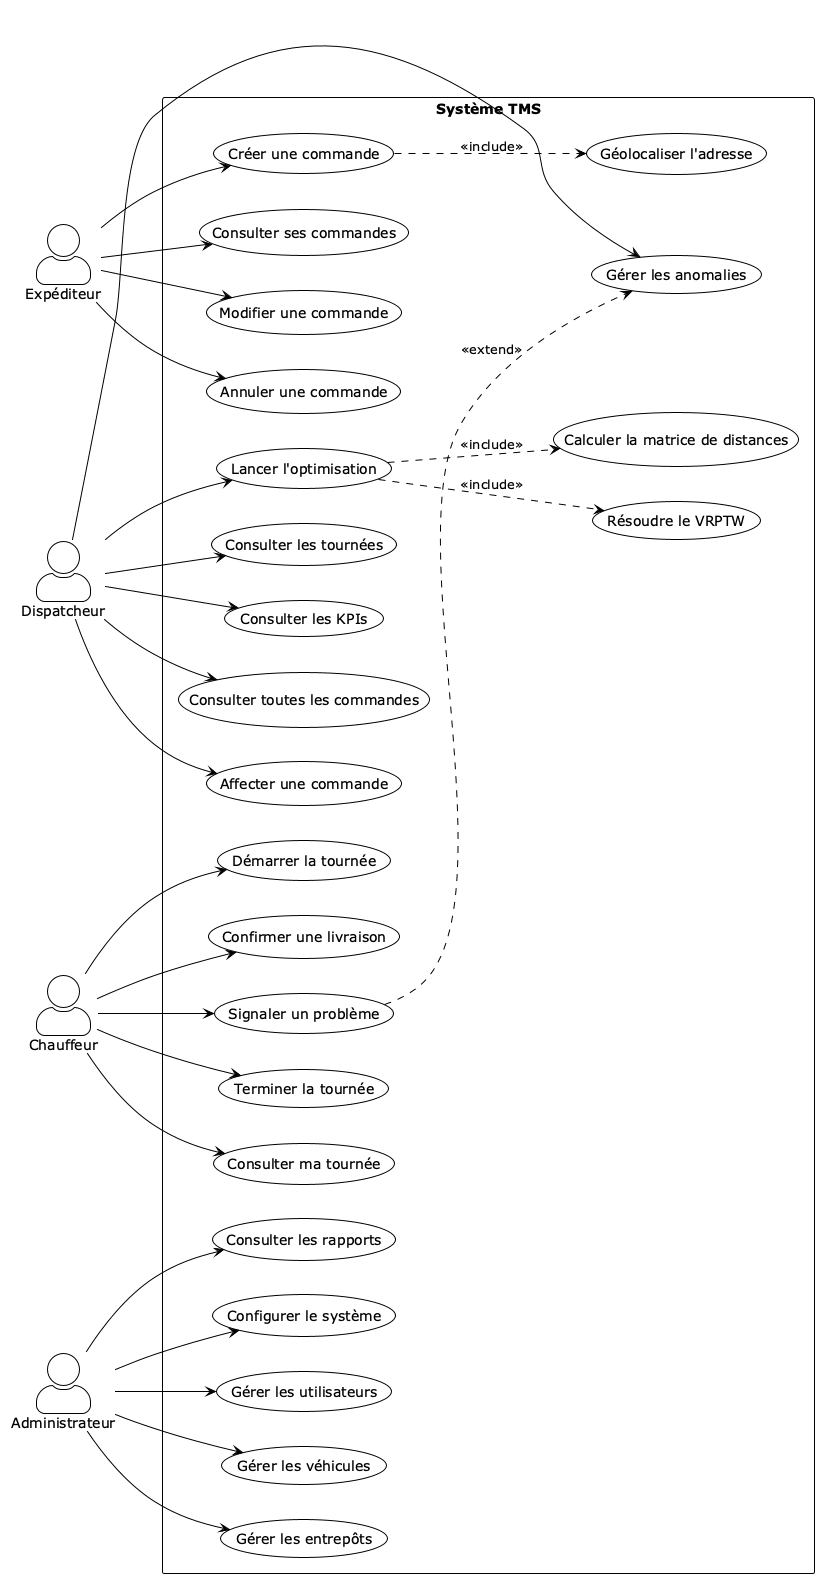
\includegraphics[height=0.82\textheight,keepaspectratio]{usecase.png}
   \caption{Diagramme de cas d'utilisation du TMS}
   \label{fig:use-case}
\end{figure}
\clearpage

\subsection{Diagramme de classes}

Le diagramme de classes (figure \ref{fig:class-diagram}) structure le modèle de données avec 8 entités : \textbf{Utilisateur} (rôles RBAC), \textbf{Warehouse} (dépôts multi-sites), \textbf{Vehicule} (capacités poids/volume + types), \textbf{Commande} (fenêtres de temps), \textbf{Tournee} (itinéraires), \textbf{StopTournee} (arrêts), \textbf{Anomalie} (incidents), et \textbf{TacheOptimisation} (traçabilité).

Les capacités doubles (poids ET volume) imposent deux contraintes simultanées dans le VRPTW. Le type de véhicule filtre les commandes compatibles (REFRIGERE/CONGELATEUR). Les clés étrangères préservent l'historique (pas de suppression en cascade).
 \begin{figure}[H]
   \centering
   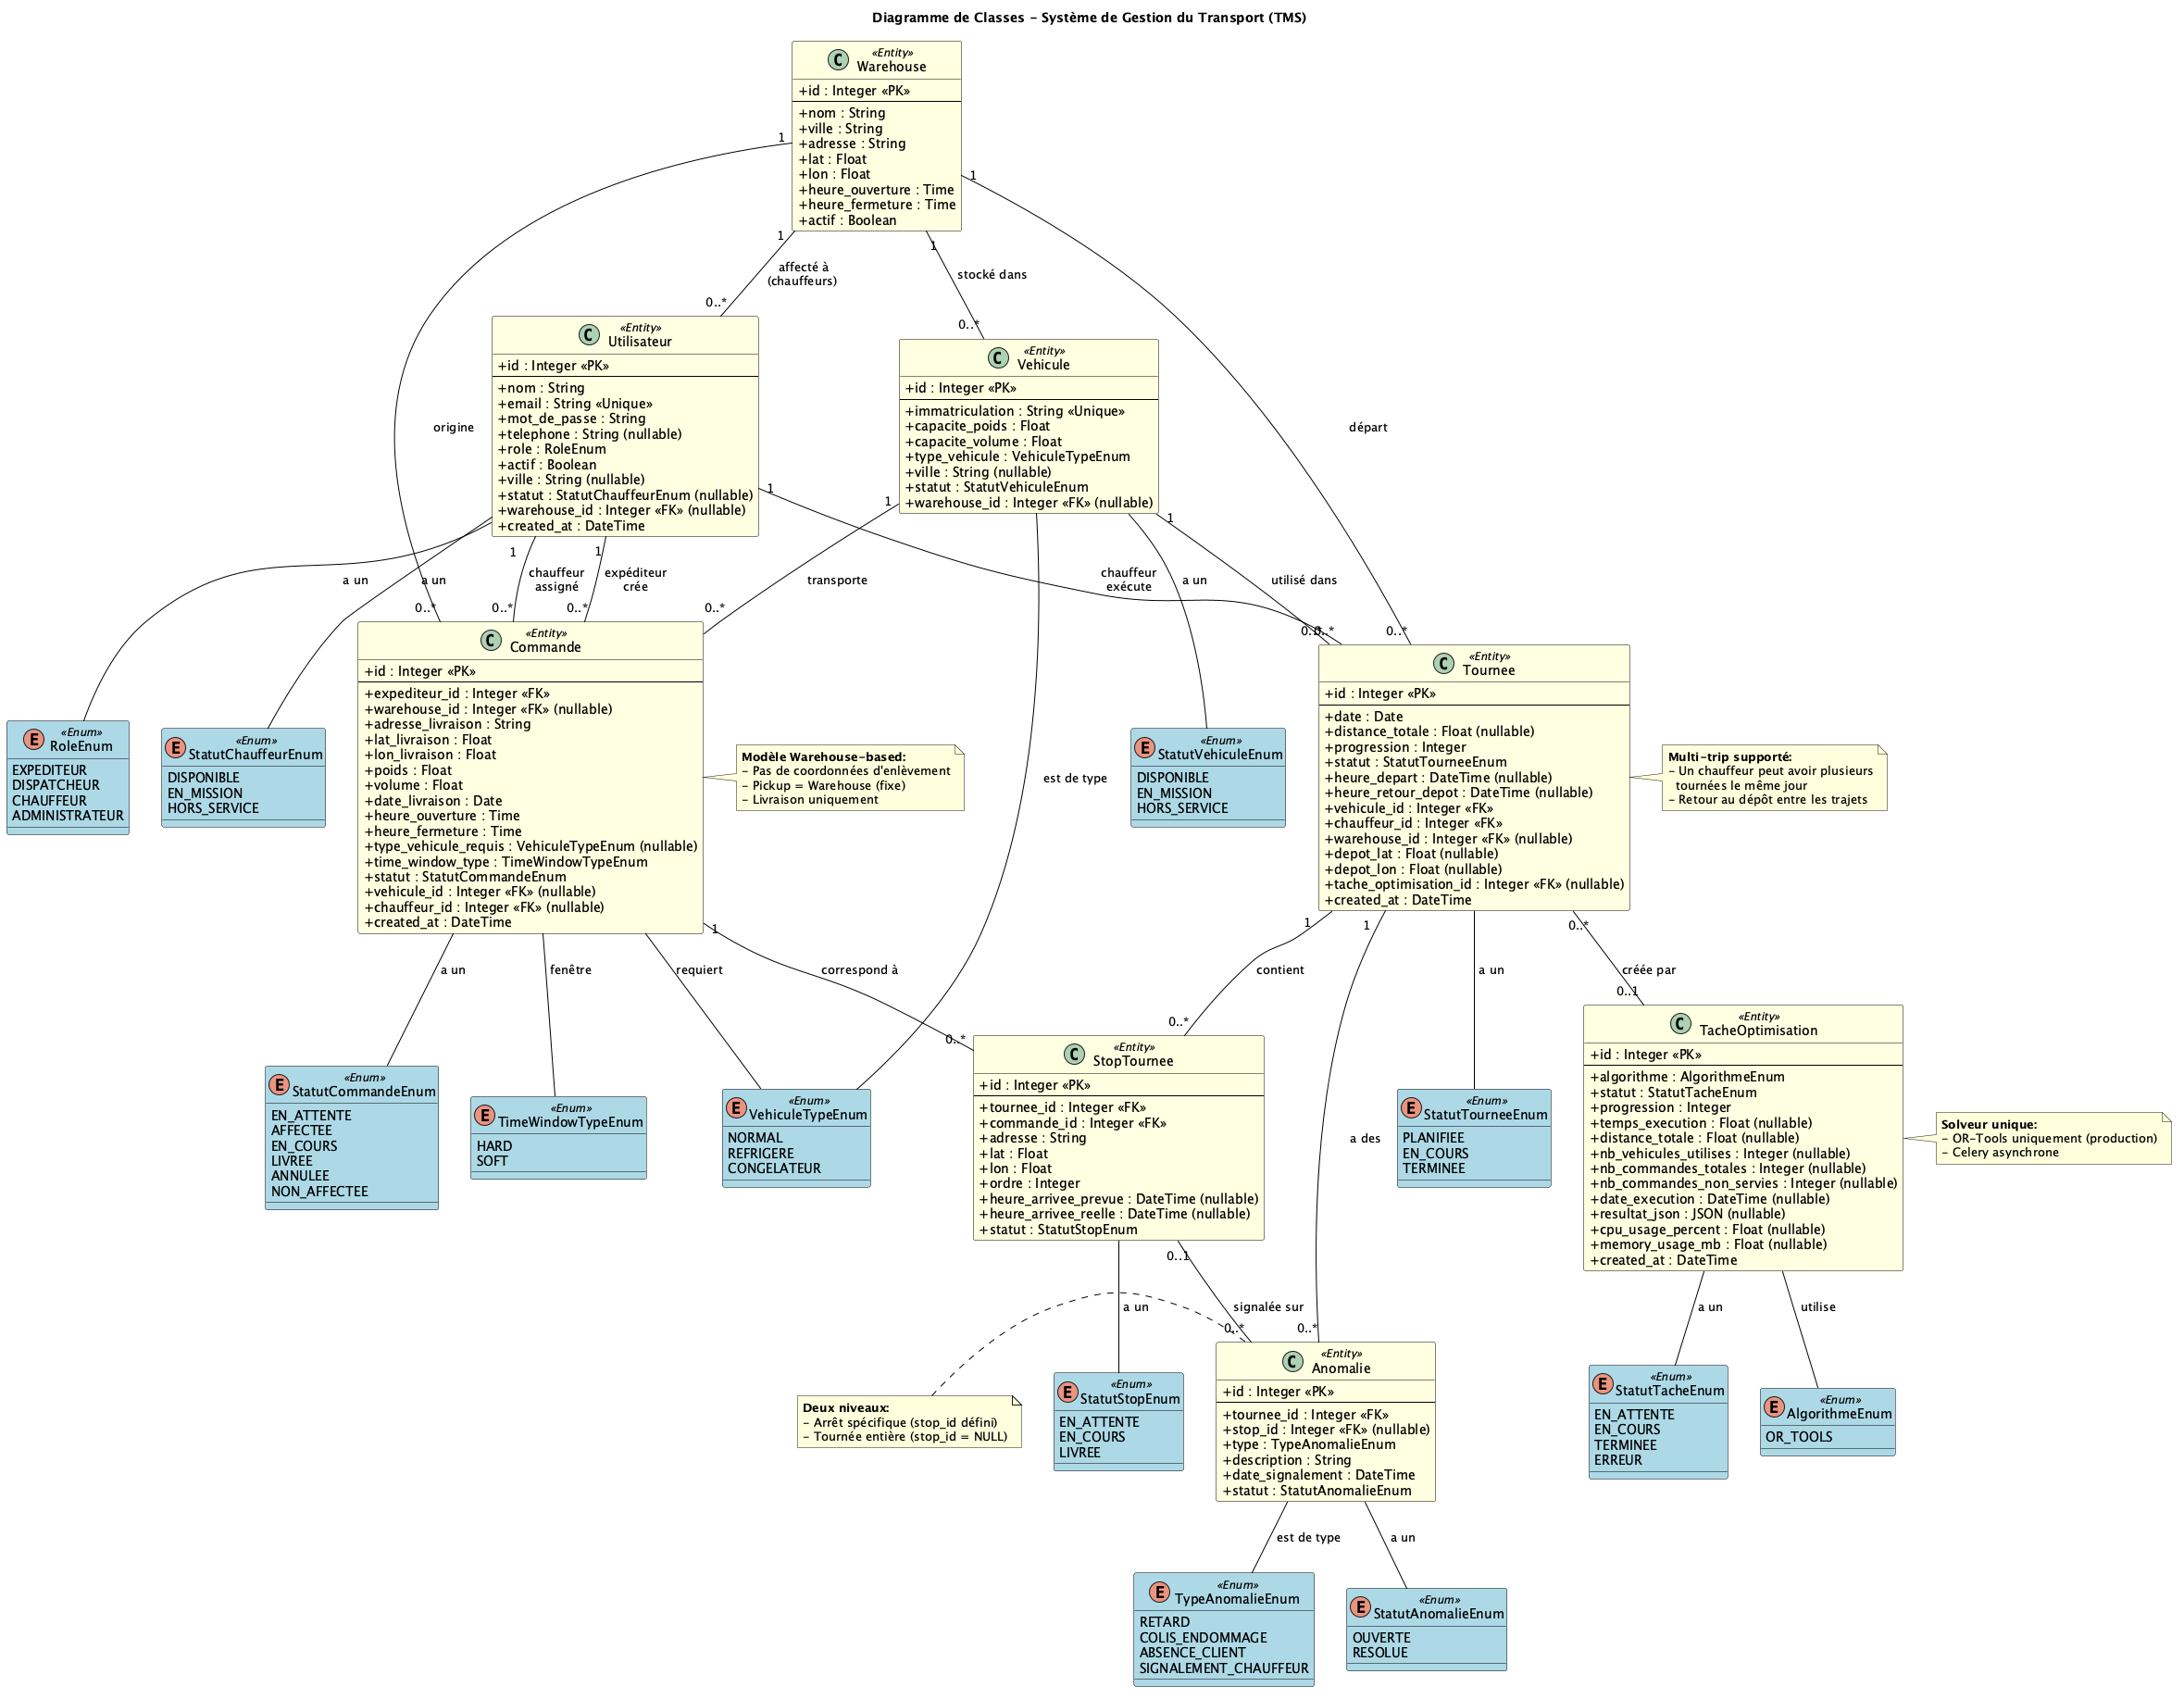
\includegraphics[width=\textwidth]{class_diagram.png}
   \caption{Diagramme de classes du TMS}
   \label{fig:class-diagram}
 \end{figure}

\subsection{Diagrammes de séquence}

Les diagrammes de séquence (figures \ref{fig:seq-create-order}, \ref{fig:seq-optimisation}, \ref{fig:seq-confirm-delivery}) présentent trois scénarios principaux du système.

\paragraph{Scénario 1 : Création d'une commande.}
Le géocodage est effectué côté frontend avant la soumission. L'expéditeur saisit une adresse, le frontend interroge d'abord Google Geocoding API, puis Nominatim (OpenStreetMap) en fallback si Google échoue. Les coordonnées (lat, lon) sont stockées dans le formulaire et affichées à l'utilisateur. \textbf{Point clé :} Si les deux services échouent, la validation côté client bloque la soumission du formulaire. Le backend reçoit une requête POST avec lat/lon déjà renseignés, valide la date de livraison (>= demain), puis enregistre la commande.

\paragraph{Scénario 2 : Lancement d'une optimisation (flux asynchrone).}
Le flux implique le Dispatcheur, l'API Backend, Redis (broker), un Worker Celery, le solveur OR-Tools, le service de routage (OSRM pour le calcul des matrices de distances/temps), et la base de données.

Le workflow est asynchrone : la requête HTTP retourne immédiatement (< 1s) avec un \texttt{tache\_id}, tandis que le calcul (30s-4.5min selon taille) s'exécute en arrière-plan. L'API et le Worker communiquent via Redis. Le Frontend interroge \texttt{GET /api/v1/optimisation/\{id\}/statut} toutes les 3 secondes pour suivre la progression. La matrice de distances complète est obtenue via requête unique à OSRM.

\paragraph{Scénario 3 : Confirmation de livraison.}
Le flux implique le Chauffeur, l'API Backend, et la base de données. \textbf{Point clé :} L'attribut \texttt{heure\_arrivee\_reelle} permet d'analyser a posteriori les écarts entre prévisions et réalité terrain (KPI : taux de respect des fenêtres).
 \begin{figure}[H]
   \centering
   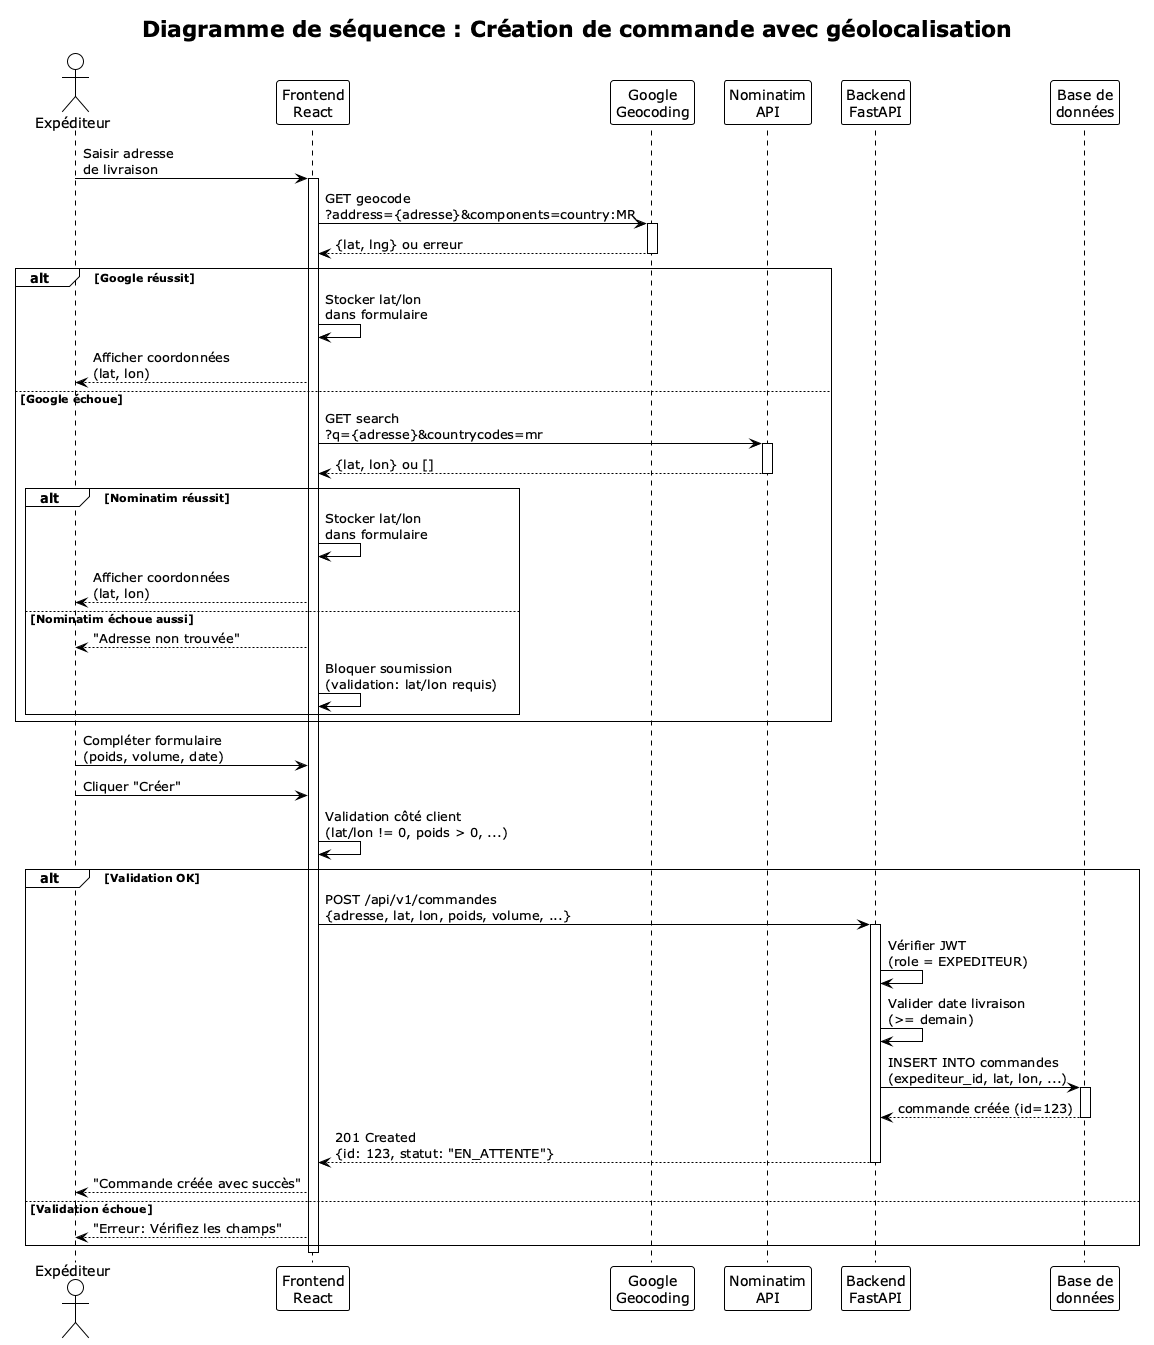
\includegraphics[width=0.9\textwidth]{sequence_create_order.png}
   \caption{Diagramme de séquence : Création d'une commande}
   \label{fig:seq-create-order}
 \end{figure}
 \begin{figure}[H]
   \centering
   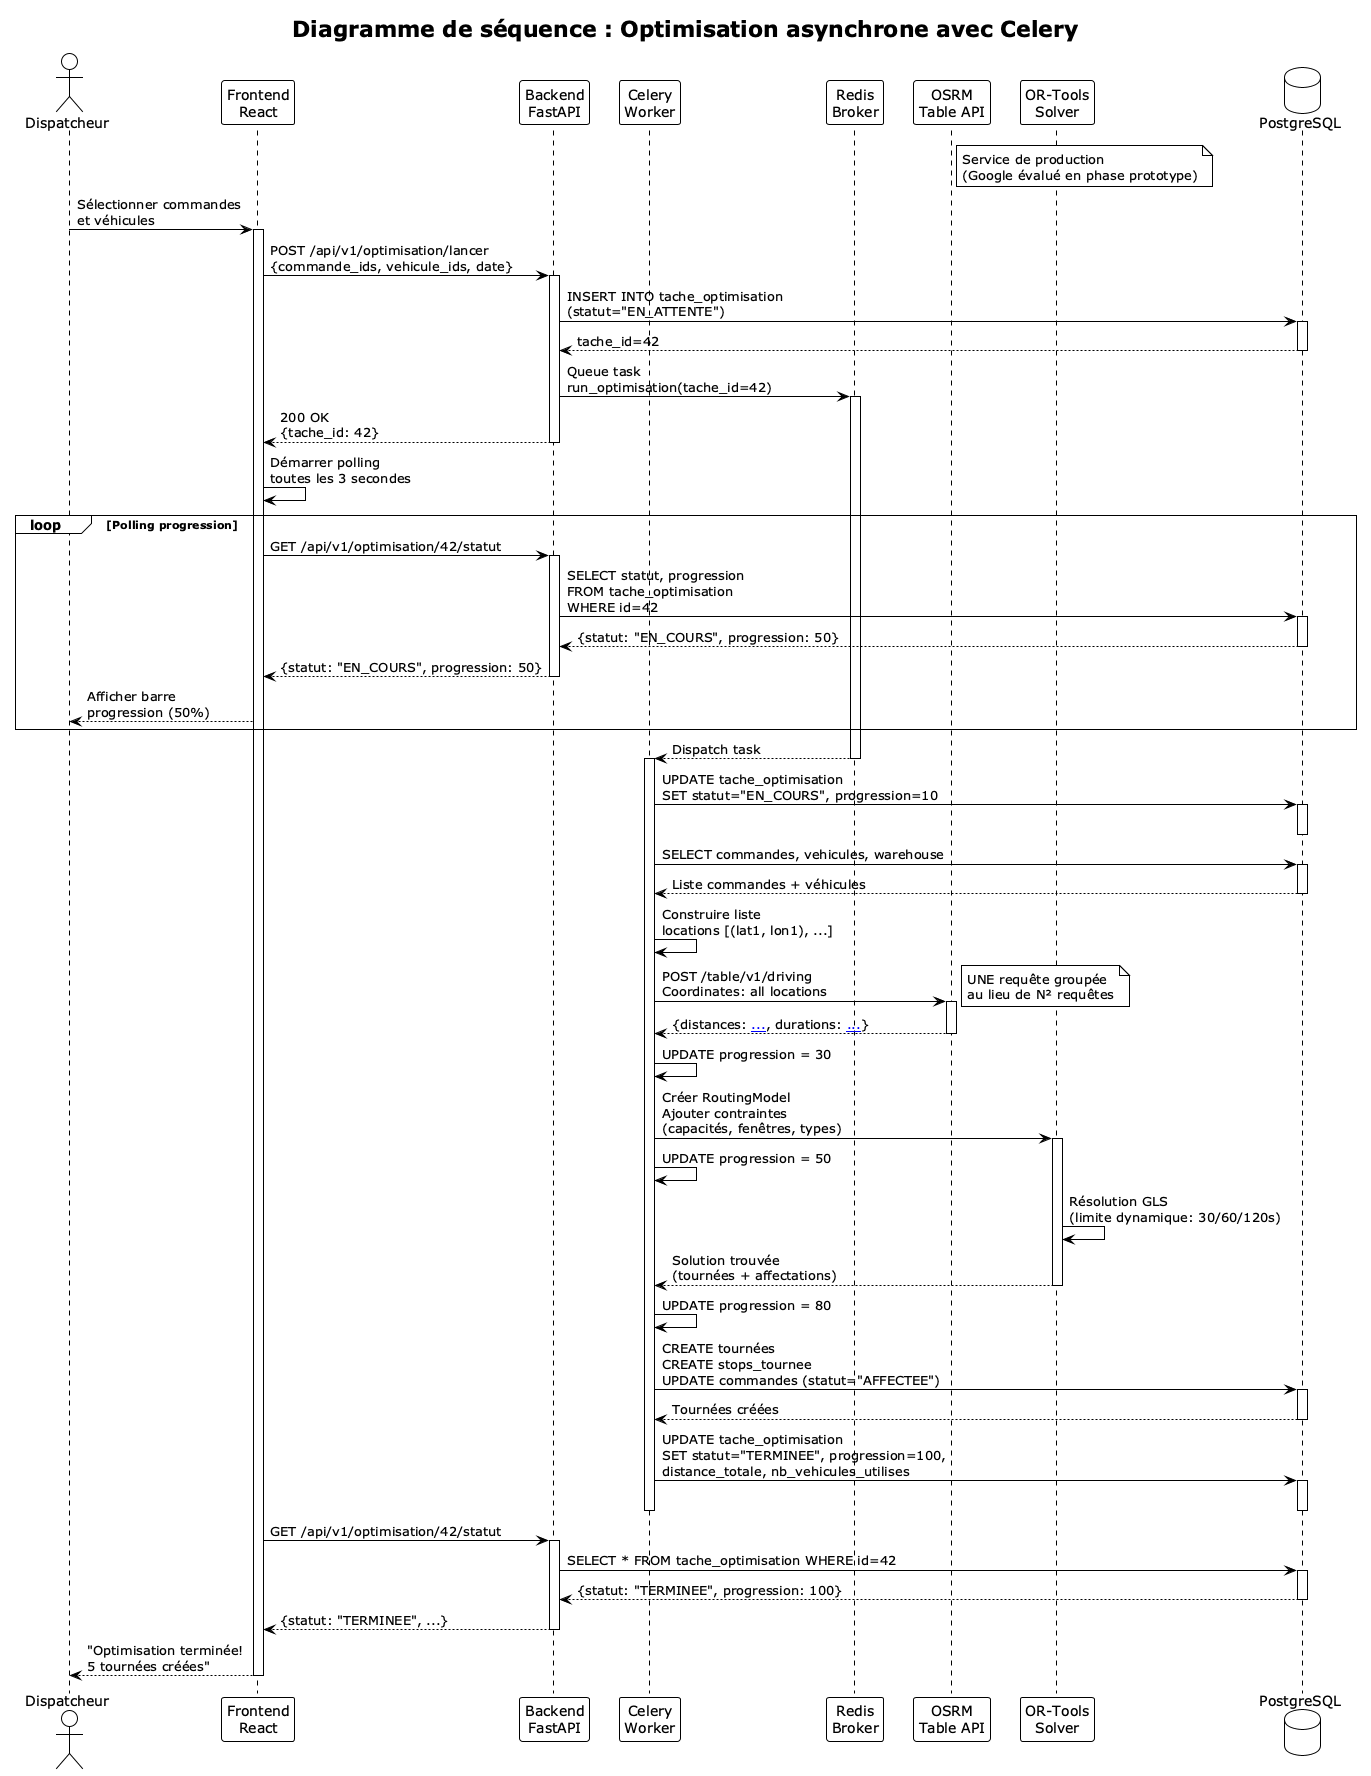
\includegraphics[width=\textwidth]{sequence_optimization.png}
   \caption{Diagramme de séquence : Lancement d'optimisation}
   \label{fig:seq-optimisation}
 \end{figure}
 \begin{figure}[H]
   \centering
   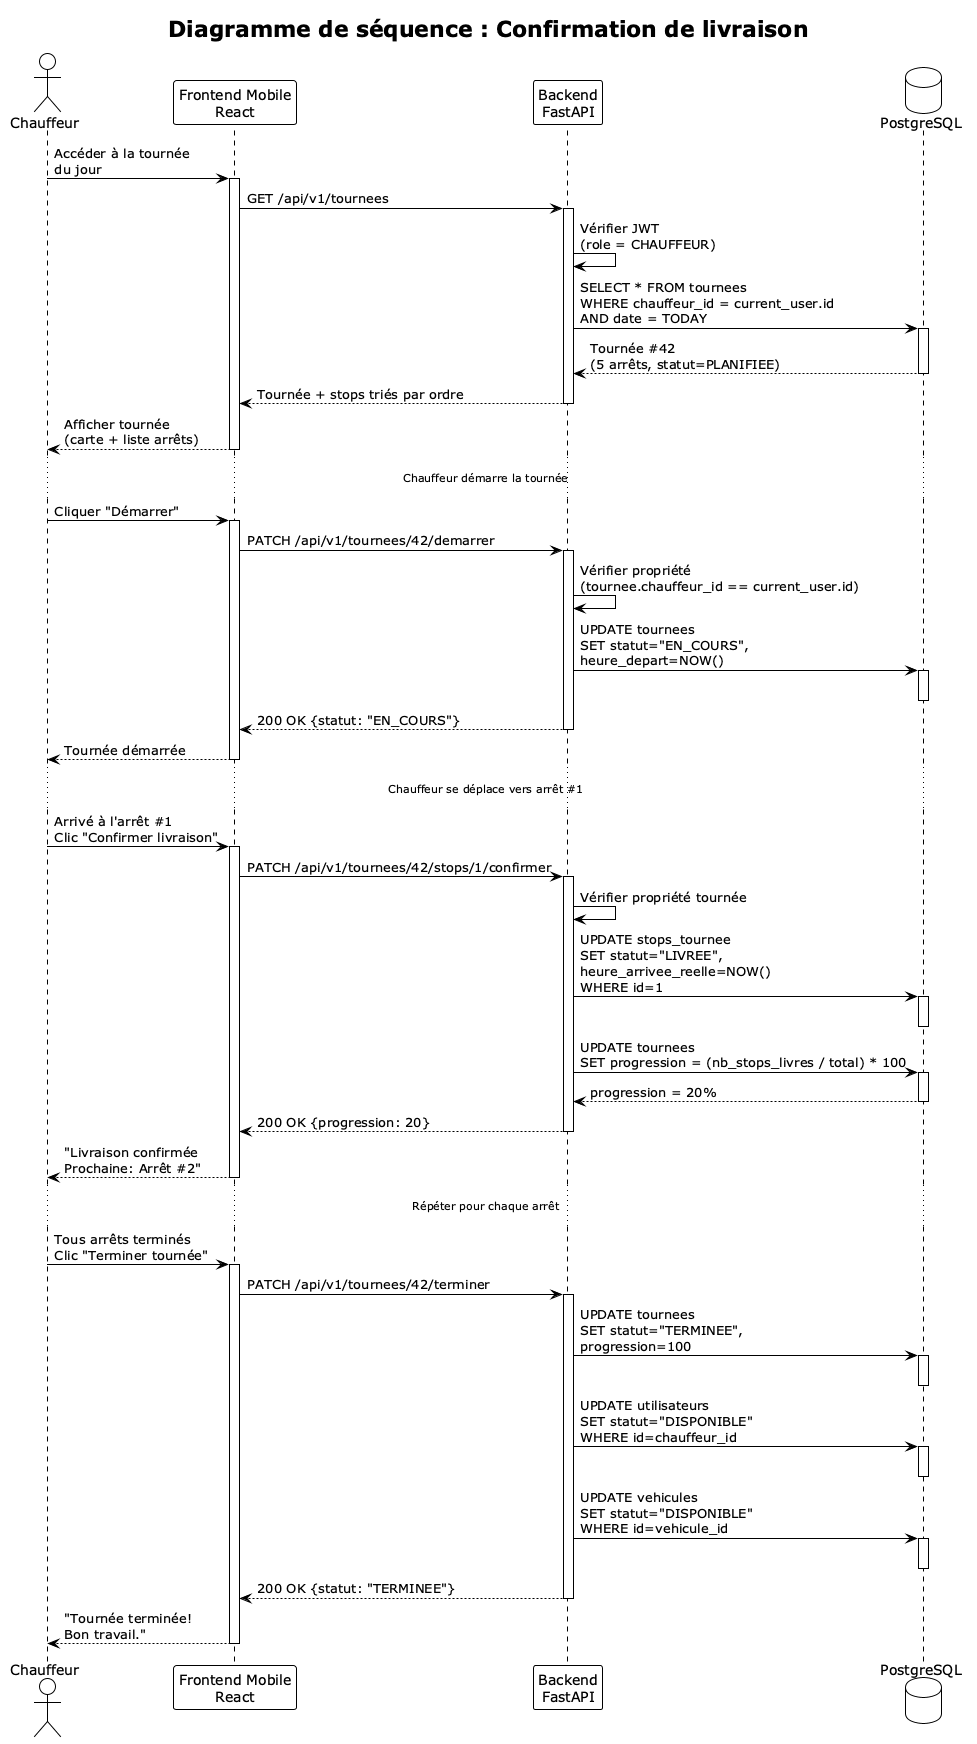
\includegraphics[width=0.8\textwidth]{sequence_confirm_delivery.png}
   \caption{Diagramme de séquence : Confirmation de livraison}
   \label{fig:seq-confirm-delivery}
\end{figure}

\section{Conception Mathématique : Le Modèle VRPTW}

Cette section formalise le problème d'optimisation des tournées comme un programme linéaire en nombres entiers (MILP — Mixed Integer Linear Program). Le modèle VRPTW (Vehicle Routing Problem with Time Windows) que nous présentons intègre plusieurs extensions pour refléter les contraintes opérationnelles identifiées au chapitre 1 : capacités multiples (poids et volume), types de véhicules hétérogènes, fenêtres de temps souples et dures, et support multi-trajets (un véhicule peut effectuer plusieurs tournées dans la journée en revenant se recharger au dépôt).

\subsection{Vue d'ensemble du modèle}

Le modèle présenté ci-après est un \emph{Problème de Tournées de Véhicules Multi-Trajets avec Fenêtres de Temps et Capacités Hétérogènes} (MT-VRPTW), une extension du problème de tournées de véhicules classique \cite{dantzig1959,toth2014}. Nous présentons les données, les variables de décision, l'objectif et les contraintes du modèle, puis une description du flux de résolution, incluant la décomposition multi-trajets avec temps de rechargement, la compatibilité de type de véhicule (affectation des commandes sensibles à la température aux véhicules adaptés) et un mode optionnel de fenêtres de temps souples. Le modèle est résolu par une métaheuristique (Recherche Locale Guidée \cite{voudouris1999,voudouris1997} appliquée à une solution initiale construite par l'heuristique du plus proche arc), motivée par la NP-difficulté du problème sous-jacent \cite{lenstra1981,garey1979}.

% =====================================================================
\subsubsection{Énoncé du Problème}
% =====================================================================

Un dépôt unique doit livrer un ensemble de commandes clients dans une
journée de travail, à l'aide d'une flotte limitée et contrainte en
capacité. Chaque commande possède une localisation géographique, une
demande en poids et en volume, et une fenêtre de temps durant laquelle elle
peut être servie. Chaque véhicule a une capacité en poids et une capacité
en volume, et doit commencer et terminer chaque trajet au dépôt dans les
heures d'ouverture de celui-ci. Un véhicule peut effectuer plus d'un trajet
par jour : après être revenu au dépôt, il peut être rechargé (ce qui prend
un temps de chargement fixe) puis renvoyé en tournée.

L'objectif est de servir le plus de commandes possible tout en minimisant,
par priorité lexicographique, d'abord le nombre de véhicules utilisés puis
la distance totale parcourue. Les commandes qui ne peuvent pas être servies
de façon réalisable peuvent rester non servies, moyennant une pénalité.
Cette structure relève de la famille des problèmes de tournées de véhicules
avec fenêtres de temps (VRPTW) \cite{solomon1987,toth2014}.

% =====================================================================
\subsubsection{Notations et Données}
% =====================================================================

\subsection{Ensembles et indices}

\begin{itemize}[leftmargin=2.2em]
  \item $C = \{1, 2, \dots, n\}$ --- l'ensemble des commandes clients.
  \item Le nœud $0$ --- le dépôt. L'ensemble des nœuds est $N = \{0\} \cup C$.
  \item $A = \{(i,j) : i,j \in N,\ i \neq j\}$ --- l'ensemble des arcs
        orientés.
  \item $K = \{1, 2, \dots, m\}$ --- l'ensemble des véhicules disponibles
        (après limitation de la flotte au nombre de chauffeurs disponibles ;
        voir la Section~\ref{sec:flux}).
  \item $T$ --- l'ensemble des types de véhicule (régimes de température),
        p.\,ex. $\{\text{normal},\ \text{réfrigéré},\ \text{congélateur}\}$.
\end{itemize}

\subsection{Paramètres}

\begin{itemize}[leftmargin=2.2em]
  \item $d_{ij} \in \R_+$ --- distance routière (km) du nœud $i$ au
        nœud $j$, obtenue du service de routage (OSRM en production).
  \item $t_{ij} \in \Zp$ --- temps de trajet routier (secondes) du nœud $i$
        au nœud $j$.
  \item $s_i \in \Zp$ --- temps de service (manutention) au nœud $i$. À
        chaque client $s_i = \sigma$ (une constante, p.\,ex. $\sigma = 600$
        s $= 10$ min). Au dépôt $s_0 = \delta$, le \emph{temps de service au
        dépôt} (chargement/rechargement), une constante configurable ; voir
        la Remarque~\ref{rem:depot}.
  \item $q_i^{\mathrm w}, q_i^{\mathrm v} \in \R_+$ --- demande en
        poids et en volume de la commande $i$ ($q_0^{\mathrm w} =
        q_0^{\mathrm v} = 0$).
  \item $Q_k^{\mathrm w}, Q_k^{\mathrm v} \in \R_+$ --- capacité en
        poids et en volume du véhicule $k$.
  \item $\tau_k \in T$ --- type (régime de température) du véhicule $k$.
  \item $\hat{\tau}_i \in T \cup \{\varnothing\}$ --- type requis par la
        commande $i$. La valeur $\varnothing$ (aucune exigence explicite)
        est traitée comme « normal » ; voir la Remarque~\ref{rem:type}.
  \item $[e_i, \ell_i]$ --- la fenêtre de temps de la commande $i$, en
        secondes depuis minuit, où $e_i$ est l'heure de début de service au
        plus tôt et $\ell_i$ au plus tard.
  \item $[E, L]$ --- la fenêtre d'ouverture du dépôt ($E$ = ouverture, $L$ =
        fermeture), en secondes depuis minuit.
  \item $\delta \in \Zp$ --- le temps de service au dépôt (chargement en
        début de trajet ; de façon équivalente, le temps de
        rechargement/rotation entre deux trajets consécutifs d'un même
        véhicule, ces deux opérations étant la même opération physique au
        quai). Configurable ; valeur par défaut $\delta = 3600$~s.
  \item $\alpha \in \R_+$ --- coût par véhicule utilisé.
  \item $\beta \in \R_+$ --- coût par kilomètre parcouru.
  \item $P \in \R_+$ --- pénalité pour une commande laissée non servie.
\end{itemize}

\begin{remarque}[Prétraitement des fenêtres de temps]
Une fenêtre client ouvrant avant le dépôt, $e_i < E$, est ramenée à
$e_i \leftarrow E$, puisqu'aucun véhicule ne peut partir avant l'ouverture
du dépôt. Si, après ce recalage, $\ell_i \leq e_i$, la fenêtre est élargie à
celle du dépôt afin d'éviter un intervalle vide (infaisable) ; une telle
commande ne sera servie que si la temporisation de la tournée le permet, ou
sera sinon laissée non servie.
\end{remarque}

\begin{remarque}[Temps de service au dépôt et plancher de départ unifié]
\label{rem:depot}
Charger un véhicule en début de trajet et le recharger entre deux trajets
sont la même opération physique au quai ; le modèle utilise donc un unique
paramètre configurable $\delta$ pour les deux. Un véhicule ne peut pas
partir avant d'avoir été chargé, et le chargement ne peut commencer avant
que le véhicule ne soit présent au dépôt et que le dépôt ne soit ouvert.
Cela donne une règle unique régissant l'heure de départ $a_0^{(k)}$ de
\emph{chaque} trajet du véhicule $k$ :
%
\begin{equation}
  a_0^{(k)} \;\geq\; b_k + \delta,
  \label{eq:plancher}
\end{equation}
%
où $b_k$ est l'instant à partir duquel le chargement de ce trajet peut
commencer :
%
\[
  b_k =
  \begin{cases}
    E, & \text{premier trajet (chargement possible dès l'ouverture),}\\[2pt]
    \text{heure de retour de } k, & \text{trajets suivants (chargement dès le retour de $k$).}
  \end{cases}
\]
%
Ainsi le \textbf{premier trajet} ne peut partir avant $E + \delta$ (le dépôt
doit être ouvert assez longtemps pour charger), et un \textbf{second trajet}
ne peut partir avant son heure de disponibilité
$r_k = (\text{heure de retour de } k) + \delta$, ce qui est exactement
\eqref{eq:plancher} avec $b_k$ fixé à l'heure de retour.

\paragraph{Comptabilisé une seule fois.}
Comme le flux multi-trajets (Section~\ref{sec:flux}) résout chaque trajet
comme une instance de modèle distincte, $\delta$ est réalisé comme le
\textbf{plancher de départ}~\eqref{eq:plancher} de chaque trajet, et le
temps de service au dépôt \emph{à l'intérieur} d'une tournée est pris égal à
$0$ ($s_0 = 0$ dans la propagation), de sorte que le chargement est
comptabilisé par le plancher et jamais une seconde fois dans la tournée. En
pratique, le plancher du premier trajet est réalisé en décalant l'heure
d'ouverture vue par le solveur de $E$ à $E + \delta$.

\paragraph{Chargement au plus tard (présentation uniquement).}
La contrainte~\eqref{eq:plancher} ne fixe que le départ \emph{au plus tôt} ;
elle n'oblige pas le véhicule à être chargé dès $b_k$ puis à attendre. Si le
départ choisi est $d \geq b_k + \delta$, le chargement peut être rapporté
comme occupant l'intervalle $[\,d - \delta,\ d\,]$ --- c'est-à-dire un
chargement au plus tard, terminé juste avant le départ. Il s'agit d'un choix
de présentation à l'étape d'extraction de la solution ; il ne change pas
l'ensemble réalisable.
\end{remarque}


\subsubsection{Variables de Décision}


\begin{itemize}[leftmargin=2.2em]
  \item $x_{ijk} \in \{0,1\}$ --- vaut $1$ si le véhicule $k$ se déplace
        directement du nœud $i$ au nœud $j$, et $0$ sinon.
  \item $y_k \in \{0,1\}$ --- vaut $1$ si le véhicule $k$ est utilisé
        (effectue au moins un trajet), et $0$ sinon.
  \item $z_i \in \{0,1\}$ --- vaut $1$ si la commande $i$ est \emph{servie},
        et $0$ si elle est laissée non servie.
  \item $a_i \in \Zp$ --- l'instant où le service \emph{commence} au nœud
        $i$ (l'heure d'arrivée, éventuellement après attente).
  \item $w_i^{\mathrm w}, w_i^{\mathrm v} \in \R_{\geq 0}$ --- la charge
        cumulée (poids, volume) à l'arrivée au nœud $i$.
\end{itemize}

% =====================================================================
\subsubsection{Fonction Objectif}
% =====================================================================

L'optimisation minimise un coût pondéré unique combinant la taille de la
flotte, la distance et les pénalités de commandes non servies :
%
\begin{equation}
  \min \;\;
    \underbrace{\alpha \sum_{k \in K} y_k}_{\text{coût de flotte}}
    \;+\;
    \underbrace{\beta \sum_{k \in K} \sum_{(i,j) \in A} d_{ij}\, x_{ijk}}_{\text{coût de distance}}
    \;+\;
    \underbrace{P \sum_{i \in C} (1 - z_i)}_{\text{pénalité de non-service}} .
  \label{eq:objectif}
\end{equation}
%
Les deux premiers termes reproduisent l'objectif multicritère classique du
VRP $\min\bigl(\alpha \sum_k y_k + \beta \sum_{ijk} d_{ij} x_{ijk}\bigr)$
\cite{toth2014}. Le troisième terme, actif uniquement lorsque le service
partiel est autorisé, valorise la décision d'abandonner une commande ;
ce mécanisme correspond aux disjonctions du solveur \cite{ortools}.

\paragraph{Calibrage des coûts.}
Les magnitudes relatives de $\alpha$, $\beta$ et $P$ encodent l'ordre de
priorité voulu et doivent satisfaire deux conditions :
%
\begin{align}
  \alpha &\gg \beta \cdot (\text{diamètre du réseau en km}),
  \label{eq:cal1}\\
  P &> \alpha .
  \label{eq:cal2}
\end{align}
%
La condition~\eqref{eq:cal1} fait que l'activation d'un véhicule
supplémentaire domine toute économie de distance, de sorte que le modèle
minimise d'abord le nombre de véhicules puis la distance (comportement
lexicographique par pondérations scalaires). La condition~\eqref{eq:cal2}
assure que la pénalité d'abandon dépasse le coût fixe d'activation d'un
véhicule ; sans elle, le solveur pourrait abandonner tout un camion de
commandes plutôt que d'activer ce véhicule, car le coût fixe économisé
$\alpha$ dépasserait les pénalités accumulées. Dans l'implémentation, on
utilise $P = \alpha + 1000\,\beta$ (en unités de coût mises à l'échelle).

\paragraph{Calibrage strict (tenant compte de la distance).}
La condition~\eqref{eq:cal2} ne tient pas compte de la distance parcourue.
À elle seule, elle n'oblige pas à servir une commande unique très éloignée :
si l'atteindre
coûte $\alpha + \beta\,d_{0i} > P$, le solveur l'abandonnera rationnellement,
traitant $P$ comme le \emph{seuil de valeur} en deçà duquel une commande ne
vaut pas un trajet dédié. Pour servir toute commande \emph{réalisable} quelle
que soit la distance, on renforce \eqref{eq:cal2} en
%
\begin{equation}
  P \;>\; \alpha + \beta D,
  \label{eq:cal2strict}
\end{equation}
%
où $D$ borne la plus longue tournée possible d'un véhicule. La valeur par
défaut $P = \alpha + 1000\beta$ réalise \eqref{eq:cal2strict} sous
l'hypothèse qu'aucune tournée ne dépasse $\approx 1000$~km, ce qui convient à
une exploitation à l'échelle urbaine ou régionale.

\begin{remarque}[Mise à l'échelle entière]
Le solveur exige des coûts d'arc entiers \cite{ortools}. Tous les coûts
réels sont convertis en entiers via un unique facteur d'échelle $S$ (unités
de coût par km) : une distance $d_{ij}$ devient $\lfloor d_{ij}\, S \rceil$,
le coût fixe de véhicule devient $\lfloor \alpha\, S \rceil$, et la pénalité
devient $\lfloor P\, S \rceil$. Utiliser un \emph{unique} facteur pour
\emph{tous} les termes de coût est essentiel ; mélanger les échelles fausse
silencieusement les arbitrages de \eqref{eq:objectif}.
\end{remarque}

% =====================================================================
\subsubsection{Contraintes}
% =====================================================================

La formulation suit les formulations classiques en flot du VRP
\cite{toth2014,solomon1987}.

\subsection{Contraintes de routage et de degré}

Chaque client servi est entré et quitté exactement une fois ; un client non
servi n'est pas visité :
%
\begin{align}
  \sum_{k \in K} \sum_{j \in N,\, j \neq i} x_{ijk} &= z_i,
    && \forall i \in C, \label{eq:sortie}\\
  \sum_{k \in K} \sum_{j \in N,\, j \neq i} x_{jik} &= z_i,
    && \forall i \in C. \label{eq:entree}
\end{align}
%
La conservation du flot assure que tout ce qui entre dans un nœud en ressort
sur le même véhicule :
%
\begin{equation}
  \sum_{j \in N,\, j \neq h} x_{jhk}
  \;=\;
  \sum_{j \in N,\, j \neq h} x_{hjk},
  \qquad \forall h \in C,\ \forall k \in K.
  \label{eq:flot}
\end{equation}

\subsection{Utilisation des véhicules et degré au dépôt}

Un véhicule utilisé quitte le dépôt et y revient ; un véhicule inutilisé
reste à l'arrêt :
%
\begin{align}
  \sum_{j \in C} x_{0jk} &= y_k, && \forall k \in K, \label{eq:depotsortie}\\
  \sum_{i \in C} x_{i0k} &= y_k, && \forall k \in K. \label{eq:depotentree}
\end{align}
%
(Dans le flux multi-trajets de la Section~\ref{sec:flux}, chaque trajet est
un problème de routage distinct ; \eqref{eq:depotsortie}--\eqref{eq:depotentree}
s'appliquent donc par trajet.)

\subsection{Contraintes de capacité}

La charge cumulée est propagée le long de chaque arc et bornée par la
capacité du véhicule qui le parcourt. Pour tout $(i,j) \in A$ et $k \in K$ :
%
\begin{align}
  x_{ijk} = 1 \;\Longrightarrow\;
    w_j^{\mathrm w} &= w_i^{\mathrm w} + q_j^{\mathrm w},
    & w_i^{\mathrm w} &\leq Q_k^{\mathrm w}, \label{eq:capp}\\
  x_{ijk} = 1 \;\Longrightarrow\;
    w_j^{\mathrm v} &= w_i^{\mathrm v} + q_j^{\mathrm v},
    & w_i^{\mathrm v} &\leq Q_k^{\mathrm v}. \label{eq:capv}
\end{align}
%
Le poids et le volume sont suivis comme deux dimensions de capacité
indépendantes ; une affectation n'est réalisable que si elle respecte les
\emph{deux}.

\subsection{Propagation temporelle et journée de travail}

Les heures de début de service sont propagées le long des arcs, en ajoutant
le temps de trajet et de service. Pour tout $(i,j) \in A$, $k \in K$ :
%
\begin{equation}
  x_{ijk} = 1 \;\Longrightarrow\;
  a_j \;\geq\; a_i + s_i + t_{ij}.
  \label{eq:proptemps}
\end{equation}
%
L'inégalité (plutôt que l'égalité) autorise l'\emph{attente} : un véhicule
arrivant avant $e_j$ peut attendre l'ouverture de la fenêtre. Toute
l'activité est confinée à la journée de travail du dépôt :
%
\begin{equation}
  E \;\leq\; a_i \;\leq\; L, \qquad \forall i \in N.
  \label{eq:journee}
\end{equation}
%
L'heure de \emph{départ} du dépôt est bornée plus finement que le générique
$a_i \geq E$ : un véhicule ne peut partir avant d'être chargé, donc son
départ de premier trajet vérifie $a_0^{(k)} \geq E + \delta$, le plancher de
la Remarque~\ref{rem:depot}, équation~\eqref{eq:plancher}.

\begin{remarque}[Élimination implicite des sous-tours]
Les contraintes de flot \eqref{eq:sortie}--\eqref{eq:flot} n'interdisent pas,
à elles seules, les sous-tours déconnectés. C'est la propagation temporelle
\eqref{eq:proptemps} qui joue ce rôle : comme l'heure de service croît
strictement le long de chaque arc ($a_j \geq a_i + s_i + t_{ij}$ avec
$s_i + t_{ij} > 0$), aucun nœud ne peut se précéder lui-même dans le temps,
ce qui rend tout cycle fermé ne passant pas par le dépôt infaisable. La
variable temporelle $a_i$ joue donc le rôle des variables d'ordre de
Miller--Tucker--Zemlin \cite{miller1960} : elle élimine les sous-tours sans
qu'il soit nécessaire d'ajouter des contraintes dédiées.
\end{remarque}

\begin{remarque}[Horizon en temps absolu]
La variable $a_i$ est un temps \emph{absolu} d'horloge (secondes depuis
minuit), et non une durée écoulée. Par conséquent, la borne supérieure qui
plafonne la dimension temporelle doit être l'heure de \emph{fermeture} du
dépôt $L$, et non la durée de journée $L-E$. Cette distinction est cruciale
pour les trajets démarrant tard dans la journée (Section~\ref{sec:flux}) :
borner par $L-E$ tronquerait silencieusement toute tournée dont le temps
absolu dépasse $E + (L-E)$ calculé à partir d'un départ matinal, rendant les
départs tardifs faussement infaisables.
\end{remarque}

\subsection{Fenêtres de temps --- mode dur (par défaut)}

Dans la formulation par défaut, les fenêtres sont dures : le service ne peut
commencer ni avant $e_i$ ni après $\ell_i$ \cite{solomon1987}.
%
\begin{equation}
  z_i = 1 \;\Longrightarrow\; e_i \;\leq\; a_i \;\leq\; \ell_i,
  \qquad \forall i \in C.
  \label{eq:dur}
\end{equation}
%
Une commande dont la fenêtre ne peut être respectée est forcée à $z_i = 0$
(non servie) et encourt la pénalité $P$ dans \eqref{eq:objectif}.

\subsection{Fenêtres de temps --- mode souple (optionnel)}
\label{sec:souple}

Les fenêtres dures sont pessimistes pour la logistique réelle, où de
nombreuses fenêtres expriment une \emph{préférence} plutôt qu'une règle
stricte. Dans le mode souple optionnel, une commande peut être servie après
$\ell_i$ moyennant une pénalité de retard, jusqu'à une limite de grâce
$\ell_i + g$ ($g$ = période de grâce). L'heure au plus tôt $e_i$ reste dure
(un véhicule ne peut servir avant l'ouverture du client). On remplace la
borne supérieure de \eqref{eq:dur} par une borne souple pénalisée et on
augmente l'objectif. Soit le retard de la commande $i$ :
%
\begin{equation}
  \lambda_i \;=\; \max\bigl(0,\; a_i - \ell_i\bigr),
  \qquad 0 \leq \lambda_i \leq g .
  \label{eq:retard}
\end{equation}
%
Le service est permis sur $[e_i,\ \ell_i + g]$, et l'objectif gagne un terme
de retard :
%
\begin{equation}
  \min \quad (\text{Éq.}~\ref{eq:objectif})
    \;+\; \gamma \sum_{i \in C} \lambda_i \, z_i,
  \label{eq:objsouple}
\end{equation}
%
où $\gamma > 0$ est le coût de retard par unité de temps. Au-delà de
$\ell_i + g$, la commande ne peut qu'être laissée non servie (ou reportée à
un trajet ultérieur). Cette borne souple est réalisée dans le solveur par
une borne supérieure pénalisée sur la dimension temporelle \cite{ortools}.

\paragraph{Calibrage de la pénalité de retard.}
La pente de retard $\gamma$ est fixée en exigeant qu'un retard égal à
\emph{toute} la période de grâce $g$ coûte approximativement autant que
l'abandon de la commande :
%
\begin{equation}
  \gamma \cdot g \;\approx\; P
  \qquad\Longrightarrow\qquad
  \gamma \;=\; \frac{P}{g}.
  \label{eq:gamma}
\end{equation}
%
Cela produit l'ordre de préférence voulu
%
\[
  \text{à l'heure} \;\prec\; \text{légèrement en retard}
  \;\prec\; \text{très en retard} \;\prec\; \text{abandon}.
\]
%
Le choix entre borne dure \eqref{eq:dur} et borne souple
\eqref{eq:retard}--\eqref{eq:objsouple} est une propriété par commande ; une
même instance peut donc mélanger clients stricts et flexibles.

\subsection{Contrainte de type de véhicule (régime de température)}
\label{sec:type}

Chaque véhicule possède un \emph{unique} type $\tau_k \in T$ définissant le
régime de température de \emph{tout} son chargement sur une tournée (ambiant,
réfrigéré, surgelé). Comme toutes les commandes d'une même tournée partagent
le même compartiment à la même température, elles doivent toutes exiger ce
même régime. La contrainte est une égalité de type : la commande $i$ ne peut
être servie que par un véhicule $k$ tel que $\tau_k = \hat{\tau}_i$ :
%
\begin{equation}
  x_{ijk} = 1 \;\Longrightarrow\; \tau_k = \hat{\tau}_i,
  \qquad \forall i \in C,\ \forall j \in N,\ \forall k \in K.
  \label{eq:type}
\end{equation}
%
En pratique, pour chaque commande, on restreint l'ensemble des véhicules
admissibles à son nœud à ceux du type requis \cite{ortools}.

\begin{remarque}[Type unique plutôt que compétences multiples]
\label{rem:type}
Le modèle attribue à chaque véhicule un \emph{seul} type, et non un ensemble
de compétences. Ce choix reflète le fait que la température est une propriété
du \emph{compartiment entier} : on ne peut pas mélanger des marchandises
ambiantes et réfrigérées dans le même camion. Une commande sans type
explicite ($\hat{\tau}_i = \varnothing$) est traitée comme « normal »
(ambiant) ; elle ne peut donc pas voyager dans un camion réfrigéré ou
congélateur qui roule en froid pour ses autres commandes. Ce modèle
\emph{strict} évite qu'une marchandise ambiante soit refroidie, ou qu'une
marchandise froide soit réchauffée. Son coût est une réduction de la
flexibilité : si la flotte ne comporte aucun véhicule du type requis, la
commande est laissée non servie plutôt que mal affectée.
\end{remarque}

\subsection{Domaines des variables}

\begin{equation}
  x_{ijk}, y_k, z_i \in \{0,1\}; \qquad
  a_i \in \Zp; \qquad
  w_i^{\mathrm w}, w_i^{\mathrm v} \in \R_{\geq 0}.
\end{equation}

\begin{remarque}[Véhicule inutilisé et commandes non servies peuvent coexister, mais seulement sous infaisabilité]
\label{rem:inutilise}
Une solution peut présenter un véhicule inutilisé ($y_k = 0$) en même temps
que des commandes non servies ($z_i = 0$). Sous le calibrage strict tenant
compte de la distance (condition~\eqref{eq:cal2strict}), ce n'est \emph{pas}
un signe de paresse mais d'infaisabilité réelle. Deux cas se présentent :
\begin{enumerate}[leftmargin=2.2em]
  \item \textbf{Commandes servables, véhicule inutilisé --- exclu.} Si un
        véhicule inutilisé pouvait servir une commande non servie (capacité,
        fenêtre et type le permettant), alors l'activer coûte $\alpha +
        \beta d$ tandis que l'abandonner coûte $P$ ; sous
        \eqref{eq:cal2strict}, servir reste moins coûteux que l'abandon. Le
        solveur active donc le véhicule. Cette combinaison ne peut donc
        survenir à l'optimum.
  \item \textbf{Commandes infaisables, véhicule inutilisé --- attendu.} Si
        aucun véhicule disponible ne peut servir les commandes --- demande
        cumulée dépassant toute capacité restante \eqref{eq:capp}--\eqref{eq:capv},
        fenêtres déjà fermées \eqref{eq:dur}, type incompatible
        \eqref{eq:type}, ou hors de portée dans la journée \eqref{eq:journee}
        --- alors activer un véhicule n'aide pas, et le seul choix réalisable
        est $z_i = 0$.
\end{enumerate}
Par conséquent, un véhicule inutilisé aux côtés de commandes non servies est
un \emph{signal de sortie} significatif : la flotte restante ne peut servir
ces commandes sous les contraintes actuelles. C'est un rapport correct, non
un défaut de modélisation.
\end{remarque}

% =====================================================================
\subsubsection{Complexité et Choix de la Méthode}
% =====================================================================

Le modèle généralise le problème de tournées de véhicules avec fenêtres de
temps, lui-même une généralisation du problème du voyageur de commerce, et
est donc \textbf{NP-difficile} \cite{lenstra1981,garey1979}. Les méthodes exactes (séparation et évaluation,
coupes, génération de colonnes \cite{toth2014}) ne résolvent que des
instances modestes dans des temps pratiques ; pour une instance d'environ
$67$ clients sous une limite de temps stricte, un optimum exact n'est pas
atteignable de façon fiable.

On résout donc le modèle par une \textbf{métaheuristique}
\cite{gendreau2010} : une heuristique
de construction (plus proche arc) produit une solution initiale réalisable,
améliorée ensuite par la \textbf{Recherche Locale Guidée} (GLS)
\cite{voudouris1999,voudouris1997}. La GLS explore des mouvements de
voisinage (relocalisation, échange, 2-opt, Or-opt) et échappe aux optima
locaux en pénalisant les caractéristiques (arcs) récurrentes dans les minima
locaux, le tout sous une limite de temps. On échange ainsi la garantie
d'optimalité contre des solutions de haute qualité dans un temps borné et
prévisible --- le choix d'ingénierie approprié pour un TMS interactif.
Cette approche est celle recommandée pour le routage dans OR-Tools
\cite{ortools}.

\begin{remarque}[Lien avec l'ILP exact]
La formulation \eqref{eq:objectif}--\eqref{eq:dur} est un véritable programme
linéaire en nombres entiers et pourrait, pour de petites instances, être
soumise à un solveur exact (p.\,ex. CPLEX \cite{cplex}), ce qui sert à valider
la métaheuristique sur des cas où l'optimum est calculable. Les contraintes
d'implication \eqref{eq:capp}--\eqref{eq:proptemps} sont linéarisées de
manière standard (grand-$M$ ou propagation à la Miller--Tucker--Zemlin
\cite{miller1960}) lorsqu'un ILP explicite est requis.
\end{remarque}

% =====================================================================
\subsubsection{Flux de Résolution}
\label{sec:flux}
% =====================================================================

Le système résout la journée en deux phases. Chaque phase est une instance
du modèle mono-trajet ci-dessus ; le comportement multi-trajets émerge de
l'enchaînement des phases avec temps de rechargement.

\subsection*{Étape 0 --- Limitation et sélection de la flotte}
Le nombre de véhicules est plafonné au nombre de chauffeurs disponibles (un chauffeur par véhicule). Lorsque les véhicules sont plus nombreux que les chauffeurs, on procède à une sélection intelligente basée sur les types requis par les commandes : on compte d'abord le nombre de commandes par type (NORMAL, REFRIGERE, CONGELATEUR), puis on sélectionne en priorité les véhicules correspondant aux types les plus demandés, en privilégiant les véhicules de plus grande capacité combinée pour chaque type.

\subsection*{Étape 1 --- Construction des matrices}
Pour les $|N|$ emplacements (dépôt en premier), le service de routage
(OSRM) renvoie la matrice des distances $[d_{ij}]$ (km) et la matrice
des temps $[t_{ij}]$ (s). Les valeurs réelles sont converties en unités de
coût entières via l'unique facteur d'échelle $S$.

\subsection*{Étape 2 --- Assemblage du modèle (Phase 1)}
On construit le modèle de routage sur les $n$ clients et $m$ véhicules : on
enregistre le rappel de distance (coût d'arc $= \lfloor \beta\, d_{ij}\, S
\rceil$) ; on fixe le coût fixe de véhicule $\lfloor \alpha\, S \rceil$ ; on
ajoute la dimension temporelle avec rappel $t_{ij} + s_i$, du mou pour
l'attente et un horizon $L$ ; on impose les bornes de fenêtre \eqref{eq:dur}
(ou les bornes souples \eqref{eq:retard}--\eqref{eq:objsouple} le cas
échéant) ; on ajoute les deux dimensions de capacité
\eqref{eq:capp}--\eqref{eq:capv} ; pour chaque commande exigeant un type, on
restreint la variable véhicule de son nœud au sous-ensemble compatible
\eqref{eq:type} ; et, si le service partiel est autorisé, on ajoute une
disjonction par client de pénalité $\lfloor P\, S \rceil$ (réalisant la
variable $z_i$). L'heure de départ de chaque véhicule est plancher\-ée par la
borne $a_0^{(k)} \geq E + \delta$ de \eqref{eq:plancher}, et majorée par $L$.

\subsection*{Étape 3 --- Recherche (Phase 1)}
On génère la solution initiale par l'heuristique du plus proche arc, puis on
l'améliore par Recherche Locale Guidée \cite{voudouris1999} sous la limite de
temps (ajustée à la taille de l'instance).

\subsection*{Étape 4 --- Extraction (Phase 1)}
Pour chaque véhicule utilisé, on parcourt sa tournée depuis le dépôt, en
enregistrant les arrêts ordonnés, les heures d'arrivée $a_i$, la distance et
la charge par tournée, et l'heure de retour au dépôt. Le départ rapporté est
le départ \emph{au plus tard} (cf. Remarque~\ref{rem:depot}), plancher\-é à
$E + \delta$. Les clients atteints par aucun véhicule sont enregistrés comme
non servis.

\subsection*{Étape 5 --- Rechargement et disponibilité pour un second trajet}
S'il reste des commandes non servies, on calcule pour chaque véhicule $k$ son
\emph{heure de disponibilité}
%
\begin{equation}
  r_k \;=\; (\text{heure de retour de } k \text{ en Phase 1}) \;+\; \delta,
  \label{eq:dispo}
\end{equation}
%
soit le plancher unifié~\eqref{eq:plancher} avec $b_k$ fixé à l'heure de
retour. Un véhicule est éligible à un second trajet uniquement s'il est
disponible avec assez de journée restante pour être utile, c.-à-d.\ $r_k < L
- \theta$ pour une marge $\theta$ (p.\,ex. $1$~h), \emph{et} s'il n'est pas
trop en retard sur le groupe : on exclut tout véhicule dont $r_k$ dépasse de
plus d'une heure la médiane des heures de disponibilité de la flotte (un
véhicule désynchronisé du groupe ne coordonne pas utilement une seconde
vague).

\subsection*{Étape 6 --- Filtre d'atteignabilité (candidats Phase 2)}
Soit $r_{\min} = \min_{k \text{ éligible}} r_k$. Une commande non servie $i$
n'est candidate à un second trajet que si un véhicule éligible peut
réalistement la servir : en partant à $r_{\min}$, l'aller-retour doit tenir
dans la fenêtre et dans la journée,
%
\begin{align}
  r_{\min} + t_{0i} &\leq \ell_i \quad (\text{ou } \ell_i + g \text{ en mode souple}),
  \label{eq:atteinte1}\\
  r_{\min} + t_{0i} + s_i + t_{i0} &\leq L .
  \label{eq:atteinte2}
\end{align}
%
Ce filtre garde l'ensemble candidat cohérent avec la temporisation
qu'imposera le solveur de Phase 2.

\subsection*{Étape 7 --- Assemblage et recherche (Phase 2)}
On analyse les types requis par les commandes candidates non servies et on sélectionne les véhicules appropriés parmi \emph{tous} les véhicules disponibles (pas seulement ceux utilisés en Phase 1), permettant aux chauffeurs de changer de véhicule si les types requis diffèrent de la Phase 1. On construit un nouveau modèle sur les commandes candidates et les véhicules sélectionnés, identique à la Phase 1, sauf que chaque véhicule $k$ (conduit par un chauffeur assigné) reçoit un départ au plus tôt $r_k$ \eqref{eq:dispo} basé sur l'heure de disponibilité du chauffeur. Cela garde le plan exécutable : aucun chauffeur ne repart avant d'être revenu au dépôt, d'avoir rechargé, et d'avoir éventuellement changé de véhicule. On résout par la même métaheuristique sous une limite de temps plus courte.

\subsection*{Étape 8 --- Combinaison et comptabilité}
On concatène les tournées des Phases 1 et 2. La distance totale est la somme des deux phases. Une commande est rapportée non servie si et seulement si elle n'apparaît dans \emph{aucune} tournée des deux phases. Le même chauffeur physique effectue les deux trajets, même s'il utilise des véhicules différents entre Phase 1 et Phase 2 (retour au dépôt pour changement de véhicule si nécessaire).

\begin{remarque}[Multi-trajets glouton vs.\ conjoint]
Le schéma en deux phases est une heuristique multi-trajets \emph{séquentielle}
(gloutonne) : la Phase 1 fixe ses tournées sans anticiper la Phase 2. Un
modèle multi-trajets pleinement \emph{conjoint} --- où une seule optimisation
permet à chaque véhicule de revenir au dépôt, recharger, puis continuer ---
pourrait trouver de meilleurs plans combinés, au prix d'un modèle bien plus
grand et difficile (nœuds dépôt répliqués, contraintes de liaison de trajets,
rechargement modélisé dans la dimension temporelle). Le schéma séquentiel est
choisi comme compromis pragmatique entre qualité, temps de calcul et
complexité d'implémentation ; le modèle conjoint est identifié comme travail
futur.

De plus, le schéma est borné à \emph{deux} trajets (un premier puis un
second). En logistique urbaine dense, un véhicule léger peut effectuer trois
trajets ou plus dans une journée. Le flux se généralise naturellement en une
\emph{boucle} : tant qu'il reste des commandes non servies atteignables et
des véhicules disponibles avec assez de journée restante, on lance un trajet
supplémentaire, chaque vague utilisant le plancher de disponibilité
$r_k$~\eqref{eq:dispo} de la vague précédente. Pour l'exploitation visée
(camions, contraintes de journée de travail et de rechargement $\delta$),
deux trajets épuisent en pratique la plage horaire utile ; la généralisation
à $N$ trajets est donc identifiée comme extension, sans impact pratique
attendu à cette échelle.
\end{remarque}

% =====================================================================
\subsubsection{Hypothèses et Limitations}
% =====================================================================

Le modèle assume des livraisons \textbf{intra-urbaines ou proches de la
ville}, c.-à-d.\ que chaque client est atteignable, servi et le retour
effectué dans une seule journée de travail du dépôt. Les livraisons longue
distance ou hors ville, dont le temps d'aller-retour approche ou dépasse la
journée de travail, sont hors champ : une telle commande serait soit laissée
non servie, soit monopoliserait un véhicule pour la journée, et le mécanisme
multi-trajets (qui suppose un retour au dépôt pour recharger) ne s'y applique
pas. Modéliser les livraisons longue distance comme des tournées dédiées, ou
prendre en charge une planification multi-jours avec fenêtres de temps
assouplies, est identifié comme travail futur. D'autres extensions hors champ
incluent les temps de trajet dépendant de l'heure (heures de pointe), les
réglementations sur les temps de conduite des chauffeurs, et l'appariement
collecte--livraison.

% =====================================================================
\subsubsection{Récapitulatif des Paramètres}
% =====================================================================

\begin{table}[H]
\centering
\begin{tabular}{@{}lll@{}}
\toprule
\textbf{Symbole} & \textbf{Signification} & \textbf{Valeur par défaut} \\
\midrule
$\alpha$ & coût par véhicule utilisé    & $10000$ \\
$\beta$  & coût par km                  & $1$ \\
$P$      & pénalité de non-service      & $\alpha + 1000\beta$ \\
$S$      & échelle de coût (unités/km)  & $100$ \\
$\sigma$ & temps de service par client  & $600$ s ($10$ min) \\
$\delta$ & temps de service au dépôt (charge / recharge) & configurable ($3600$ s) \\
$\tau_k$ & type du véhicule $k$         & dans $T$ (défaut normal) \\
$\hat{\tau}_i$ & type requis par la commande $i$ & $T \cup \{\varnothing\}$ ($\varnothing$ = normal) \\
$g$      & période de grâce (souple)    & $7200$ s ($2$ h) \\
$\gamma$ & coût de retard par seconde   & $P / g$ \\
$\theta$ & marge de fin de journée (Étape 5) & $3600$ s ($1$ h) \\
$[E,L]$  & fenêtre d'ouverture du dépôt & configuration \\
\bottomrule
\end{tabular}
\caption{Paramètres du modèle et leurs valeurs par défaut d'implémentation.}
\end{table}

\subsection{Correspondance entre modèle et implémentation}

Le tableau \ref{tab:model-ortools} établit la correspondance entre les composants mathématiques du modèle VRPTW formel et leur traduction en appels à la bibliothèque OR-Tools. Cette correspondance montre comment le code reprend les contraintes principales du modèle théorique.

\begin{table}[H]
\centering
\small
\begin{tabular}{@{}lll@{}}
\hline
\textbf{Composant Mathématique} & \textbf{Implémentation OR-Tools} \\
\hline
Variables $x_{ijk}$ (affectation arcs) & Implicite dans \texttt{RoutingModel} (graphe interne) \\
\hline
Distance $d_{ij}$ (matrice) & Callback \texttt{distance\_callback} avec scaling ×100  \\
\hline
Capacité poids $\sum q_i \cdot x_{ijk} \leq Q_k$ & \texttt{AddDimensionWithVehicleCapacity} (dimension "Capacity\_Weight") \\
\hline
Capacité volume $\sum v_i \cdot x_{ijk} \leq V_k$ & \texttt{AddDimensionWithVehicleCapacity} (dimension "Capacity\_Volume") \\
\hline
Fenêtres temps $a_i \leq T_{ik} \leq b_i$ & \texttt{CumulVar().SetRange(min, max)} sur dimension "Time" \\
\hline
Objectif distance $\sum d_{ij} \cdot x_{ijk}$ & \texttt{SetArcCostEvaluatorOfAllVehicles} \\
\hline
Objectif nb véhicules $\alpha \cdot \sum y_k$ & \texttt{SetFixedCostOfAllVehicles} \\
\hline
\end{tabular}
\caption{Mapping entre modèle mathématique et API OR-Tools}
\label{tab:model-ortools}
\end{table}

\textbf{Note sur le scaling :} OR-Tools exige des valeurs entières pour les coûts. Les distances (en km) sont donc multipliées par 100 avant d'être passées au solveur, ce qui donne une granularité de 0,01 km tout en évitant les erreurs de troncature.

\section{Conclusion}

Ce chapitre a présenté la conception globale du système selon deux perspectives complémentaires.

La \textbf{conception logicielle} (section 2.1) a formalisé l'architecture via des diagrammes UML. Le diagramme de cas d'utilisation a identifié les interactions entre les quatre acteurs (Expéditeur, Dispatcheur, Chauffeur, Administrateur) et le système, en détaillant les 20+ fonctionnalités principales. Le diagramme de classes a structuré le modèle de données en 8 entités principales (Utilisateur, Warehouse, Vehicule, Commande, Tournee, StopTournee, Anomalie, TacheOptimisation) avec leurs attributs, relations, et contraintes d'intégrité. Les diagrammes de séquence ont illustré trois flux critiques (création de commande, optimisation asynchrone, confirmation de livraison), en mettant en évidence les points clés : géolocalisation automatique, découplage asynchrone via Celery/Redis, et optimisation réseau par batching des requêtes.

La \textbf{conception mathématique} (section 2.2) a formalisé le problème d'optimisation comme un VRPTW multi-contraint (capacités doubles, types de véhicules, fenêtres de temps souples et dures, multi-trajets). Le modèle MILP définit les paramètres, variables de décision, fonction objectif, et contraintes. La logique multi-trajets permet d'augmenter le taux de service en autorisant plusieurs tournées par véhicule dans la même journée. Le choix d'une métaheuristique (Recherche Locale Guidée via OR-Tools) est motivé par la NP-difficulté du problème et les contraintes de temps de calcul : limite OR-Tools par phase de 30 à 120s selon la taille, pour un temps d'exécution total mesuré de 30s à 4.5min selon les instances.

Ces deux conceptions convergent vers une implémentation unique : les classes logicielles représentent les principales entités métier, et le code du solveur encode les contraintes structurantes du modèle formel. Cette cohérence permet au système informatique de traiter le problème métier identifié au chapitre 1, tout en restant soumis aux limites d'une métaheuristique sans garantie d'optimalité globale.

Le chapitre suivant détaillera la réalisation technique : choix technologiques (Python, OR-Tools, FastAPI, React, PostgreSQL, OSRM), évaluation des services de routage (Google vs OSRM), implémentation du solveur, interfaces utilisateur, déploiement en production, et évaluation des performances (temps de calcul, consommation CPU/RAM, qualité des solutions).

\chapter{Réalisation et Évaluation}

\section{Introduction}

Ce chapitre présente la réalisation concrète du système TMS, en détaillant les choix technologiques, l'architecture logicielle, l'implémentation du solveur d'optimisation, et l'évaluation des performances. Nous montrons comment les conceptions logicielle et mathématique du chapitre 2 se traduisent en un système opérationnel déployé en production.

La section 3.1 décrit la pile technologique complète (backend, frontend, base de données, services externes). La section 3.2 détaille l'implémentation du moteur d'optimisation et les optimisations réseau critiques. La section 3.3 présente les interfaces utilisateur pour chaque acteur. Enfin, la section 3.4 évalue les performances du système (temps de calcul, consommation mémoire, qualité des solutions).

\section{Architecture Technique et Choix Technologiques}

\subsection{Vue d'ensemble de l'architecture}

Le système adopte une architecture 3-tiers, séparant présentation, logique métier, et persistance des données.

\textbf{Couche Présentation :} Application web monopage (SPA) développée en React 19, servie par Nginx en production. L'interface communique avec le backend via API REST.


\textbf{Couche Métier :} API REST développée en FastAPI \cite{fastapi} (Python 3.12), exposant les endpoints CRUD et métier. Un worker Celery \cite{celery} dédié exécute les tâches d'optimisation de manière asynchrone.

\textbf{Couche Données :} Base de données relationnelle PostgreSQL \cite{postgresql} 16, garantissant la cohérence transactionnelle et la persistance. Redis sert de broker pour Celery et de cache pour les sessions.

\textbf{Services Externes :} Google Geocoding API (conversion adresse → coordonnées GPS, avec repli Nominatim), OSRM auto-hébergé (calcul de matrices de distances/temps pour l'optimisation, affichage des itinéraires sur carte).

\subsection{Stack Backend}

\paragraph{FastAPI (Python 3.12).} \cite{fastapi}
FastAPI a été choisi pour ses performances élevées (comparable à Node.js grâce à l'asynchronisme), sa validation automatique des données via Pydantic, et sa génération automatique de documentation OpenAPI interactive (\texttt{/docs}). L'utilisation d'\texttt{async/await} permet de gérer efficacement les opérations I/O (requêtes base de données, appels API externes) sans bloquer le thread principal.

\paragraph{SQLAlchemy + Alembic.}
SQLAlchemy 2.0 en mode asynchrone (\texttt{AsyncSession}) gère l'ORM. Les modèles Python (Utilisateur, Commande, Tournee, etc.) sont alignés avec les tables PostgreSQL. Alembic gère les migrations de schéma de manière versionnée, facilitant l'évolution du modèle de données sans perte de données.

\paragraph{Celery + Redis.}
Celery orchestre l'exécution asynchrone des tâches d'optimisation. Redis sert de broker (file de messages) et de backend de résultats. Cette architecture découple l'API (qui répond immédiatement avec un \texttt{tache\_id}) et le calcul intensif (qui s'exécute en arrière-plan pendant 30s-4.5min selon la taille du problème). Le frontend interroge périodiquement le statut de la tâche via \texttt{GET /api/v1/optimisation/\{id\}/statut}.

\paragraph{Google OR-Tools.} \cite{ortools}
Bibliothèque d'optimisation open-source de Google, utilisée pour résoudre le VRPTW via métaheuristique GLS. Elle permet de modéliser les contraintes de capacité, les fenêtres de temps et les affectations véhicule-client.

\subsection{Stack Frontend}

\paragraph{React 19 + TypeScript.} \cite{react}
React permet de construire une interface réactive avec gestion d'état locale et globale. TypeScript apporte la sécurité des types, réduisant les erreurs à l'exécution et améliorant l'expérience développeur (autocomplétion, refactoring).

\paragraph{TanStack Query.}
Gère le cache, la synchronisation, et le polling des données API. Les requêtes sont automatiquement mises en cache et invalidées lors des mutations, réduisant les appels réseau redondants.

\paragraph{TailwindCSS.}
Framework CSS utilitaire permettant un développement rapide avec design cohérent. Les classes utilitaires (\texttt{flex}, \texttt{rounded-xl}, \texttt{bg-blue-500}) évitent l'écriture de CSS personnalisé.

\paragraph{Leaflet.js.}
Bibliothèque de cartographie interactive légère. Affiche les tournées sur une carte OpenStreetMap avec marqueurs colorés selon le statut des arrêts. OSRM auto-hébergé fournit les géométries d'itinéraire détaillées.

\paragraph{Recharts.}
Bibliothèque de graphiques React pour les tableaux de bord KPI (évolution OTD, utilisation de la flotte).

\subsection{Base de Données et Persistance}

\paragraph{PostgreSQL 16.}
SGBD relationnel robuste, supportant les transactions ACID, les contraintes d'intégrité référentielle, et les index performants. Déployé via Docker (\texttt{postgres:16-alpine}) pour reproductibilité. Les migrations Alembic garantissent la cohérence du schéma entre environnements (dev, test, prod).

\paragraph{Modèle de données.}
Le schéma relationnel compte 8 tables principales (cf. chapitre 2) avec clés étrangères, contraintes d'intégrité relationnelle, types énumérés PostgreSQL pour les statuts/rôles, contraintes \texttt{NOT NULL}/\texttt{UNIQUE} selon les champs, et index techniques sur les clés primaires ainsi que sur l'email utilisateur. Des index métier supplémentaires sur \texttt{date\_livraison}, \texttt{statut} ou \texttt{warehouse\_id} restent une optimisation possible si les volumes augmentent.

\subsection{Services Externes}

\paragraph{Géolocalisation : Google Geocoding API avec repli Nominatim.}
Le frontend utilise Google Geocoding API \cite{google_geocoding} en priorité pour convertir les adresses saisies par l'expéditeur en coordonnées GPS (lat, lon), avec restriction au pays Mauritanie (\texttt{country:MR}). Si Google ne retourne aucun résultat ou si la clé API est absente, Nominatim sert de repli avec filtrage pays (\texttt{countrycodes=mr}).

\paragraph{Routage : Évaluation et choix technique.}
Deux solutions de routage ont été évaluées pour le calcul des matrices de distances/temps nécessaires à l'optimisation :

\begin{itemize}[leftmargin=2.2em]
  \item \textbf{Google Routes API v2 -- Compute Route Matrix (phase de prototypage) :} \cite{google_routes_matrix}
  \begin{itemize}
    \item \textit{Avantages :} Données de trafic temps réel, service cloud établi, couverture mondiale.
    \item \textit{Inconvénients critiques :} Coût élevé ($\approx$14\$ par optimisation de 100 commandes), rate limiting fréquent (erreurs HTTP 429), latence réseau importante ($\approx$150ms par requête), nécessité de chunking des requêtes (limite de 25 origines × 25 destinations par appel, soit jusqu'à 25 appels pour 100 commandes + dépôt), délais obligatoires entre requêtes (2s) pour éviter les blocages.
    \item \textit{Impact mesuré :} Sur un test de 100 commandes, le temps total atteignait 1033s (17 min) dont $\approx$700s (68\%) consacrés aux appels API et à la gestion des erreurs 429.
  \end{itemize}

  \item \textbf{OSRM auto-hébergé (solution de production retenue) :} \cite{osrm}
  \begin{itemize}
    \item \textit{Architecture :} Serveur OSRM conteneurisé (Docker) utilisant les données OpenStreetMap \cite{openstreetmap} de Mauritanie (extraits Geofabrik \cite{geofabrik}) prétraitées avec l'algorithme MLD (Multi-Level Dijkstra).
    \item \textit{Table API :} Calcul de matrices complètes N×N de distances/temps via requête unique, sans chunking. Latence < 1ms, coût nul, pas de rate limiting.
    \item \textit{Route API :} Génération de polylines détaillées pour l'affichage des itinéraires sur carte (frontend Leaflet avec tuiles OpenStreetMap).
    \item \textit{Performance mesurée :} Même test de 100 commandes résolu en 251s (4.2 min), soit un gain de 4.1× par rapport à Google, grâce à l'absence d'interruptions.
  \end{itemize}
\end{itemize}

\textbf{Décision :} OSRM a été retenu comme service de routage pour la production. Les données de trafic temps-réel de Google ne compensent pas les limitations opérationnelles mesurées (coût, latence, erreurs 429).

\textbf{Évolution future possible :} Pour les cas nécessitant des estimations d'arrivée très précises avec trafic temps-réel (ex : notification au client final), l'architecture peut être enrichie par des appels ponctuels à Google Directions API \emph{après} l'optimisation, sur les K tournées finales uniquement (où K $\ll$ N commandes). Cette approche hybride réduirait les coûts de 99\% (14\$ → 0.025\$ par optimisation) tout en conservant le bénéfice du trafic temps-réel là où il est le plus utile : l'estimation finale communiquée au client.

\section{Implémentation de l'Optimisation}

\subsection{Architecture du Moteur d'Optimisation}

Le calcul d'optimisation s'exécute dans un processus Celery \cite{celery} dédié, découplé de l'API principale. Le flux complet :

\begin{enumerate}[leftmargin=2.2em]
    \item Le dispatcheur sélectionne commandes et véhicules via l'interface React \cite{react}.
    \item \texttt{POST /api/v1/optimisation/lancer} crée une \texttt{TacheOptimisation} (statut EN\_ATTENTE) et envoie le message Celery.
    \item L'API retourne immédiatement \texttt{\{tache\_id: 42\}} (< 1s).
    \item Le worker Celery récupère la tâche depuis Redis, charge les données depuis PostgreSQL \cite{postgresql}.
    \item Le worker appelle OSRM (Table API) pour construire la matrice complète de distances/temps via requête unique.
    \item Le worker initialise OR-Tools \cite{ortools}, configure contraintes et objectif, lance la résolution.
    \item OR-Tools retourne une solution de bonne qualité (affectations véhicule-client, séquences).
    \item Le worker crée les objets \texttt{Tournee} et \texttt{StopTournee} en base, met à jour les statuts des commandes.
    \item Le frontend détecte \texttt{statut=TERMINEE} lors du prochain poll et affiche les résultats.
\end{enumerate}

\subsection{Optimisation Réseau : Réduction de Complexité}

\paragraph{Problème initial.}
Pour $n$ commandes, construire la matrice de distances complète nécessite $(n+1)^2$ paires origine-destination lorsque le dépôt est inclus. Avec 50 commandes : 51 nœuds, donc 2601 requêtes individuelles. À 100ms/requête : environ 260 secondes de latence réseau pure, rendant l'optimisation impraticable.

\paragraph{Solutions évaluées.}

\textbf{Approche 1 : Batching avec Google Routes API v2 -- Compute Route Matrix (phase de prototypage).}
Google Routes API v2 accepte des requêtes groupées : jusqu'à 625 paires (25 origines × 25 destinations) par appel. Pour 50 commandes (51 nœuds avec dépôt) :
\begin{itemize}[leftmargin=2.2em]
    \item Matrice complète : $51 \times 51 = 2601$ paires
    \item Requêtes nécessaires : $\lceil 51 / 25 \rceil^2 = 9$ appels groupés
    \item Latence théorique : $9 \times 150\text{ms} = 1.35\text{s}$ (au lieu de plus de 4 minutes)
    \item Latence réelle mesurée : beaucoup plus élevée à cause des délais obligatoires (2s) entre requêtes pour éviter les erreurs 429, et de la gestion des erreurs de rate limiting
\end{itemize}

\textbf{Approche 2 : Requête matricielle unique avec OSRM (solution retenue).}
OSRM Table API calcule la matrice N×N complète en une seule requête HTTP, sans limite ni chunking :
\begin{itemize}[leftmargin=2.2em]
    \item Pour 100 commandes : 1 requête unique (matrice 101×101)
    \item Latence mesurée : < 1ms (serveur local Docker)
    \item Aucun rate limiting, coût nul, pas de limite API externe observée dans nos tests
\end{itemize}

\textbf{Résultat :} L'approche OSRM élimine la complexité réseau, réduisant la latence API de plusieurs minutes à quelques millisecondes.

\subsection{Implémentation du Solveur OR-Tools}

Le solveur est implémenté dans \texttt{backend/app/solver/ortools\_solver.py}. Étapes principales :

\paragraph{Étape 1 : Construction des matrices.}
Appel au service de routage (OSRM Table API) pour obtenir $[d_{ij}]$ (distances en km) et $[t_{ij}]$ (temps en secondes) via requête unique. Conversion en coûts entiers (OR-Tools exige des entiers) : multiplication par 100, ce qui donne une granularité de 0,01 km.

\paragraph{Étape 2 : Initialisation du modèle.}
Création du \texttt{RoutingIndexManager} (mapping nœuds $\leftrightarrow$ indices OR-Tools) et du \texttt{RoutingModel} (nombre de véhicules, nœuds de départ/retour).

\paragraph{Étape 3 : Contraintes de capacité.}
Deux dimensions (poids et volume) ajoutées via \texttt{AddDimensionWithVehicleCapacity}. Chaque commande consomme du poids ET du volume ; le véhicule ne peut dépasser sa capacité dans aucune dimension.

\paragraph{Étape 4 : Contraintes de temps.}
Dimension temporelle avec fenêtres de temps. Le solveur distingue fenêtres strictes (HARD, pénalité infinie si violation) et fenêtres souples (SOFT, pénalité proportionnelle au retard). En production actuelle, les commandes utilisent HARD par défaut car l'API ne permet pas encore de choisir le mode.

\paragraph{Étape 5 : Contraintes de types.}
Filtrage des affectations : une commande REFRIGERE ne peut être servie que par un véhicule REFRIGERE ou CONGELATEUR.

\paragraph{Étape 6 : Multi-trajets.}
OR-Tools ne gère pas nativement les multi-trajets. Implémentation manuelle en deux phases : après une première résolution, les commandes non servies sont analysées par type (NORMAL, REFRIGERE, CONGELATEUR). La Phase 2 sélectionne les véhicules appropriés parmi \emph{tous} les véhicules disponibles (pas seulement ceux utilisés en Phase 1) en fonction des types requis par les commandes restantes, permettant aux chauffeurs de changer de véhicule si nécessaire (p.~ex. passer d'un véhicule NORMAL à un REFRIGERE). Les véhicules retournent au dépôt pour rechargement entre les phases.

\paragraph{Étape 7 : Fonction objectif.}
Minimiser la distance totale parcourue, avec pénalité secondaire pour le nombre de véhicules utilisés (favoriser la consolidation).

\paragraph{Étape 8 : Résolution.}
Métaheuristique GLS (Guided Local Search) avec limite de temps dynamique selon la taille du problème (30s pour < 20 commandes, 60s pour 20-50, 120s pour > 50). Stratégie de solution initiale : PATH\_CHEAPEST\_ARC. Le solveur retourne une solution réalisable de bonne qualité, sans garantie d'optimalité globale.

\paragraph{Étape 9 : Extraction de la solution.}
Parcours des routes retournées par OR-Tools, création des objets \texttt{Tournee} et \texttt{StopTournee} avec horodatages prévus, mise à jour des statuts (\texttt{AFFECTEE} ou \texttt{NON\_AFFECTEE}).

\subsection{Gestion des Erreurs et Cas Limites}

\begin{itemize}[leftmargin=2.2em]
    \item \textbf{Aucune solution trouvée :} Si OR-Tools échoue (contraintes trop strictes), la tâche passe en statut ERREUR avec message explicite dans \texttt{resultat\_json}.
    \item \textbf{Timeout dépassé :} Les limites de temps sont dynamiques selon la taille du problème (30s pour petites instances, 60s pour moyennes, 120s pour grandes). Après expiration, OR-Tools retourne la meilleure solution trouvée.
    \item \textbf{Service de routage totalement indisponible :} Si OSRM échoue sur toutes les requêtes (conteneur arrêté, réseau coupé), l'optimisation est impossible et la tâche est marquée ERREUR avec message explicite. Le fallback bulk→N×N ne peut pas compenser une indisponibilité complète du service.
\end{itemize}

\section{Interfaces Utilisateur}

\subsection{Vue d'ensemble}

Le système propose 4 interfaces adaptées aux rôles utilisateur (cf. chapitre 1) :
\begin{itemize}[leftmargin=2.2em]
    \item \textbf{Expéditeur :} Création et suivi de commandes.
    \item \textbf{Dispatcheur :} Orchestration (optimisation, gestion des tournées, KPI).
    \item \textbf{Chauffeur :} Exécution des tournées assignées.
    \item \textbf{Administrateur :} Gestion des utilisateurs, flotte, et entrepôts.
\end{itemize}

Le contrôle d'accès par rôle (RBAC) est appliqué côté backend (middleware FastAPI) et côté frontend (composant \texttt{ProtectedRoute}).

\subsection{Interface Expéditeur}

\paragraph{Création de commande.}
Formulaire avec validation en temps réel : adresse de livraison (géocodage automatique via Google Maps API avec repli Nominatim), poids, volume, date et fenêtre de temps, type de véhicule requis (optionnel). Le frontend bloque les valeurs manifestement invalides (poids/volume positifs, fenêtre horaire cohérente) avant soumission ; le backend applique les validations de type via les schémas Pydantic et vérifie notamment que la date de livraison est au moins celle du lendemain.

\begin{figure}[H]
  \centering
  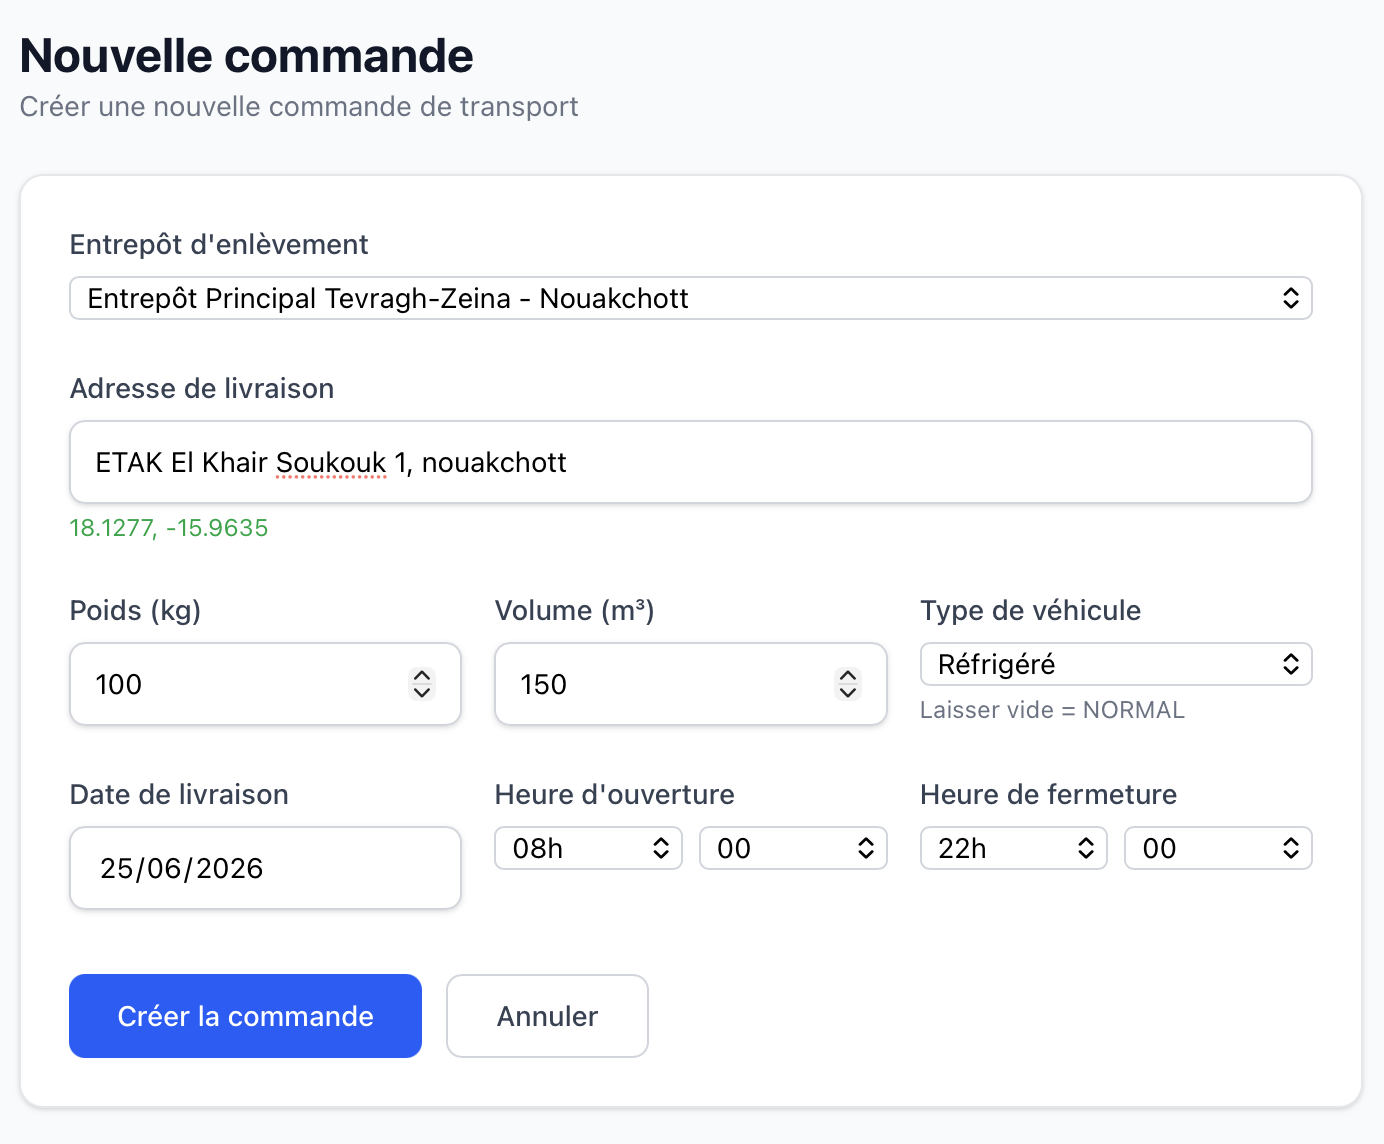
\includegraphics[width=0.9\textwidth]{capture/cree_commande.png}
  \caption{Interface de création de commande (Expéditeur)}
  \label{fig:ui-create-order}
\end{figure}

\paragraph{Liste des commandes.}
Tableau paginé avec filtres par statut et date. Chaque ligne affiche : adresse, date, statut (badge coloré), actions (détails, annuler si EN\_ATTENTE).

\subsection{Interface Dispatcheur}

\paragraph{Dashboard.}
Vue synthétique avec KPI en temps réel : nombre de commandes EN\_ATTENTE, tournées PLANIFIEES pour aujourd'hui, véhicules DISPONIBLES, taux OTD (On-Time Delivery) de la semaine. Graphique d'évolution des livraisons par jour (derniers 7 jours).

\begin{figure}[H]
  \centering
  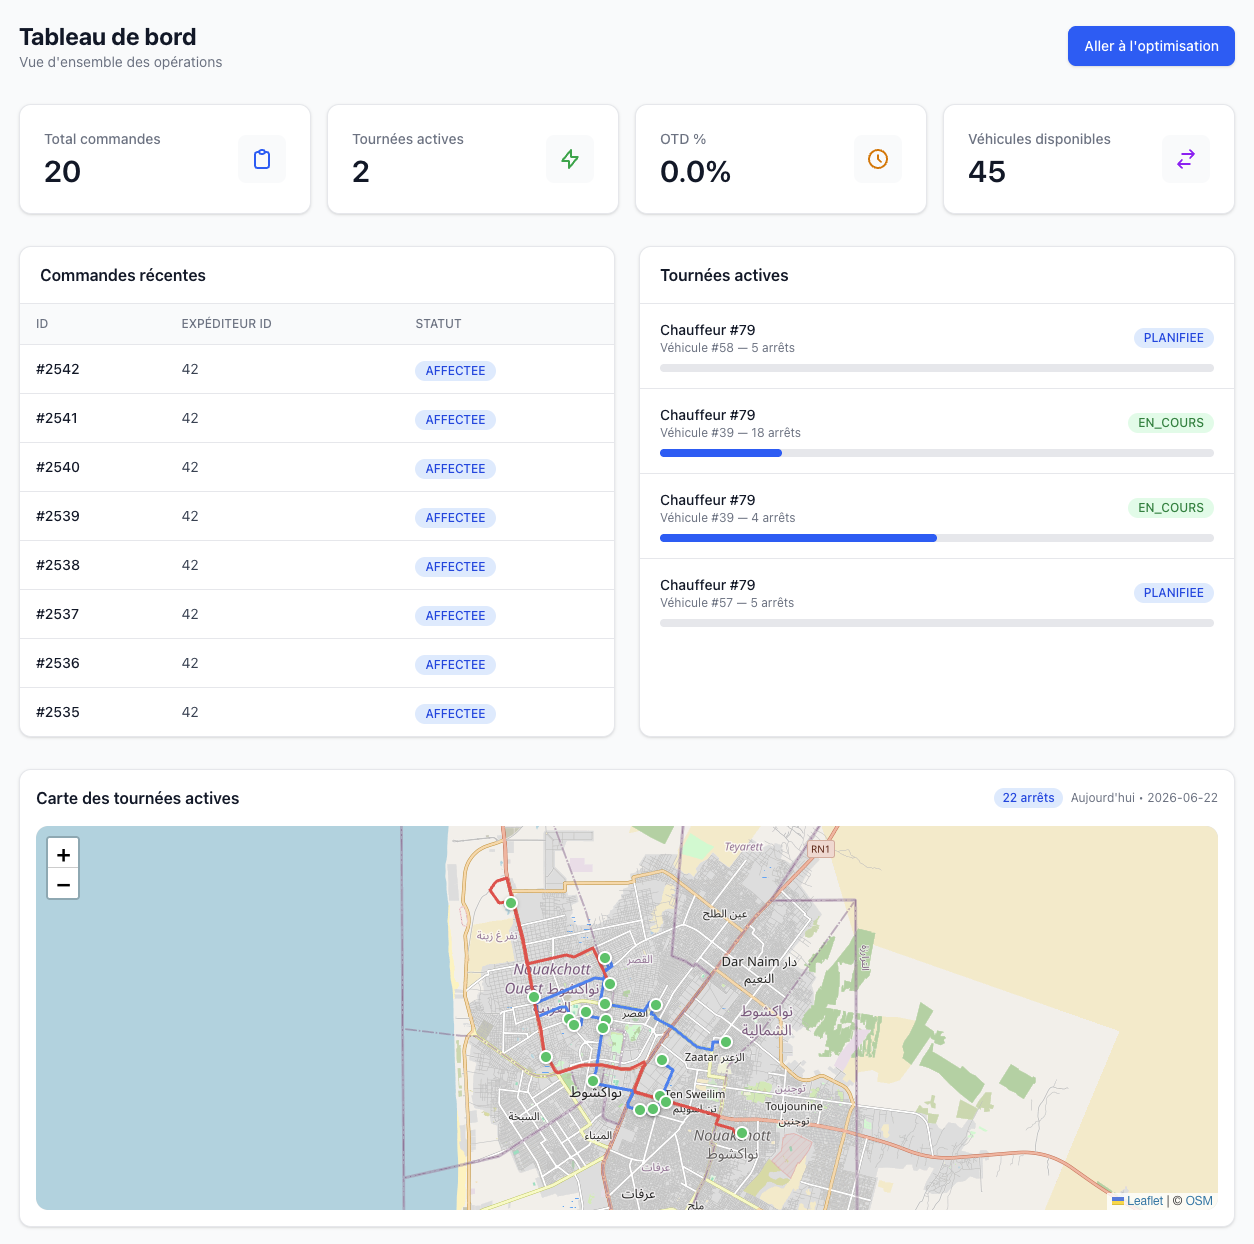
\includegraphics[width=\textwidth]{capture/dashboard.png}
  \caption{Dashboard principal (Dispatcheur)}
  \label{fig:ui-dashboard}
\end{figure}

\paragraph{Lancement d'optimisation.}
Interface en 3 étapes :
\begin{enumerate}[leftmargin=2.2em]
    \item Sélection des commandes (filtres par entrepôt, date, type).
    \item Sélection des véhicules disponibles.
    \item Validation et lancement. Affichage immédiat d'une barre de progression mise à jour via polling (toutes les 3s).
\end{enumerate}

Résultats affichés : distance totale, nombre de véhicules utilisés, nombre de commandes non servies, temps de calcul. Bouton pour visualiser les tournées créées sur carte.

\begin{figure}[H]
  \centering
  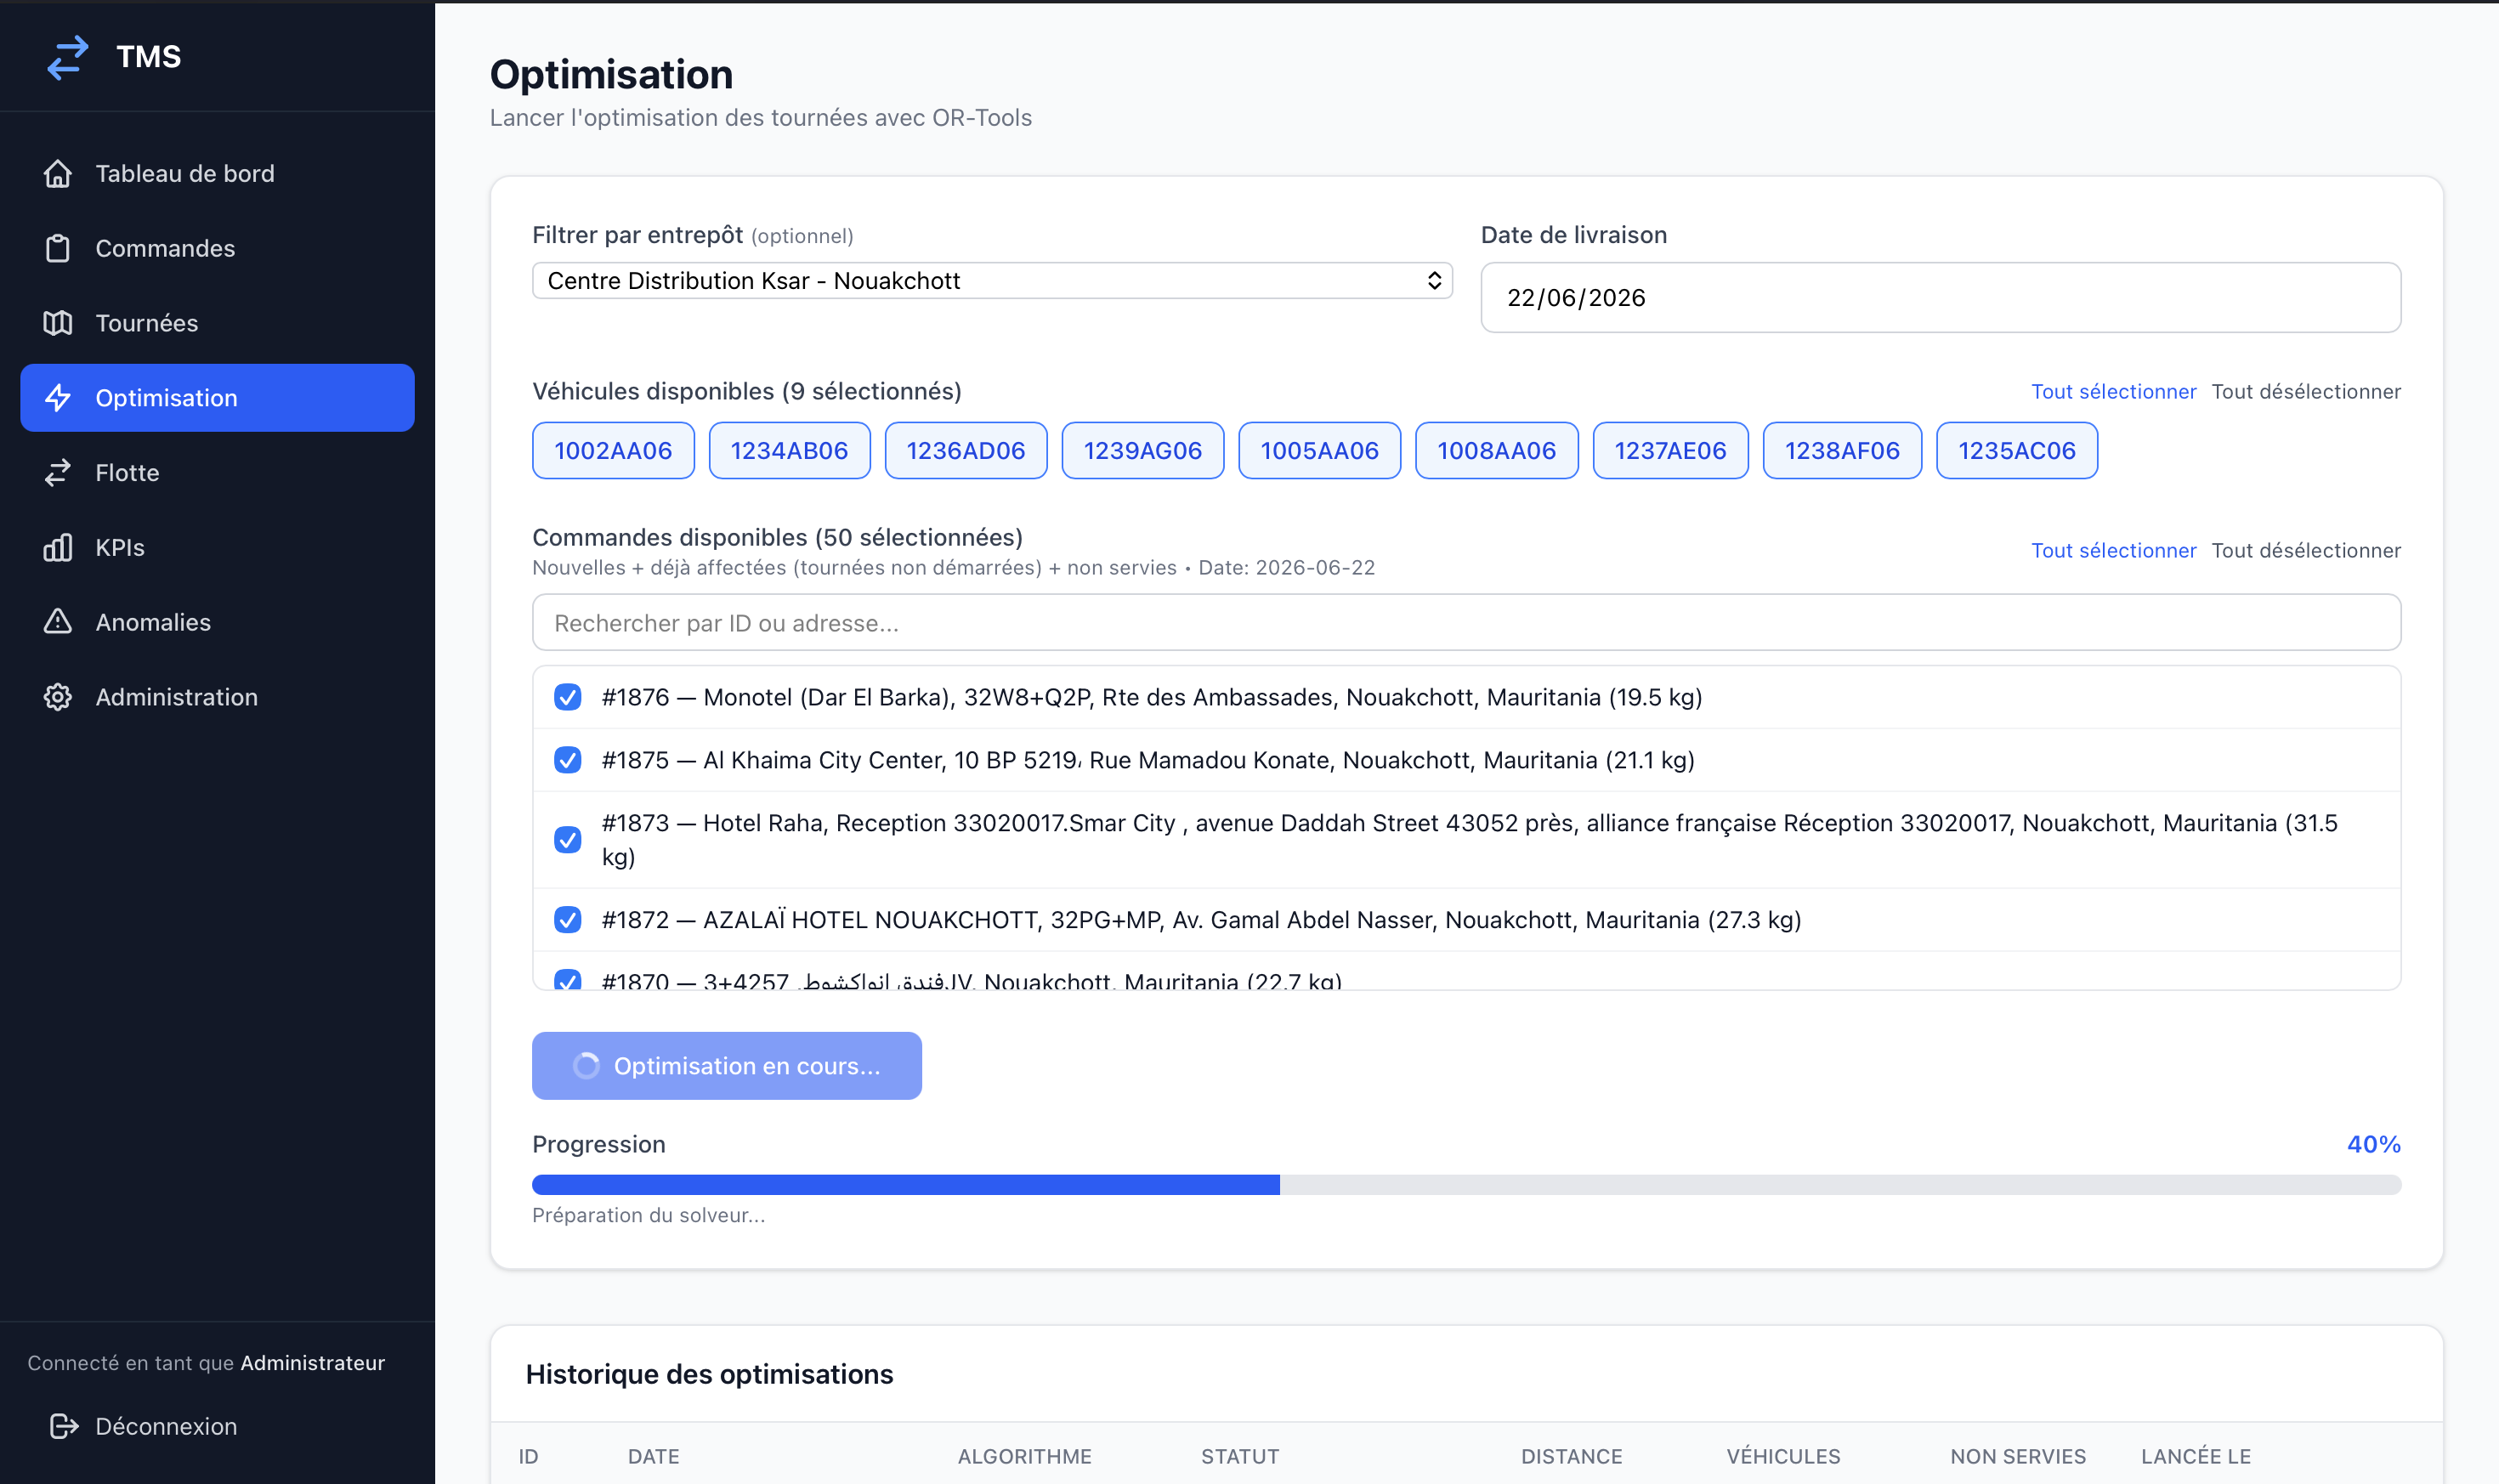
\includegraphics[width=\textwidth]{capture/optimisation.png}
  \caption{Interface d'optimisation avec barre de progression (Dispatcheur)}
  \label{fig:ui-optimisation}
\end{figure}

\paragraph{Visualisation des tournées.}
Carte Leaflet affichant tous les arrêts d'une tournée avec marqueurs colorés (EN\_ATTENTE : jaune, LIVREE : vert). Polyline reliant les arrêts dans l'ordre optimal. Panneau latéral listant les arrêts avec horaires prévus.

\begin{figure}[H]
  \centering
  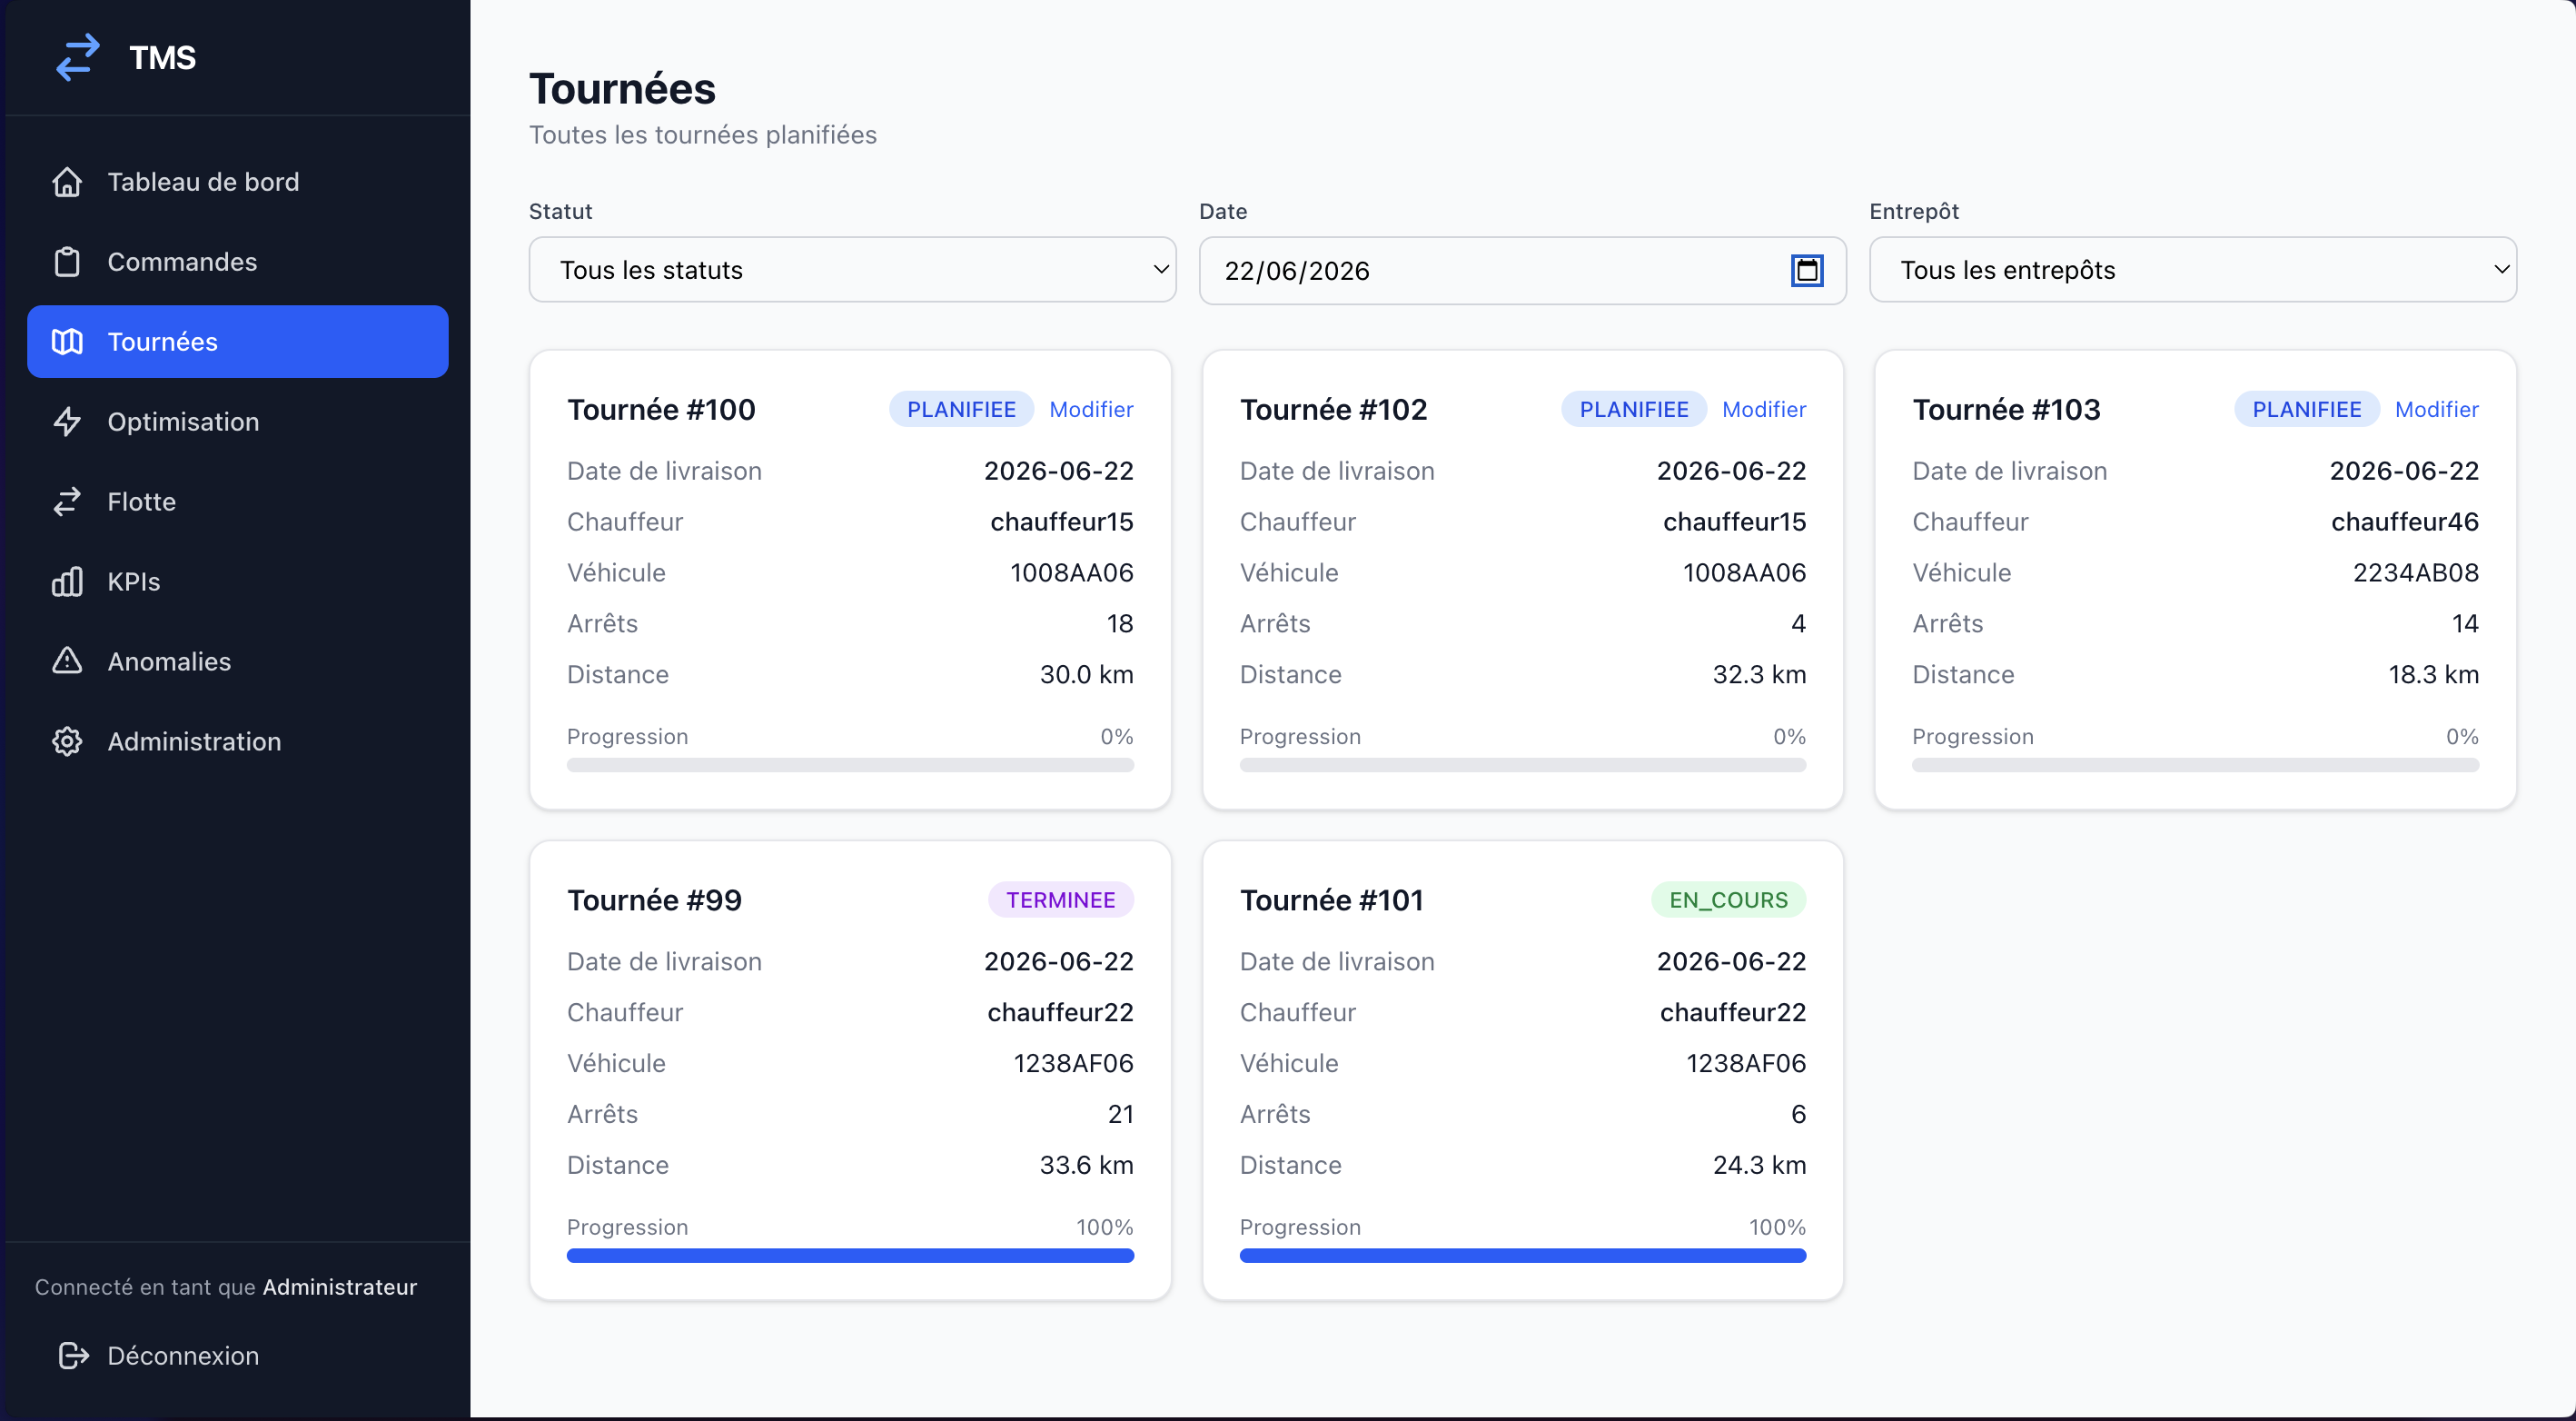
\includegraphics[width=\textwidth]{capture/tournees.png}
  \caption{Visualisation d'une tournée sur carte (Dispatcheur)}
  \label{fig:ui-tournee-map}
\end{figure}

\subsection{Interface Chauffeur}

\paragraph{Liste des tournées.}
Affichage des tournées assignées au chauffeur connecté, filtrées par date. Pour chaque tournée : véhicule, nombre d'arrêts, progression (\%).



\paragraph{Détail d'une tournée.}
Liste des arrêts triés par ordre de visite. Chaque arrêt affiche : adresse, horaire prévu, statut. Boutons d'action : "Démarrer tournée" (si PLANIFIEE), "Confirmer livraison" (si EN\_COURS), "Signaler anomalie".
\begin{figure}[H]
  \centering
  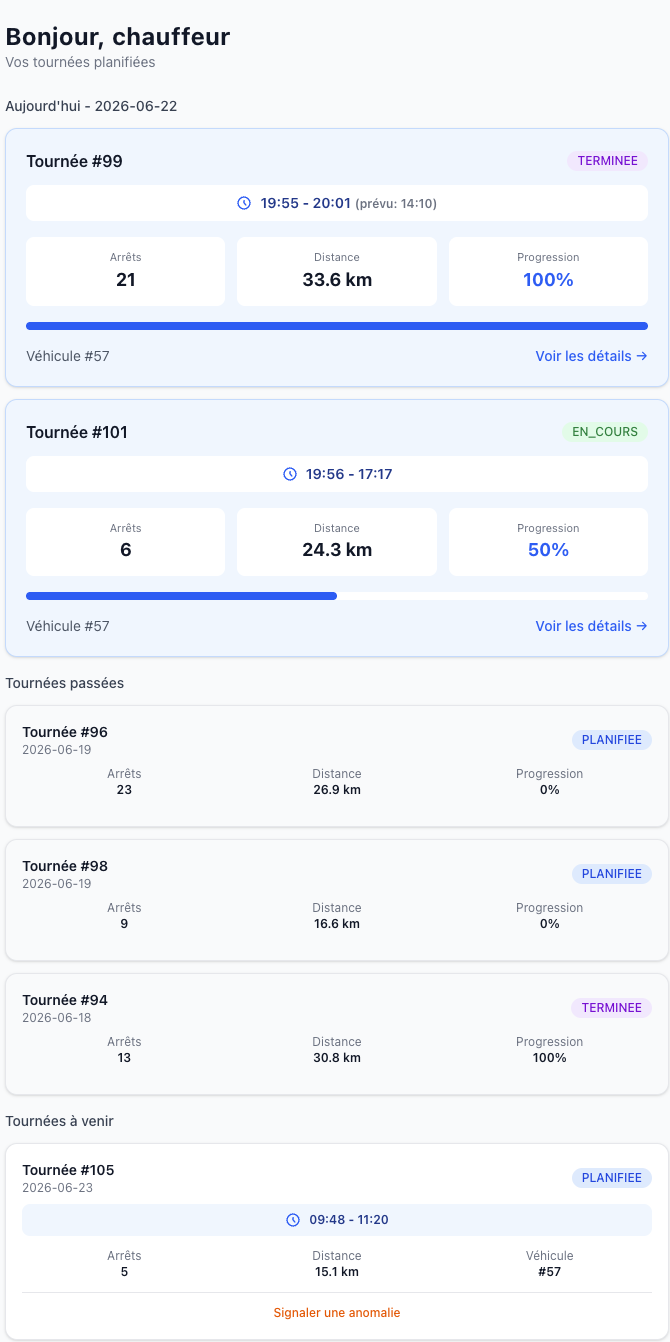
\includegraphics[height=0.75\textheight,keepaspectratio]{capture/chauffeur_dash.png}
  \caption{Dashboard des tournées (Chauffeur)}
  \label{fig:dash-chauffeur}
\end{figure}
\clearpage
\begin{figure}[p]
  \centering
  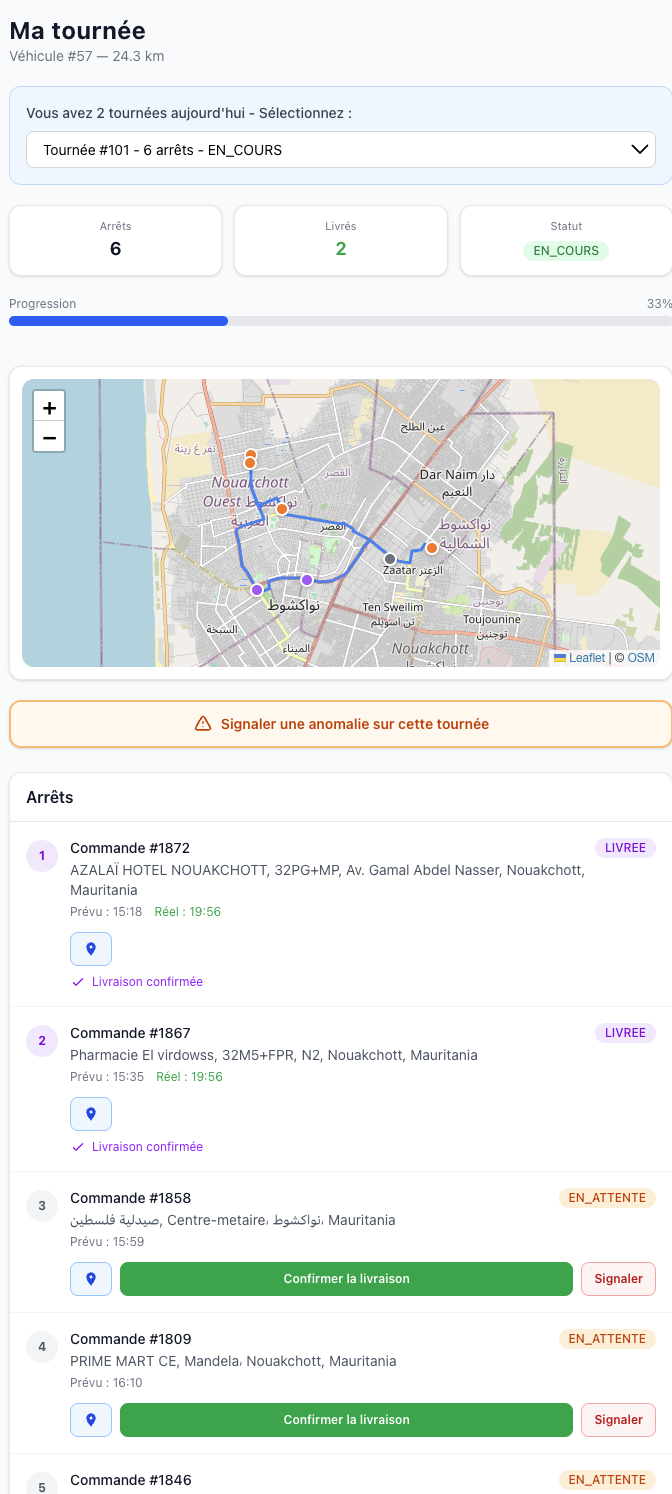
\includegraphics[height=0.82\textheight,keepaspectratio]{capture/chauffeur_tournee_du_jour.png}
  \caption{Interface d'exécution de tournée (Chauffeur)}
  \label{fig:ui-chauffeur}
\end{figure}
\clearpage

\paragraph{Confirmation de livraison.}
Clic sur "Confirmer" enregistre l'heure réelle et met à jour la progression. Notification toast : "Livraison confirmée. Prochain arrêt : [adresse]".

\subsection{Interface Administrateur}

\paragraph{Gestion des utilisateurs.}
CRUD complet : créer, modifier, activer/désactiver des comptes. Champs : nom, email, rôle, entrepôt de rattachement, statut (pour chauffeurs).

\paragraph{Gestion de la flotte.}
CRUD véhicules : immatriculation, capacités (poids, volume), type, entrepôt, statut.

\paragraph{Gestion des entrepôts.}
CRUD entrepôts : nom, ville, adresse, coordonnées GPS, horaires d'ouverture/fermeture.

\begin{figure}[H]
  \centering
  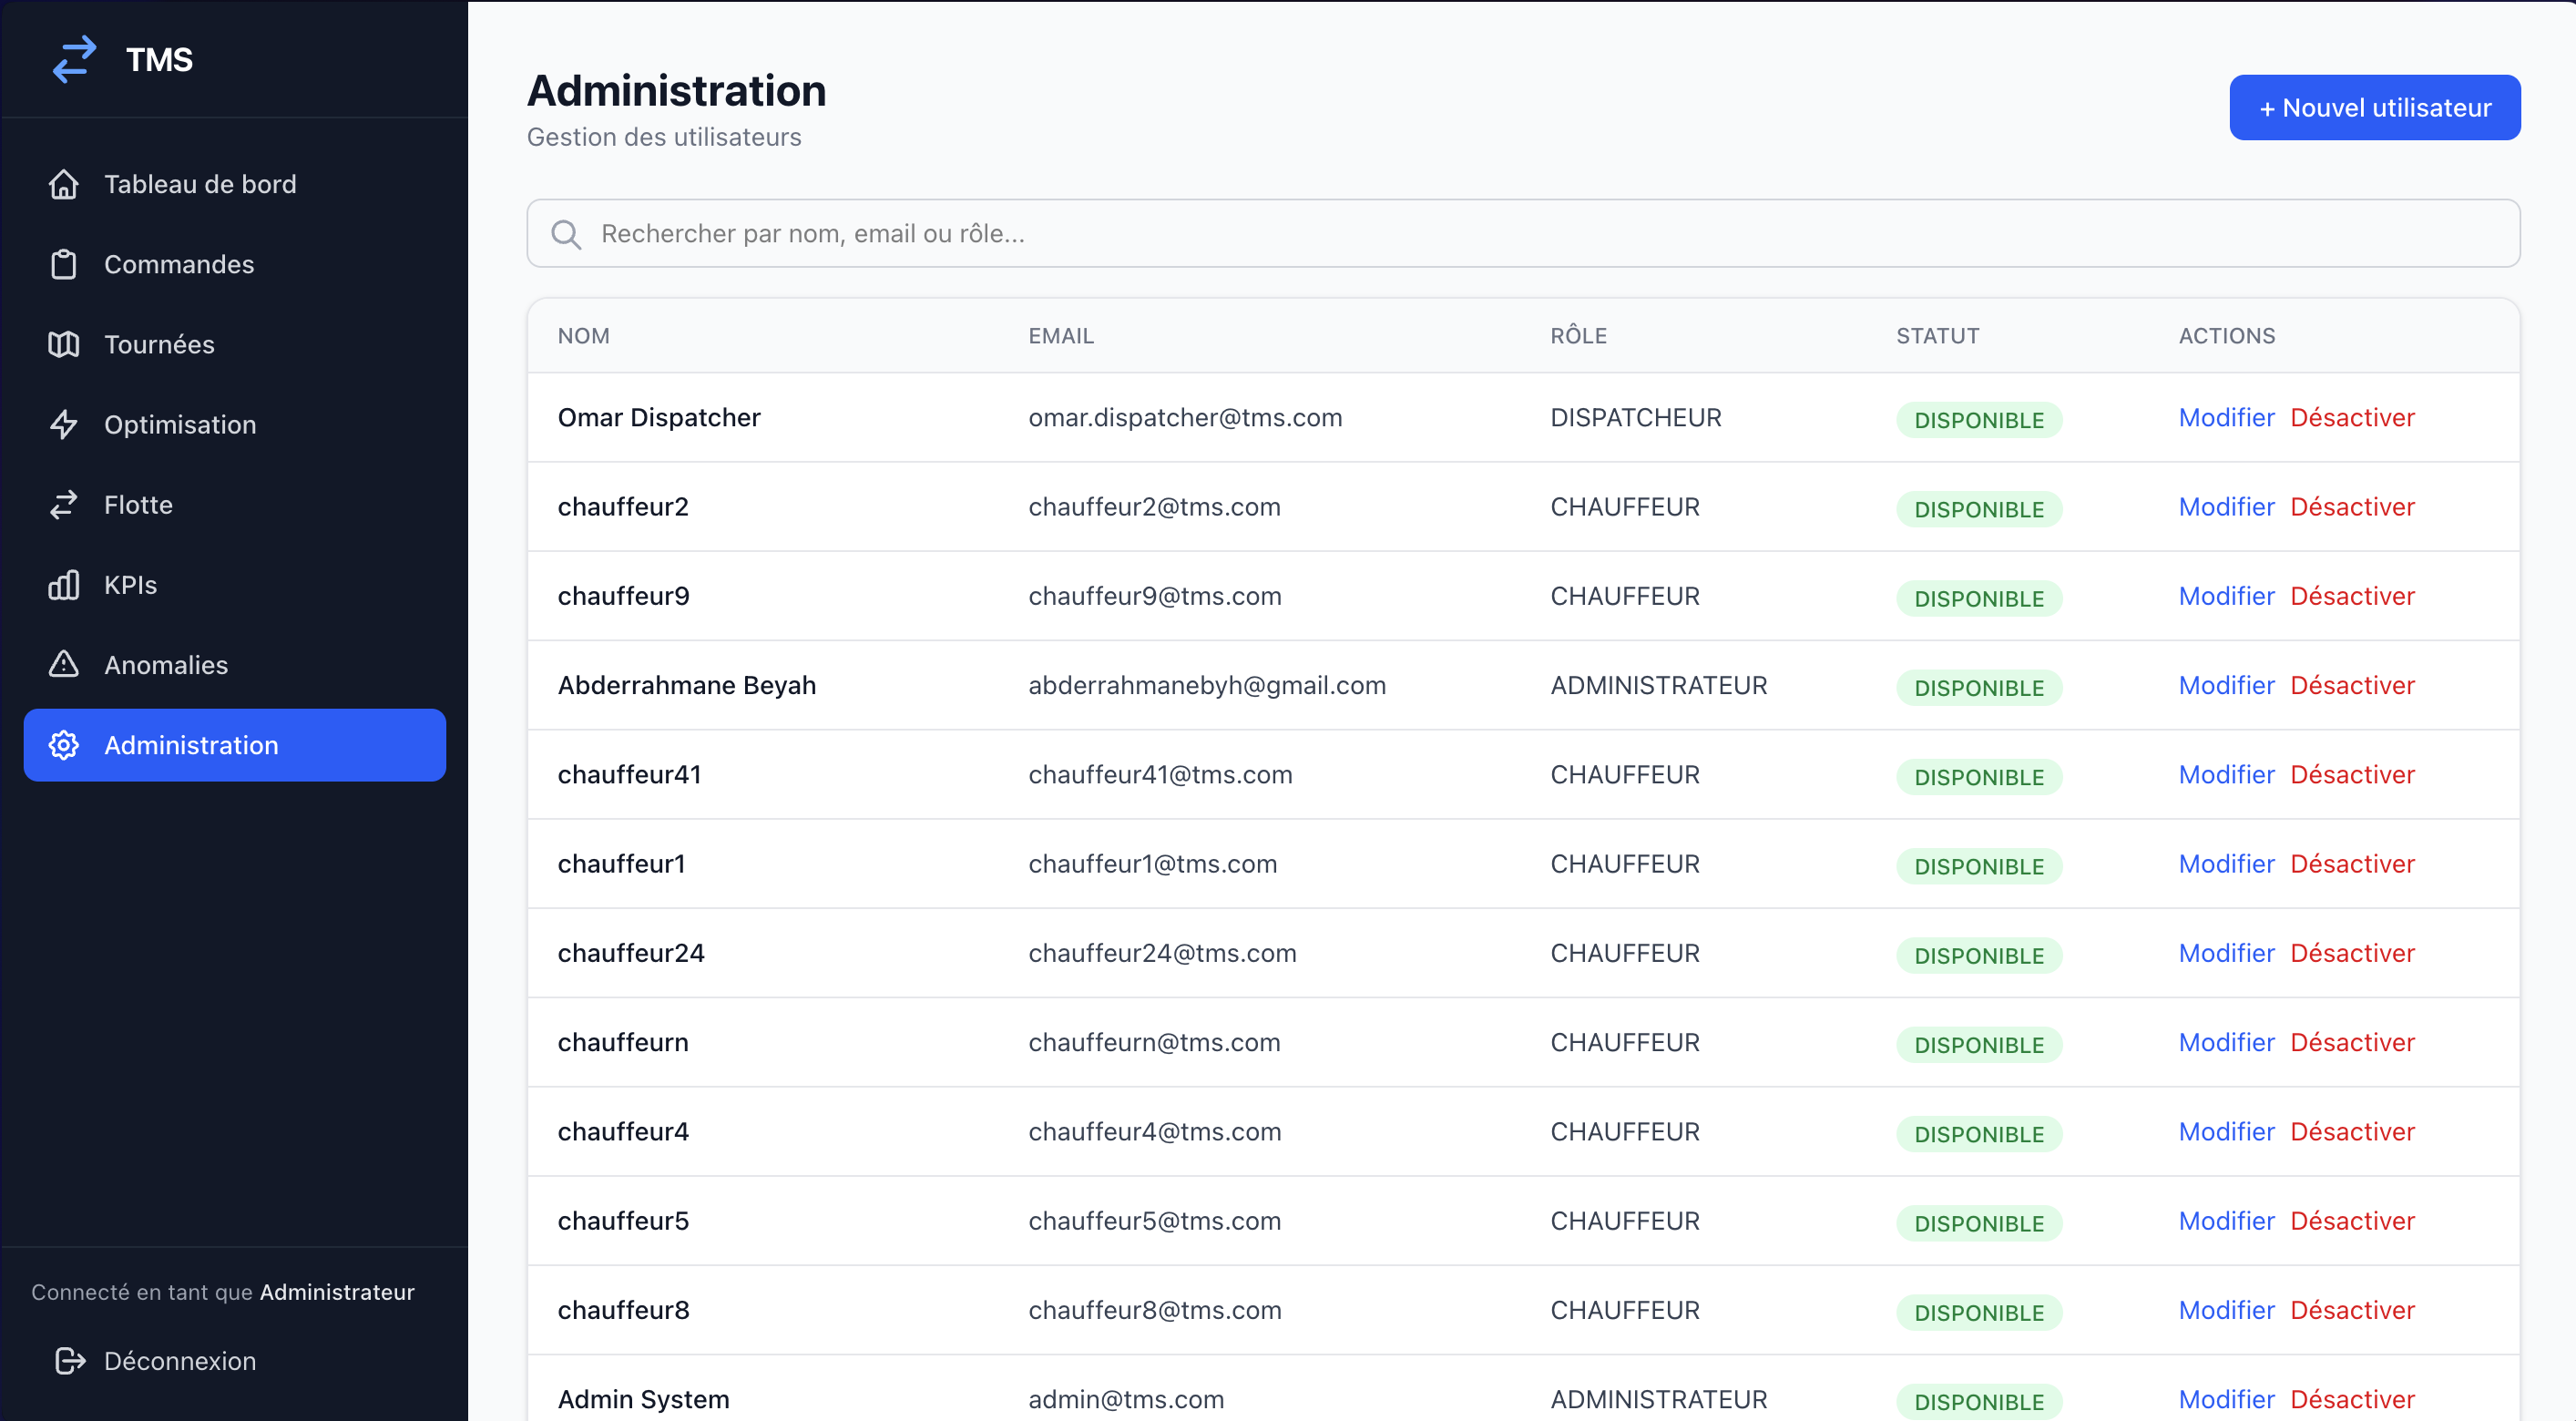
\includegraphics[width=\textwidth]{capture/administration.png}
  \caption{Interface d'administration (Administrateur)}
  \label{fig:ui-admin}
\end{figure}

\section{Déploiement}

\subsection{Conteneurisation Docker}

L'application complète est conteneurisée pour garantir la reproductibilité entre environnements. \texttt{docker-compose.prod.yml} orchestre 5 services :

\begin{itemize}[leftmargin=2.2em]
    \item \textbf{tms-db :} PostgreSQL 16 (port 5432), volume persistant pour les données.
    \item \textbf{tms-redis :} Redis 7 (port 6379), broker Celery.
    \item \textbf{tms-osrm :} Serveur OSRM prétraité avec données Mauritanie (port 5001).
    \item \textbf{tms-backend :} API FastAPI + Worker Celery (port 8000). Le script \texttt{start.sh} importe le dump SQL au premier lancement, puis démarre Celery et Uvicorn.
    \item \textbf{tms-frontend :} Nginx servant le build React (port 80).
\end{itemize}

\subsection{Déploiement sur VPS Hetzner}

Le système est déployé sur un VPS Hetzner (4 vCPU, 8GB RAM, Ubuntu 22.04) avec domaine pointant sur l'IP publique. Pipeline CI/CD via GitHub Actions : chaque push sur \texttt{main} déclenche une connexion SSH au VPS et la reconstruction des conteneurs Docker sur place (docker-compose build puis up).

\subsection{Environnements}

\textbf{Développement :} Docker Compose local (backend/.venv pour hot-reload Python, frontend npm dev server).

\textbf{Production :} Docker Compose production avec variables d'environnement (\texttt{.env.production}) : clés API, secrets JWT, URL de base de données.

\section{Évaluation des Performances}

\subsection{Méthodologie}

Les tests de performance ont été réalisés sur un MacBook Air M3 (16GB RAM) en environnement de développement, puis validés sur le VPS de production. 

\subsection{Temps de Calcul}

\begin{table}[H]
\centering
\begin{tabular}{lrr}
\toprule
\textbf{Taille du problème} & \textbf{Temps moyen (s)} & \textbf{Nb tests} \\
\midrule
4 commandes     & 30.1  & 1 \\
5 commandes     & 30.1  & 1 \\
8 commandes     & 30.2  & 1 \\
18 commandes    & 30.7  & 1 \\
22 commandes    & 60.7  & 1 \\
25 commandes    & 64.1  & 3 \\
28 commandes    & 62.5  & 1 \\
31 commandes    & 81.7  & 5 \\
37 commandes    & 124.2 & 1 \\
44 commandes    & 97.6  & 2 \\
46 commandes    & 61.4  & 2 \\
50 commandes    & 160.1 & 2 \\
57 commandes    & 198.8 & 1 \\
63 commandes    & 218.9 & 1 \\
94 commandes    & 180.7 & 1 \\
100 commandes   & 213.6 & 3 \\
106 commandes   & 262.5 & 1 \\
\bottomrule
\end{tabular}
\caption{Temps d'exécution moyen de l'optimisation (moyennes par taille sur 28 exécutions exploitables ; 31 tâches enregistrées au total)}
\label{tab:perf-temps}
\end{table}

\textbf{Méthodologie :} Données extraites de la table \texttt{tache\_optimisation} en production. Métriques mesurées : temps total (wall time), utilisation CPU (user+system time), augmentation mémoire (delta RSS du processus Celery).

\textbf{Observations :}
\begin{itemize}[leftmargin=2.2em]
    \item Les petits problèmes (< 20 commandes) se résolvent en ~30s (limite : 30s configurée).
    \item Les problèmes moyens (20-50 commandes) varient entre ~60s et ~160s selon les contraintes.
    \item Les grands problèmes (100-106 commandes) prennent ~3.5-4.5 minutes.
\end{itemize}


 \begin{figure}[H]
   \centering
   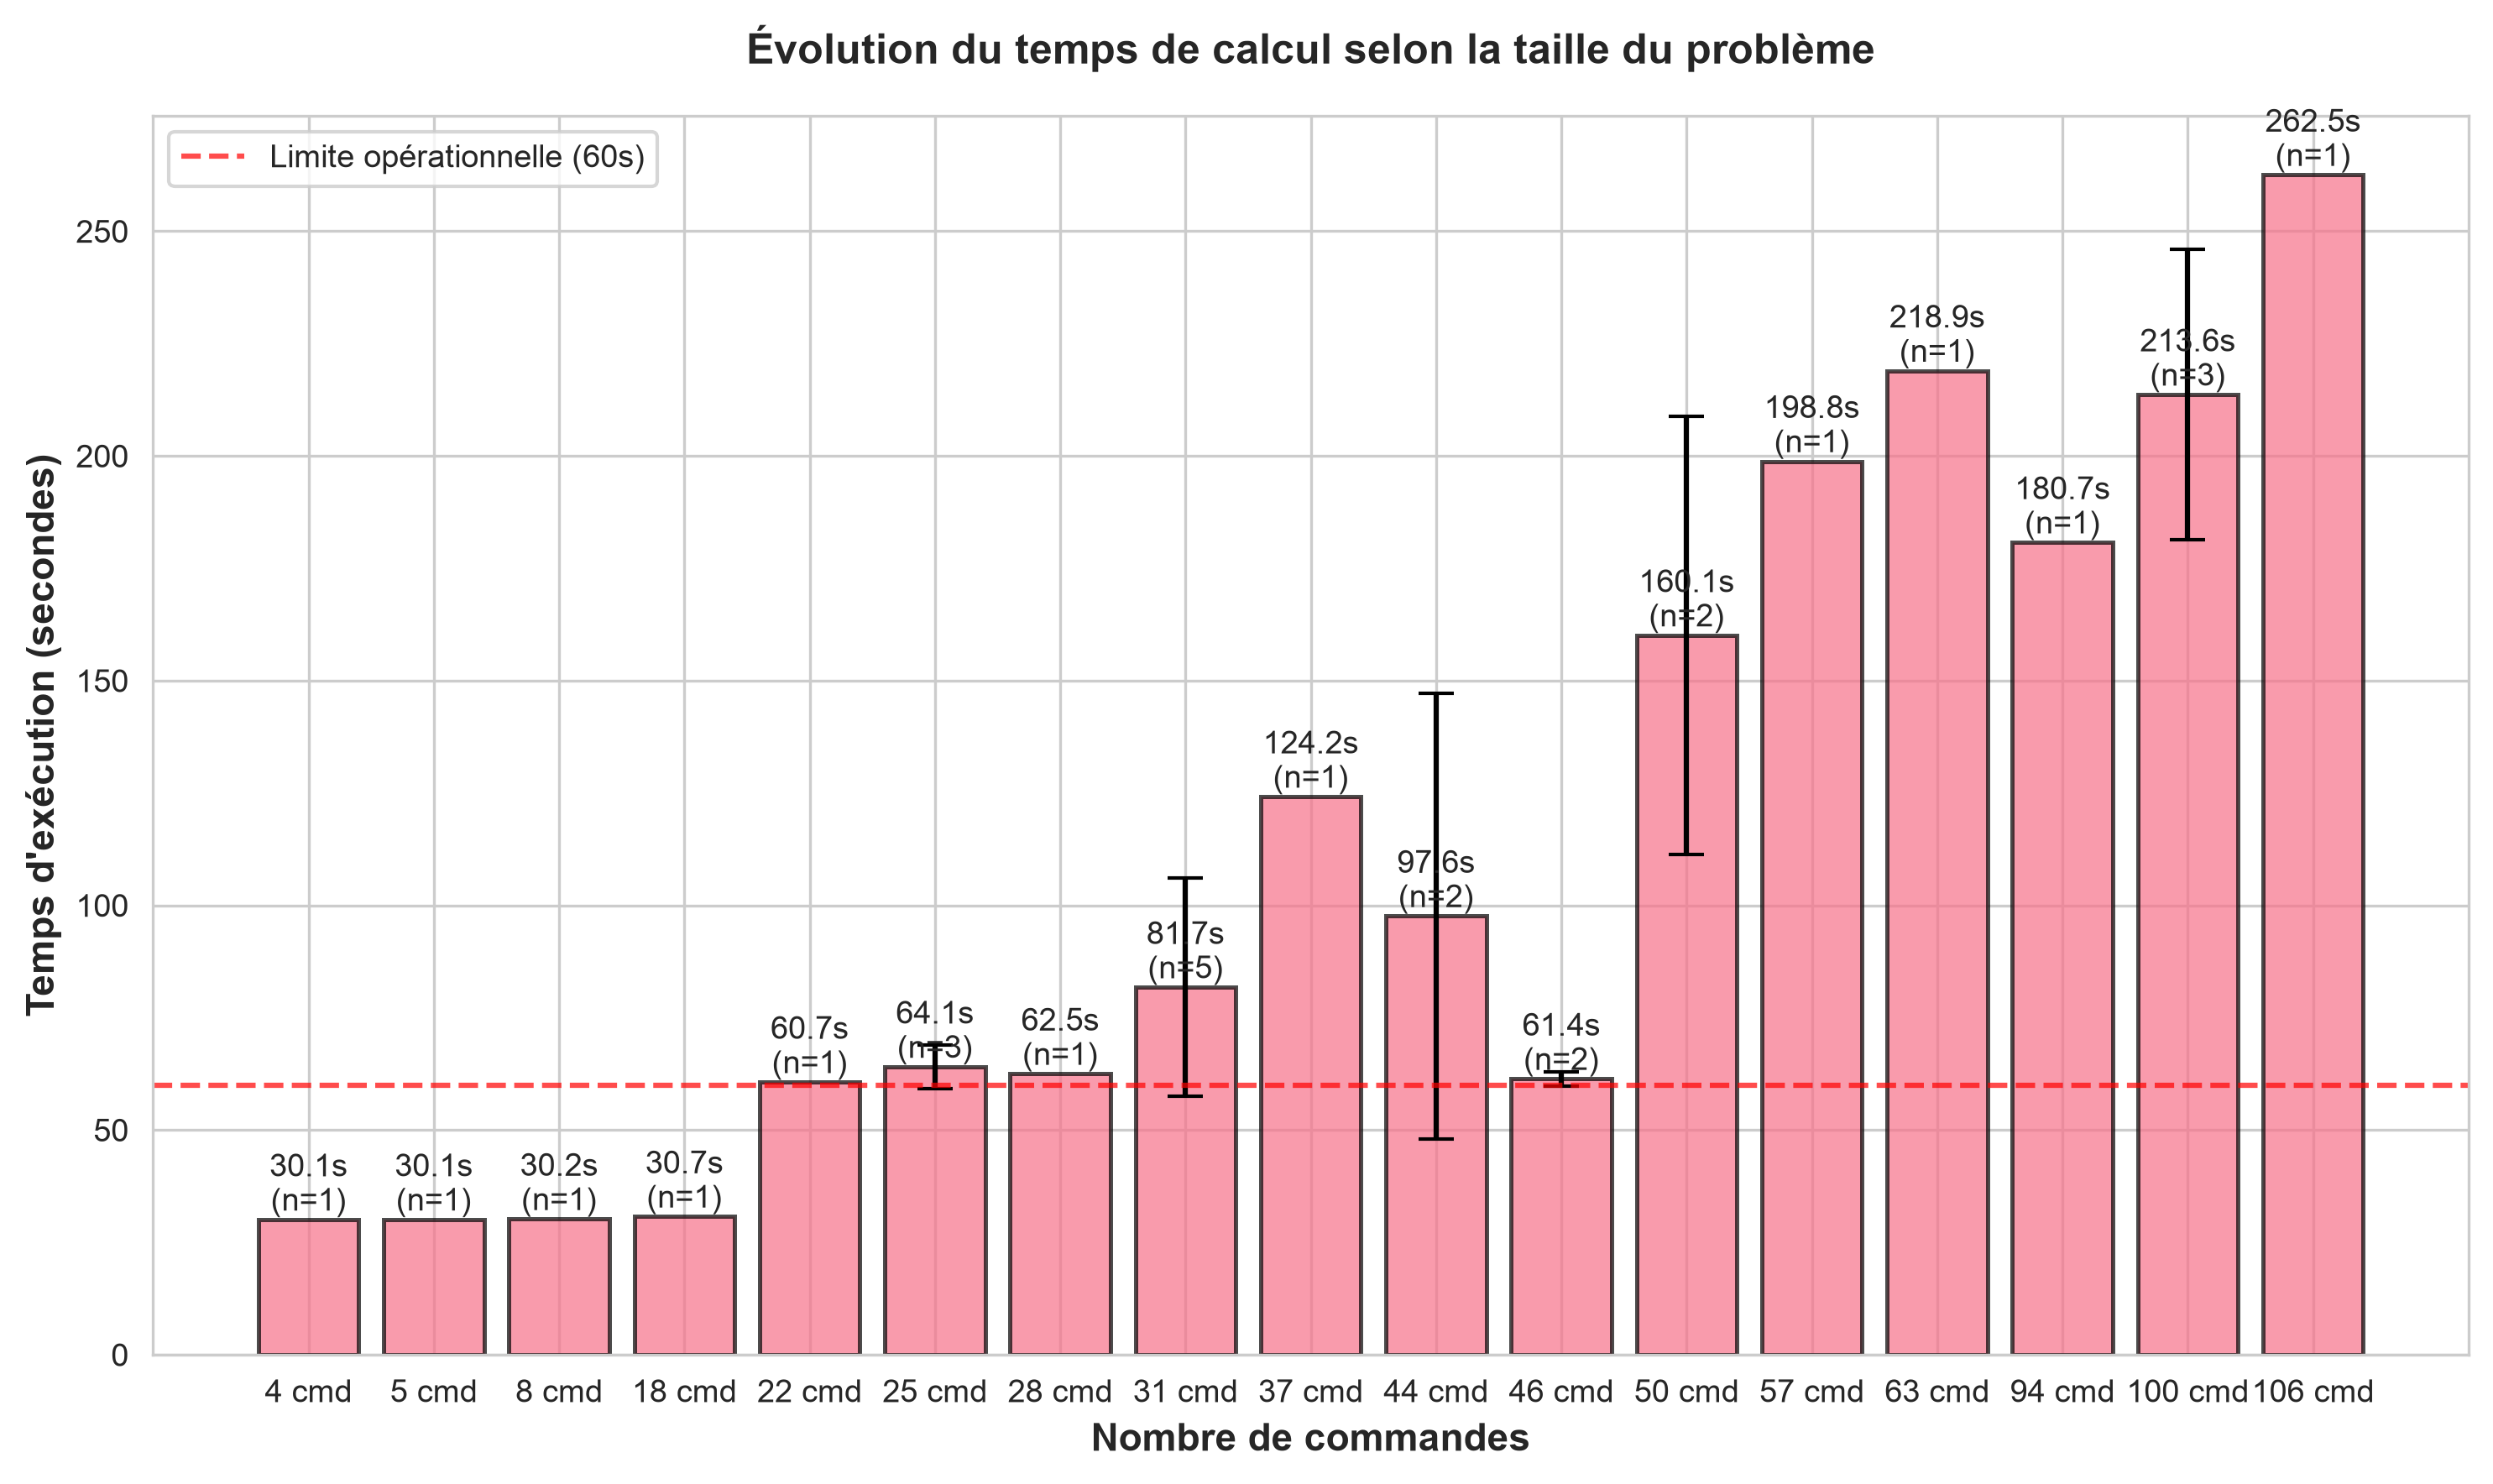
\includegraphics[width=0.9\textwidth]{benchmarks/computation_time.png}
   \caption{Évolution du temps de calcul selon la taille du problème}
   \label{fig:benchmark-time}
 \end{figure}

\subsection{Consommation Mémoire et CPU}

\begin{table}[H]
\centering
\begin{tabular}{lrr}
\toprule
\textbf{Taille} & \textbf{$\Delta$ RAM (MB)} & \textbf{CPU (\%)} \\
\midrule
P (< 20 cmd)  & 6.4 (max 12)  & 95-99  \\
M (20-50 cmd) & 3.8 (max 13)  & 90-96  \\
G (> 50 cmd)  & 6.7 (max 20)  & 83-98  \\
\bottomrule
\end{tabular}
\caption{Augmentation mémoire (delta RSS) et utilisation CPU pendant optimisation}
\label{tab:perf-ressources}
\end{table}

\textbf{Observations :}
\begin{itemize}[leftmargin=2.2em]
    \item La consommation RAM reste modérée ($<$ 600MB) même pour 50 commandes.
    \item Le CPU est pleinement utilisé (> 90\%) pour les grandes instances, justifiant l'asynchronisme Celery (pas de blocage de l'API).
\end{itemize}


 \begin{figure}[H]
   \centering
   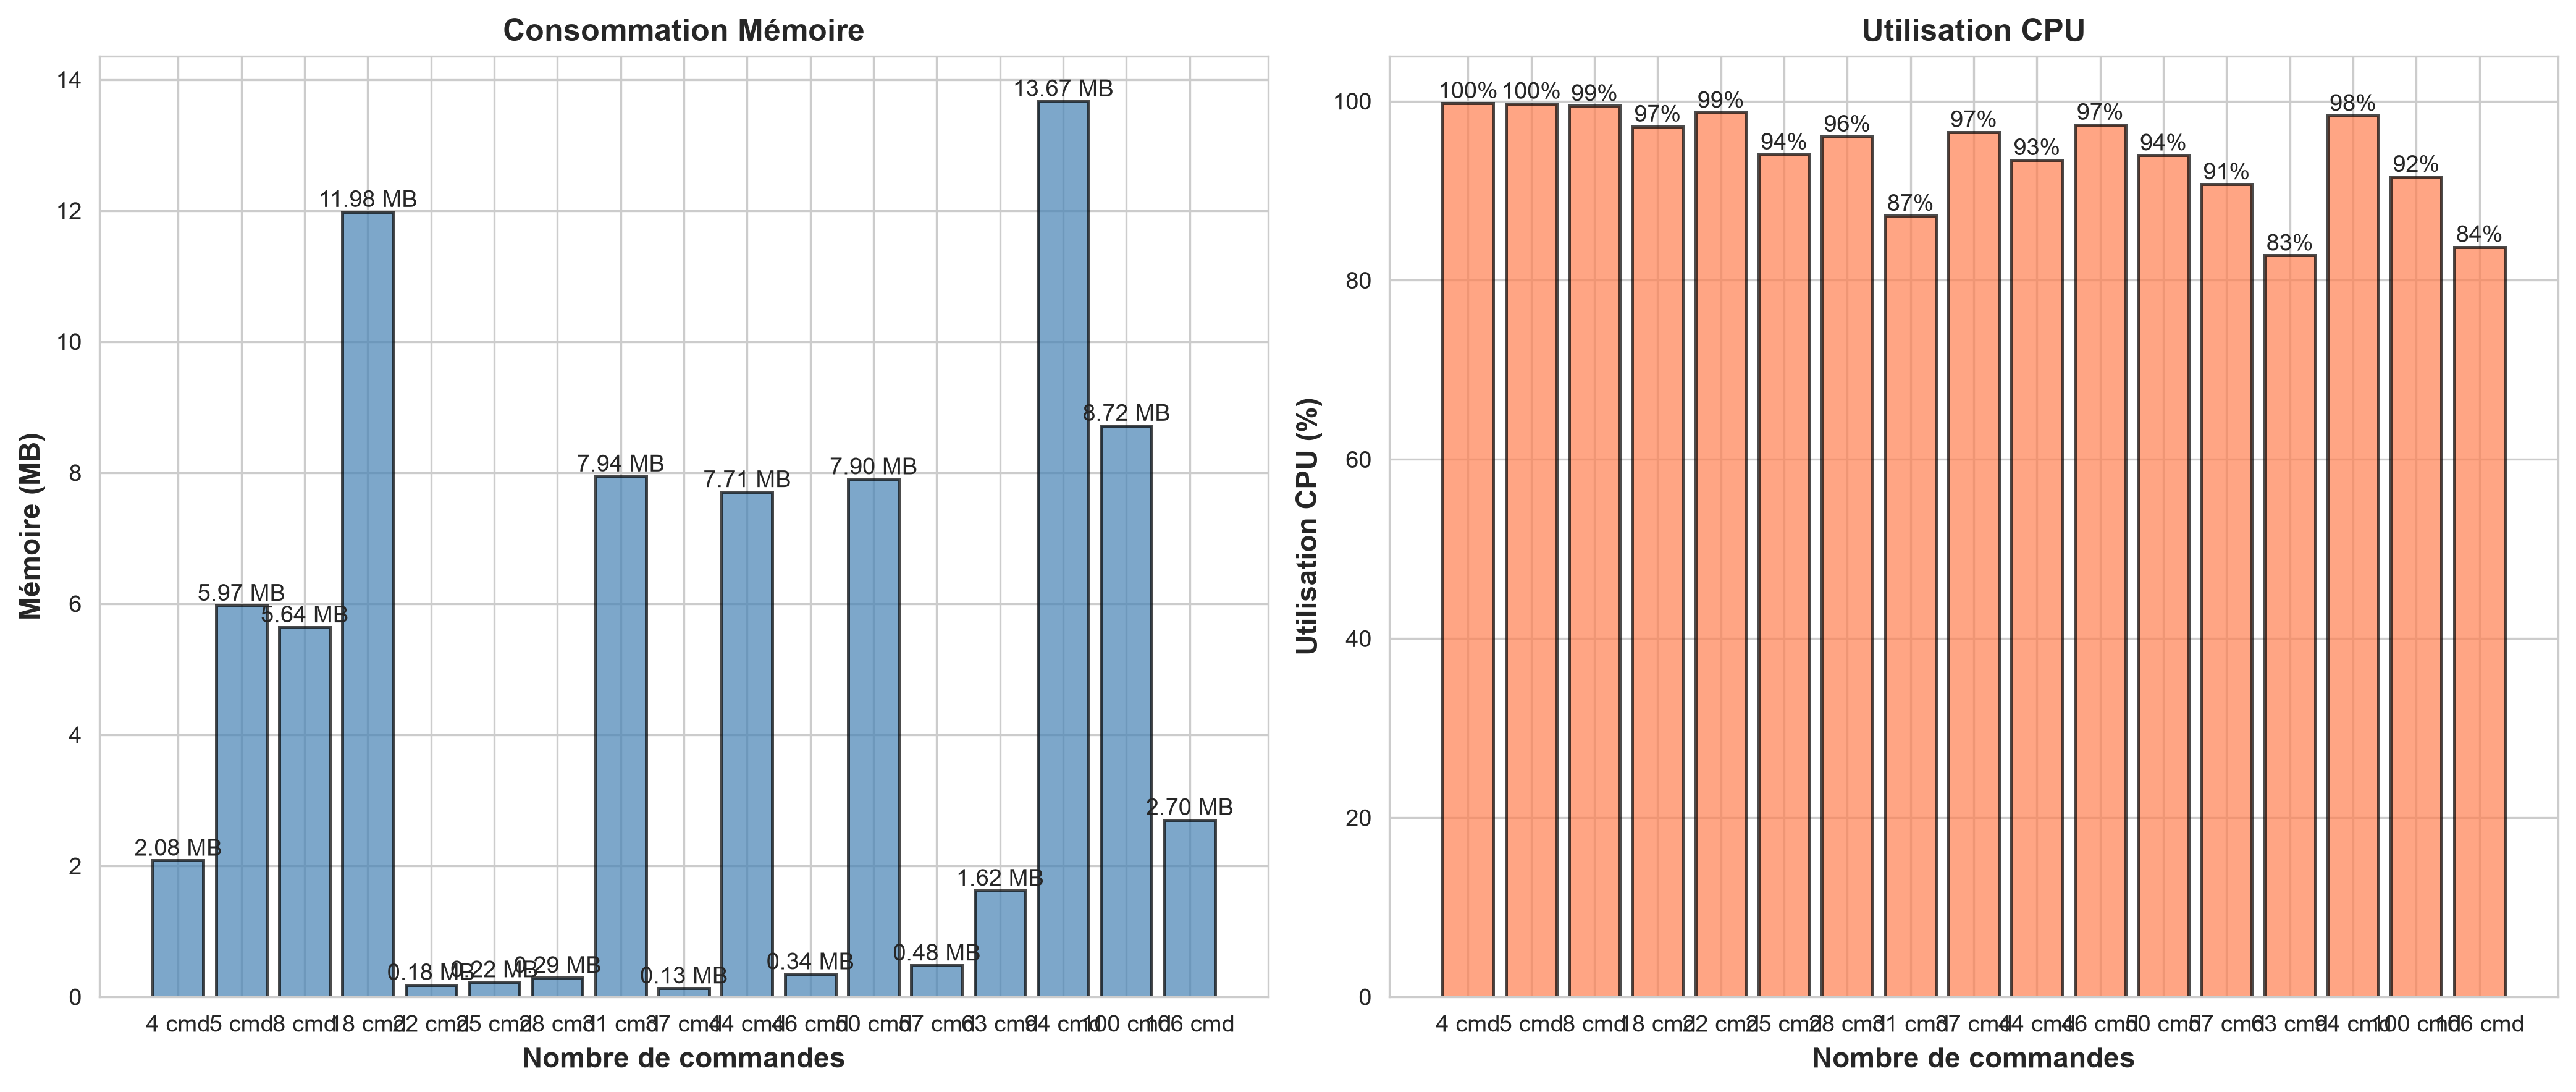
\includegraphics[width=0.9\textwidth]{benchmarks/resource_usage.png}
   \caption{Consommation mémoire et CPU selon la taille du problème}
   \label{fig:benchmark-resources}
 \end{figure}

\subsection{Qualité des Solutions}

Analyse de la qualité des solutions produites par OR-Tools sur des problèmes réels :

 \begin{figure}[H]
   \centering
   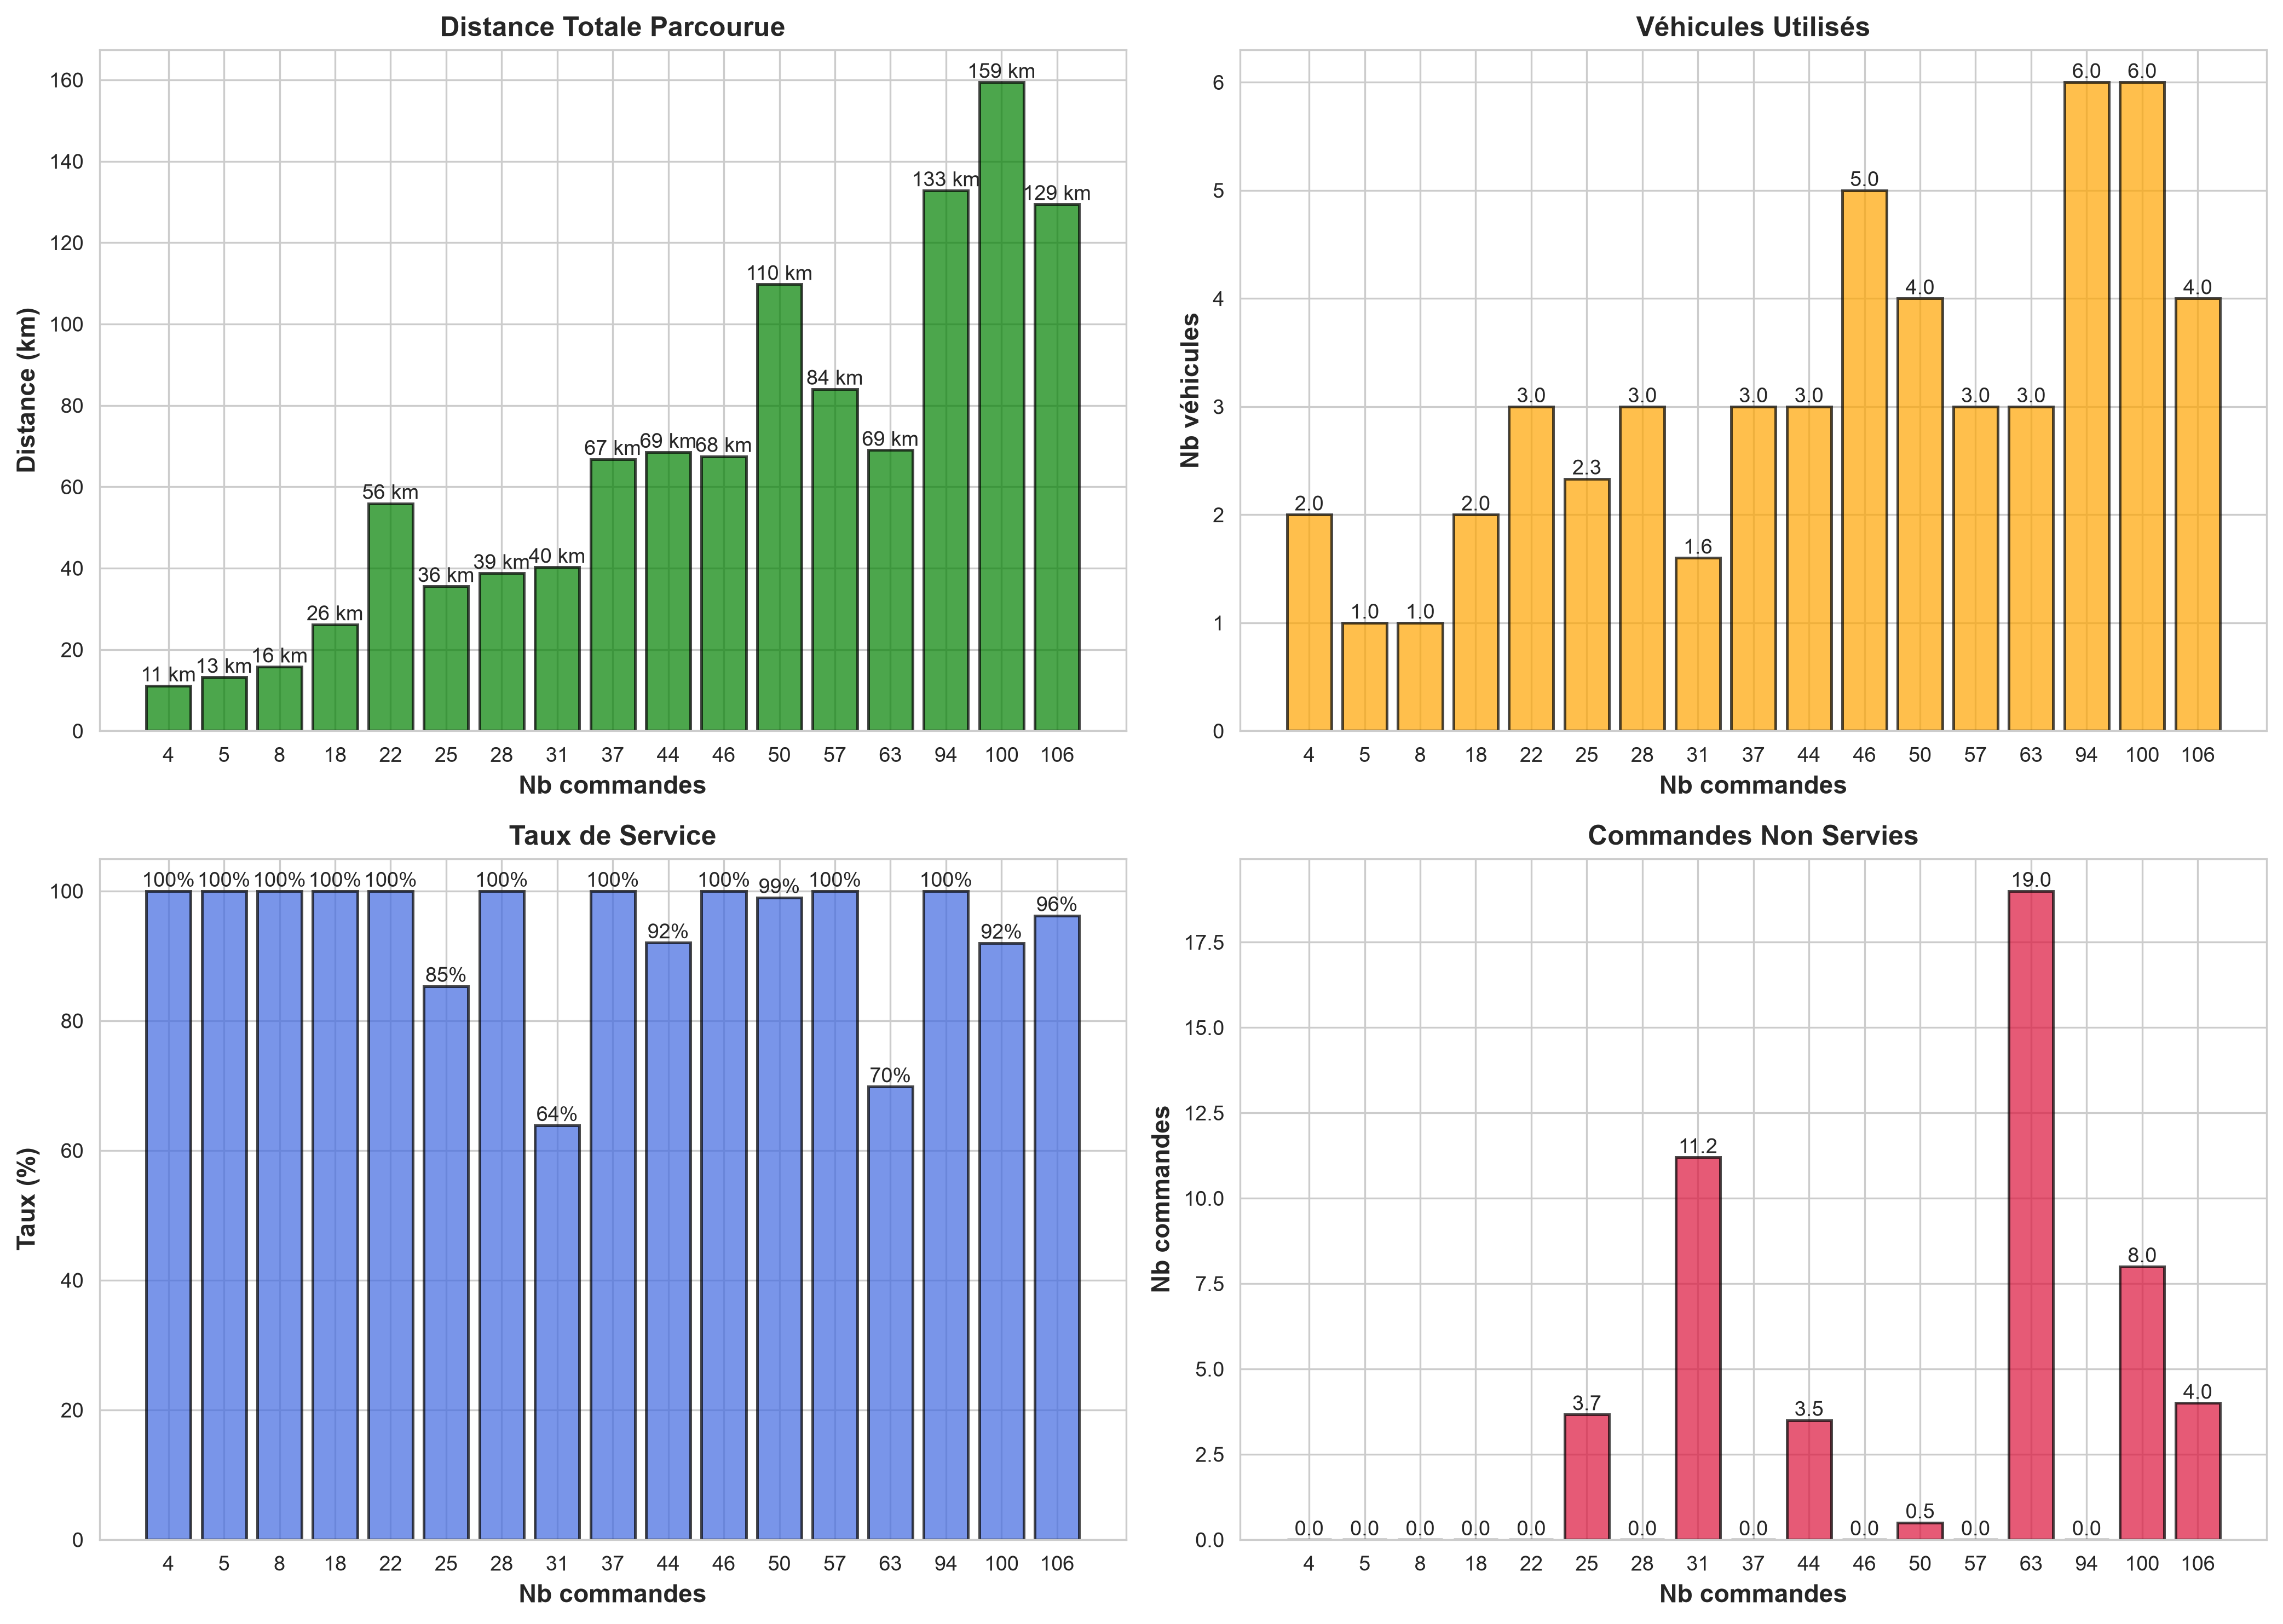
\includegraphics[width=0.9\textwidth]{benchmarks/solution_quality.png}
   \caption{Qualité des solutions OR-Tools : distance, véhicules, taux de service}
   \label{fig:benchmark-quality}
 \end{figure}

\textbf{Observations :} Le graphique montre les performances d'OR-Tools sur les optimisations réalisées : distances parcourues, nombre de véhicules utilisés, taux de service, et commandes non servies selon la taille du problème.


\subsection{Comparaison des Services de Routage}

\textit{Note : Tous les benchmarks ci-dessus utilisent OSRM comme service de routage (solution retenue pour la production). Le test ci-dessous compare OSRM au prototype initial utilisant Google Routes API v2 -- Compute Route Matrix.}

\subsubsection{Test comparatif : Google Routes API v2 vs OSRM}

Un test a été réalisé avec 100 commandes identiques pour comparer les performances de Google Routes API v2 -- Compute Route Matrix (utilisée dans le prototype initial) et OSRM (solution de production retenue). La comparaison porte sur le coût et le temps de calcul du routage ; les taux de livraison ne sont pas interprétés ici, car le nombre de chauffeurs disponibles n'était pas identique entre les deux exécutions.

\begin{table}[H]
\centering
\begin{tabular}{lrrr}
\toprule
\textbf{Métrique} & \textbf{Google Routes} & \textbf{OSRM} & \textbf{Gain} \\
\midrule
Temps total        & 1033s (17.2 min) & 251s (4.2 min) & \textbf{4.1×} \\
Coût par optimisation & 14\$          & 0\$            & 100\% \\
Erreurs 429 (rate limiting) & Oui    & Non            & -- \\
\bottomrule
\end{tabular}
\caption{Comparaison Google Routes API v2 vs OSRM (100 commandes identiques)}
\label{tab:benchmark-google-osrm}
\end{table}

\textbf{Analyse :} OSRM obtient un temps d'exécution 4.1× plus rapide (251s vs 1033s) et un coût nul. L'écart mesuré s'explique principalement par l'overhead d'accès au service cloud et par les interruptions dues aux erreurs 429 (rate limiting) observées avec Google. La qualité des solutions n'est pas comparée ici, car les ressources disponibles (notamment les chauffeurs) différaient entre les deux exécutions.

Le ralentissement de Google ne provient pas de l'algorithme de routage lui-même, mais de l'overhead d'accès au service cloud : latence réseau ($\sim$150ms par requête), authentification, chunking (limite de 25 origines × 25 destinations par appel, soit jusqu'à 25 appels pour 100 commandes + dépôt), et délais obligatoires entre requêtes (2s) pour éviter le rate limiting. OSRM, hébergé localement en Docker, présente une latence < 1ms et aucune limitation.

Ces résultats ont motivé le choix d'OSRM pour la production. Pour les cas nécessitant des données de trafic temps-réel ou des polylines GPS précises (affichage sur l'interface chauffeur), l'architecture peut être enrichie par des appels ponctuels à Google Directions API \emph{après} l'optimisation, sur les K tournées finales uniquement (où K $\ll$ N), réduisant ainsi les coûts de 99\% (14\$ $\rightarrow$ 0.025\$) tout en conservant les avantages de Google.

\subsection{Scalabilité}

Tests de charge réalisés sur l'API avec Apache Bench (outil de benchmarking HTTP). Chaque endpoint a été testé avec des requêtes concurrentes pour évaluer le débit maximum et la latence moyenne.

\begin{table}[H]
\centering
\small
\begin{tabular}{lrrr}
\toprule
\textbf{Endpoint} & \textbf{Débit (req/s)} & \textbf{Latence (ms)} & \textbf{Charge} \\
\midrule
GET /anomalies          & 668 & 150 & 100 concurrentes \\
GET /chauffeurs         & 468 & 214 & 100 concurrentes \\
GET /vehicules          & 456 & 220 & 100 concurrentes \\
GET /commandes          & 248 & 403 & 100 concurrentes \\
GET /optimisation/historique & 209 & 479 & 100 concurrentes \\
GET /kpis/otd           & 79  & 126 & 10 concurrentes  \\
GET /kpis/utilisation   & 62  & 162 & 10 concurrentes  \\
GET /tournees           & 53  & 188 & 10 concurrentes  \\
\bottomrule
\end{tabular}
\caption{Performance de l'API sous charge (Apache Bench, 0\% échecs)}
\label{tab:api-scalability}
\end{table}

\textbf{Résultats :} Les endpoints simples (anomalies, chauffeurs, véhicules) atteignent 450-670 req/s avec latence < 250ms. Les endpoints complexes avec jointures ou calculs (commandes, KPIs) maintiennent 50-250 req/s avec latence < 500ms. Le système supporte largement la charge attendue (< 50 utilisateurs simultanés en production).

\section{Conclusion}

Ce chapitre a détaillé la réalisation du système TMS, de la sélection de la pile technologique au déploiement en production. L'évaluation comparative des services de routage montre qu'OSRM réduit fortement le temps et le coût de construction des matrices (251s contre 1033s avec Google Routes API v2, coût 0\$ contre 14\$ par optimisation), ce qui a motivé le choix d'OSRM pour la production.

L'implémentation du moteur d'optimisation traduit les contraintes mathématiques du chapitre 2 en code opérationnel. L'utilisation d'OSRM pour le calcul matriciel élimine la latence réseau, le rate limiting et les coûts d'API observés avec Google Routes API v2.

Les interfaces utilisateur sont adaptées à chaque rôle (expéditeur : création de commandes ; dispatcheur : optimisation et KPIs ; chauffeur : exécution des tournées ; administrateur : gestion des utilisateurs et de la flotte). Les tests de charge montrent que l'API supporte 50-670 req/s selon la complexité des endpoints, avec 0\% d'échecs.

Le système est déployé sur serveur VPS et accessible via navigateur web. Le déploiement Docker assure la reproductibilité entre environnements.

\chapter*{Conclusion Générale}
\addcontentsline{toc}{chapter}{Conclusion Générale}

\section*{Synthèse des contributions}

Ce projet de fin d'études a permis de concevoir, développer et déployer un Système de Gestion du Transport (TMS) pour la planification des tournées de livraison dans le contexte mauritanien. La réalisation s'articule autour de trois contributions :

\paragraph{Contribution algorithmique et mathématique.} Nous avons formalisé le problème de tournées comme un VRPTW multi-contraint avec capacités multiples (poids, volume), fenêtres de temps strictes, types de véhicules hétérogènes, et support du multi-trajets. L'implémentation du solveur basé sur OR-Tools et la métaheuristique GLS obtient un taux de service > 85\% en 30s-4.5min lorsque les ressources disponibles sont suffisantes, tandis que les scénarios limités en véhicules ou chauffeurs mettent en évidence les commandes non servies. L'utilisation d'OSRM comme service de routage élimine la latence réseau, le rate limiting, et les coûts observés avec Google Routes API v2.

\paragraph{Contribution technique.} L'architecture mise en place (backend FastAPI, worker Celery asynchrone, frontend React, base PostgreSQL, OSRM auto-hébergé) sépare les responsabilités : l'API répond immédiatement (< 1s) lors du lancement d'une optimisation, tandis que le worker Celery exécute le calcul en arrière-plan (30s-4.5min).

Le contrôle d'accès par rôle limite les actions selon l'utilisateur : l'expéditeur crée des commandes, le dispatcheur lance les optimisations, le chauffeur confirme les livraisons, l'administrateur gère les utilisateurs. Les tests de charge montrent que l'API supporte 50-670 req/s selon la complexité des endpoints, avec 0\% d'échecs.

\paragraph{Contribution fonctionnelle.} Le système couvre le cycle de vie de la livraison : création des commandes (avec géocodage automatique), optimisation des tournées (sélection des commandes et véhicules, lancement asynchrone, suivi de progression), exécution terrain (confirmation des livraisons par les chauffeurs), et tableaux de bord KPI (taux de livraison à l'heure, utilisation de la flotte).

Chaque rôle dispose d'une interface spécifique : formulaire de création pour l'expéditeur, interface d'optimisation et carte pour le dispatcheur, liste des arrêts pour le chauffeur, gestion des utilisateurs pour l'administrateur.

\section*{Validation des objectifs}

Les objectifs fixés en introduction ont été atteints :

\begin{itemize}[leftmargin=2.2em]
    \item \textbf{Modélisation mathématique :} Le VRPTW est formellement défini avec toutes ses contraintes, et la complexité NP-difficile justifie le recours aux métaheuristiques.

    \item \textbf{Implémentation opérationnelle :} Le solveur est intégré dans une application web complète, avec exécution asynchrone et suivi de progression.

    \item \textbf{Intégration cartographique :} L'utilisation d'OSRM avec les données OSM de Mauritanie fournit des distances et temps routiers cohérents avec le réseau OpenStreetMap disponible, critiques pour la validité des solutions.

    \item \textbf{Performance :} Les temps de calcul respectent les contraintes opérationnelles (environ 2.5-4.5 min pour 50-100+ commandes), et l'augmentation mémoire durant l'optimisation reste faible (< 20 MB, métrique : delta RSS du processus Celery).

    \item \textbf{Déploiement :} Le système est opérationnel en production sur serveur VPS, accessible via navigateur web standard.
\end{itemize}

\section*{Limites et défis rencontrés}

Plusieurs limites et défis ont marqué le développement :

\paragraph{Qualité des données cartographiques.} Les données OpenStreetMap pour la Mauritanie présentent des lacunes (routes manquantes, adresses incomplètes), ce qui affecte la précision du géocodage et du routage dans certaines zones périphériques.

\paragraph{Complexité algorithmique.} Malgré l'utilisation d'une métaheuristique avancée, le VRPTW reste NP-difficile. Pour des instances très contraintes (nombreuses fenêtres strictes incompatibles), le solveur peut ne pas trouver de solution réalisable ou laisser certaines commandes non affectées.

\paragraph{Multi-trajets.} L'implémentation actuelle fonctionne en deux phases séquentielles. Phase 1 : optimisation avec les véhicules sélectionnés selon les types de commandes. Phase 2 : les commandes non servies sont re-optimisées, et les chauffeurs peuvent changer de véhicule (exemple : utiliser un véhicule NORMAL en Phase 1, puis un REFRIGERE en Phase 2 après retour au dépôt).

Cette approche séquentielle améliore le taux de service mais ne garantit pas l'optimalité globale (une optimisation conjointe des deux phases pourrait trouver une meilleure solution).

\paragraph{Scalabilité à très grande échelle.} Les tests ont été effectués avec jusqu'à 50-100 commandes. Au-delà de 200 commandes, il faudrait envisager des techniques de décomposition géographique (clustering pré-optimisation) pour maintenir des temps de calcul acceptables.

\section*{Perspectives et évolutions futures}

Plusieurs axes d'amélioration et d'extension peuvent être envisagés :

\paragraph{Exposition API des fenêtres souples.} Le backend et le solveur supportent les fenêtres souples (champ DB \texttt{time\_window\_type} : HARD/SOFT), mais les schémas API (\texttt{CommandeCreate}, \texttt{CommandeEdit}) ne l'exposent pas encore. Ajouter ce champ à l'API permettrait aux utilisateurs de choisir le mode par commande, augmentant le taux de service en autorisant des livraisons légèrement en retard moyennant un coût.

\paragraph{Optimisation dynamique en temps réel.} En cas d'imprévu (panne véhicule, retard, nouvelle commande urgente), le système pourrait ré-optimiser les tournées en cours en temps réel, réaffectant les commandes restantes.

\paragraph{Apprentissage statistique pour les temps de service.} Les temps de service actuels sont fixes. L'analyse des données historiques de livraison permettrait de prédire des temps de service plus réalistes en fonction du type de client, de l'heure, et de la zone géographique.

\paragraph{Clustering géographique automatique.} Pour gérer des volumes importants (> 200 commandes/jour), une étape de clustering préalable (k-means, DBSCAN) découperait le territoire en zones homogènes, permettant de résoudre plusieurs sous-problèmes VRPTW indépendants en parallèle.



\section*{Apport personnel et compétences développées}

Ce projet de fin d'études m'a permis de mobiliser et d'approfondir des compétences variées :

\begin{itemize}[leftmargin=2.2em]
    \item \textbf{Recherche opérationnelle :} Modélisation de problèmes d'optimisation combinatoire, compréhension des métaheuristiques et de leur mise en œuvre pratique.

    \item \textbf{Génie logiciel :} Conception d'architectures distribuées, utilisation de FastAPI, React, Docker, et intégration de services externes (OSRM, PostgreSQL).

    \item \textbf{Gestion de projet :} Planification itérative, versioning avec Git, déploiement continu, documentation technique.

    \item \textbf{Analyse de performance :} Mesure et optimisation des temps de calcul, consommation mémoire, débit API, identification des goulots d'étranglement.
\end{itemize}

\section*{Conclusion finale}

La planification des tournées de livraison pose des défis mathématiques (NP-difficulté), techniques (architecture distribuée, intégration cartographique), et opérationnels (interfaces utilisateur, déploiement). Ce projet combine modélisation formelle du VRPTW, métaheuristiques (GLS via OR-Tools), et implémentation web pour construire un système opérationnel obtenant un taux de service > 85\% lorsque les ressources disponibles couvrent la demande.

Le système est déployé en production et utilisable. Les temps de calcul mesurés (30s-4.5min) et le débit API (50-670 req/s) correspondent aux besoins identifiés. Les perspectives d'évolution (fenêtres souples, optimisation dynamique, apprentissage statistique) permettraient d'enrichir le système.

\bibliographystyle{plain}
\bibliography{references}

\end{document}
